\documentclass[1p]{elsarticle}

\usepackage[english]{babel}
\usepackage[utf8]{inputenc}
\usepackage[T1]{fontenc}
\usepackage{amsmath}
\usepackage{amssymb}
\usepackage{bm}
\usepackage{xcolor}
\usepackage{algpseudocode}
\usepackage{graphicx}
\usepackage{subfigure}
\usepackage{hyperref}
\usepackage{cleveref}
\usepackage[export]{adjustbox}

\definecolor{light-gray}{gray}{0.95}
\newcommand{\code}[1]{\colorbox{light-gray}{\texttt{#1}}}

\bibliographystyle{elsarticle-num}
\journal{Physica A: Statistical Mechanics and its Applications}

\begin{document}

\author[Smith]{Vasily~Postnicov}
\author[Smith]{Marina~V.~Karsanina}
\author[Smith,MIT]{Aleksey~Khlyupin}
\author[Smith]{Kirill~M.~Gerke\corref{maincorr}}
\cortext[maincorr]{Corresponding author}
\ead{kg@ifz.ru}

\address[Smith]{Schmidt Institute of Physics of the Earth of Russian Academy of
  Sciences, Moscow, 107031, Russia}
\address[MIT]{Moscow Institute of Physics and Technology,
  Dolgoprudny, 141701, Russia}
%\affiliation{\textsuperscript{3}Oil and Gas Research Institute Russian Academy
%  of Sciences (OGRI RAS) 3, Gubkina st., Moscow, 119333, Russian Federation}

\title{Another paper with lots of text and fancy pictures}

\begin{abstract}
  Wow, we can multiply arrays and tell you how cool it is.
\end{abstract}

\begin{keyword}
  Arrays, multiplication, addition
\end{keyword}

\maketitle

\section{Theoretical background}
Let $A_1, A_2, \dots, A_n$ be pairwise disjoint subsets of a set
$A \subset \mathbb{R}^n$. We introduce a family of indicator functions
$I_n(x) : A \rightarrow \{0,1\}$ defined as:
\begin{equation}
  I_n(x) = \left\{
  \begin{array}{ll}
    1 & \quad x \in A_n \\
    0 & \quad \text{otherwise}
  \end{array}
  \right.
\end{equation}

Now we can define the three-point correlation function
$S_3: \mathbb{R}^{2n} \rightarrow [0, 1]$:
\begin{equation}
  S_3^n(x_1, x_2) = \langle I_n(x) I_n(x + x_1) I_n(x + x_2) \rangle
\end{equation}
where $\langle \dots \rangle$ means average over all points in $A$. It can be
understood as the probability that all three vertices of a triangle
$(0, x_1, x_2)$ will appear in the subset $A_n$ when the triangle is randomly
thrown in $A$. When $A$ represent isotropic medium, $x_1$ and $x_2$ can be
replaced with three numbers $r_1 = |x_1|$, $r_2 = |x_2|$ and $r_3 = |x_2 - x_1|$
to get a function of three scalar arguments.

Another function closely related to the three-point correlation function is the
cluster function which can be defined as
\begin{equation}
  C_3^n(x_1, x_2) = \sum_{k=1}^K \langle \tilde{I}_k(x) \tilde{I}_k(x + x_1) \tilde{I}_k(x + x_2) \rangle
\end{equation}
where $\tilde{I}_k$ is an indicator function for $k$-th cluster and $K$ is a
total number of clusters. A cluster is a subset of $A_n$ so that any two points
in this subset can be connected with a curve belonging to that subset.

Introduce a function $M_n(x) = |\nabla I_n(x)|$ which is a so-called interface
indicator function. With this function we can define three additional
correlation functions, which are the surface-surface-surface function
($F_{sss}$), surface-surface-void function ($F_{ssv}$) and surface-void-void
function ($F_{svv}$). They are defined as
\begin{align}
  F_{sss}^n(x_1, x_2) &= \langle M_n(x) M_n(x + x_1) M_n(x + x_2) \rangle \\
  F_{ssv}^n(x_1, x_2) &= \langle M_n(x) M_v(x + x_1) I_v(x + x_2) \rangle \\
  F_{svv}^n(x_1, x_2) &= \langle M_n(x) I_v(x + x_1) I_v(x + x_2) \rangle
\end{align}
Here $I_v$ is an indicator function for the subset of the void phase
$A_v$. Unlike $S_3$ and $C_3$ functions, these functions do not have the meaning
of probability and have the units of measurement inversely proportional to
volume, surface and length, respectively (e.g. $\mu m^{-3}$, $\mu m^{-2}$ and
$\mu m^{-1}$). These functions describe the interface of the subset $A_n$ and
its spatial configuration with respect to $A_v$.

\section{Computational algorithms}
Three-point correlation function $S_3$ can be computed either in spatial domain
or in frequency domain via the convolution theorem. The simplest algorithm below
calculates $S_3$ pointwise in spatial domain:
\begin{algorithmic}[1]
  \Procedure{$S_3$}{$A, n, x_1, x_2$}
  \State $A_n \gets I_n (A)$
  \State $A'_n \gets \mathfrak{S}(A_n, x_1)$
  \State $A''_n \gets \mathfrak{S}(A_n, x_2)$
  \State $T \gets A_n \cdot A'_n \cdot A''_n$
  \State \textbf{return} $Sum(T) / Norm(A, x_1, x_2)$
  \EndProcedure
\end{algorithmic}
In this algorithm the indicator function $I_n$ for the phase of interest $n$ is
applied to the input array $A$. Then the shift operator $\mathfrak{S}$ is used
to shift $A_n$ by vectors $x_1$ and $x_2$. Finally, the three arrays are
multiplied pointwise and normalized sum of all elements of the product is
returned.

There are two common boundary conditions when applying $\mathfrak{S}$. The first
condition is to extend $A_n$ periodically (\cref{fig:s3-periodic}) when
accessing out-of-bounds array elements. This is the same as circular-shifting
$A_n$. In this case $Norm(A, x_1, x_2)$ does not depend on $x_1$ and $x_2$ and
is equal to the total number of elements in $A$. The second condition is to
replace out-of-bound elements with zeros (so-called zero padding)
(\cref{fig:s3-zeros}). A formula for $Norm(A, x_1, x_2)$ in this case is in
\ref{sec:number-of-trials}.
\begin{figure*}[tp]
  \centering
  \subfigure[Periodic boundary conditions]{
    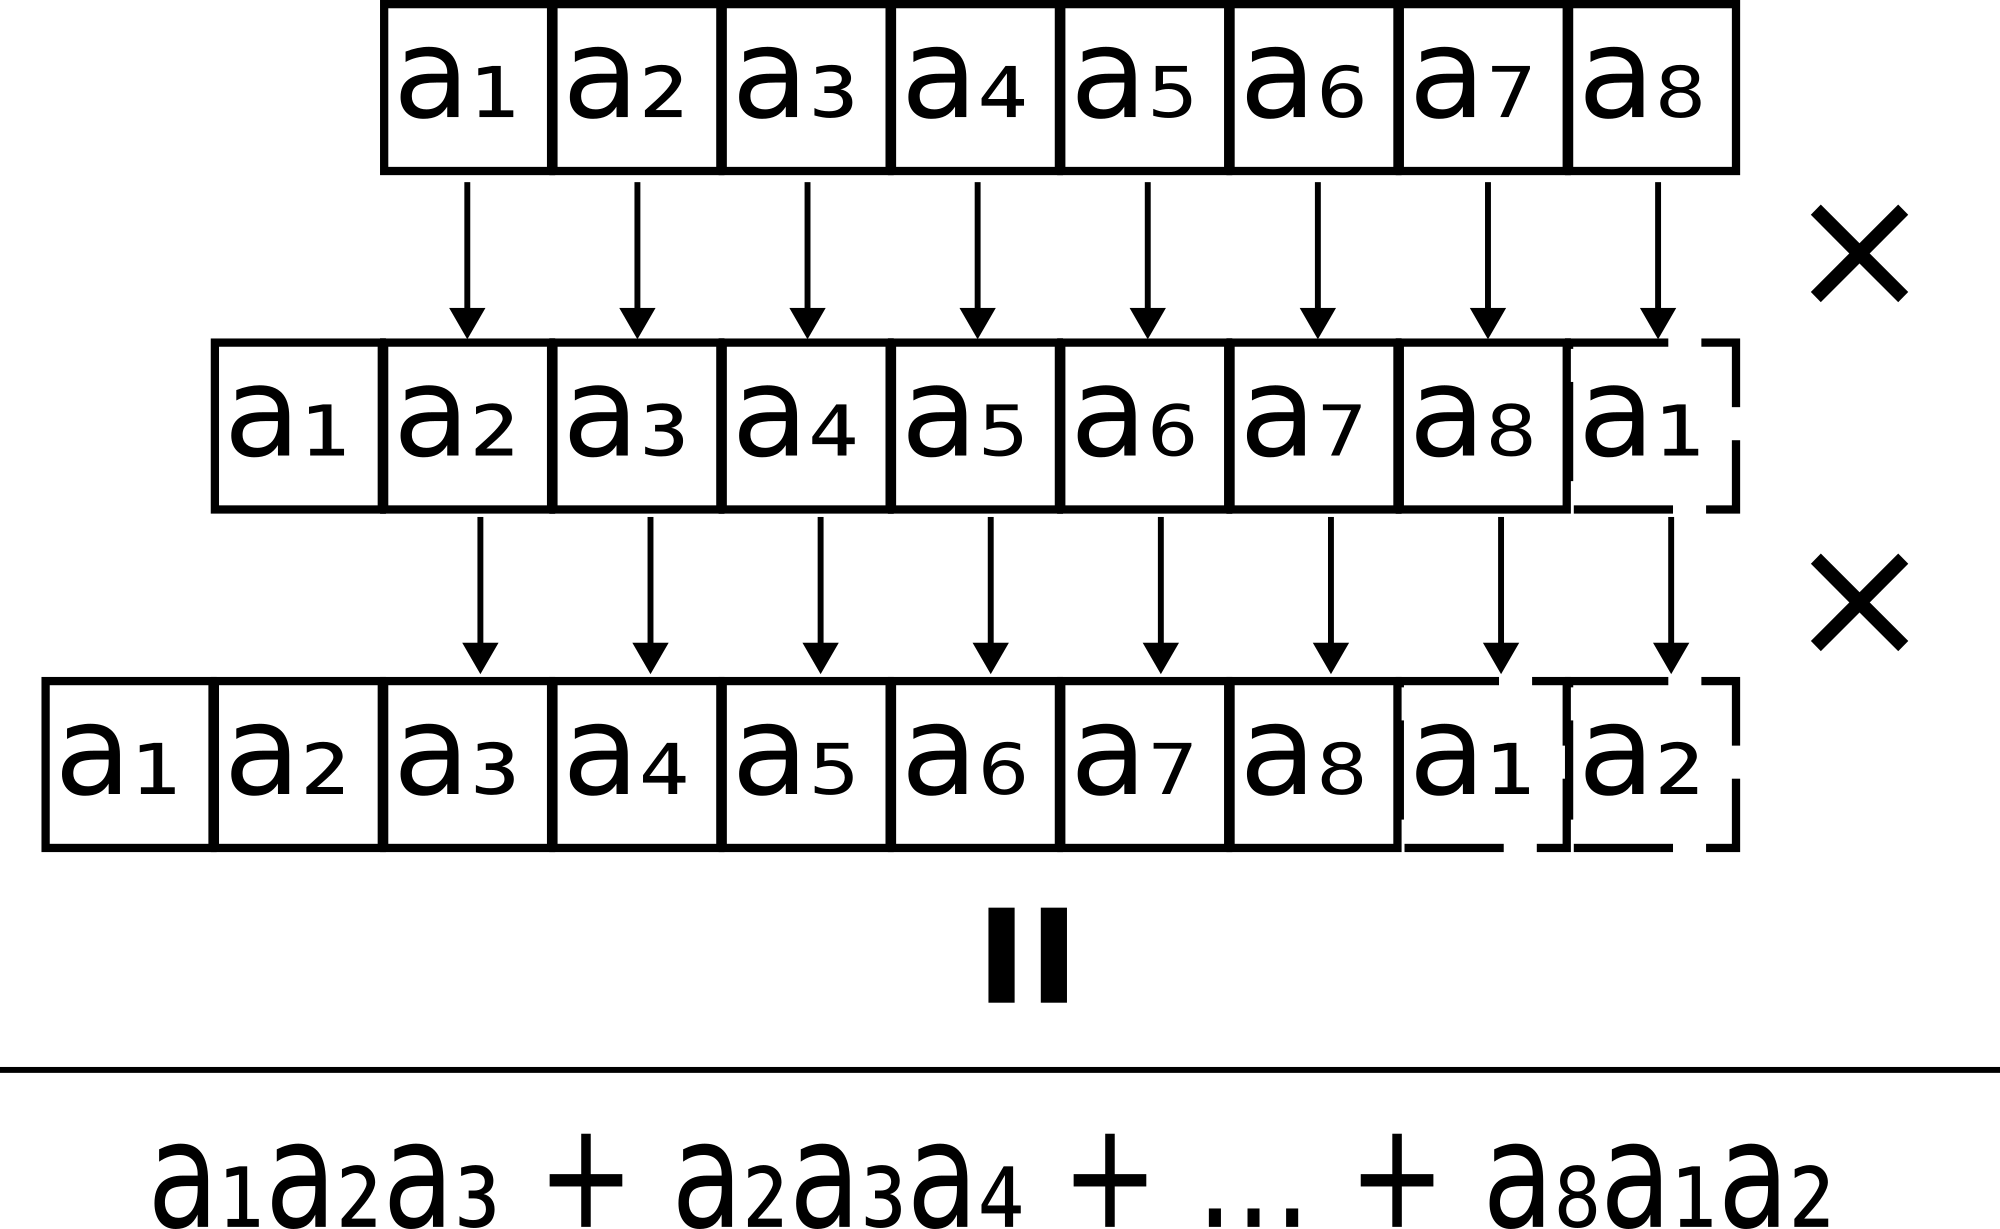
\includegraphics[width=0.45\linewidth]{images/periodic.png}
    \label{fig:s3-periodic}}
  \hfill
  \subfigure[Zero padding]{
    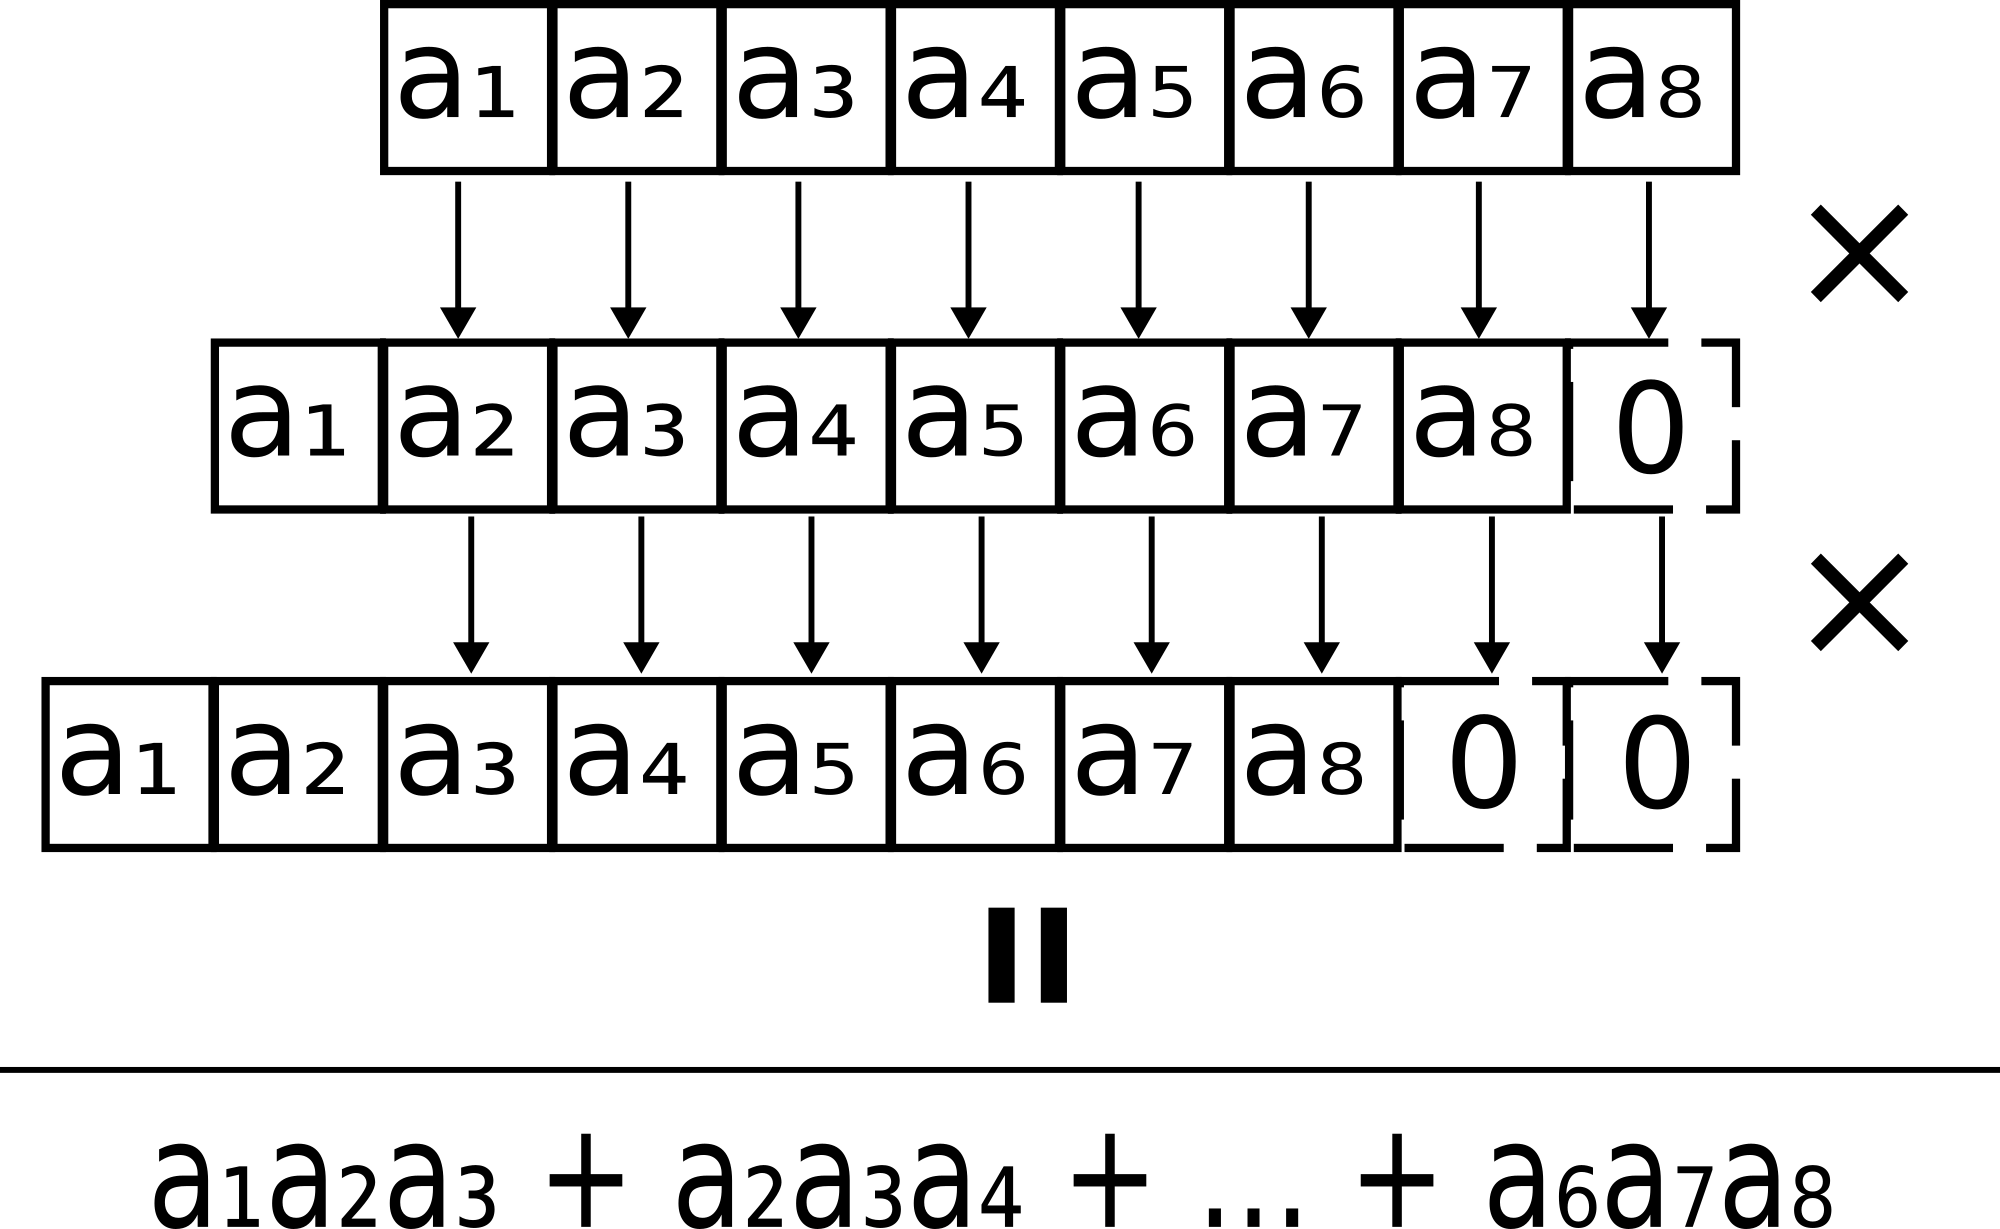
\includegraphics[width=0.45\linewidth]{images/zeros.png}
    \label{fig:s3-zeros}}
  \caption[]{Computation of unnormalized $S_3$ function at point $(1, 2)$ for
    one-dimensional sequence of length 8.}
  \label{fig:s3-computation}
\end{figure*}

The second approach is to compute the whole correlation map in Fourier
domain. Suppose we have a function
$f: \mathbb{R} \rightarrow \mathbb{R}$. Triple correlation for this function is
a function
\begin{equation}
  g(t_1, t_2) = \int f(\tau) f(\tau + t_1) f(\tau + t_2) d \tau
\end{equation}
We can use a well-known formula to compute Fourier image of $g$:
\begin{equation}
  \hat{g}(z_1, z_2) = \hat{f}(z_1) \hat{f}(z_2) \overline{\hat{f}(z_1 + z_2)}
\end{equation}
This algorithm has a better computational complexity compared with the previous
algorithms if the whole correlation map is needed ($O(n^2 \log n)$ vs
$O(n^3)$ where $n$ is a number of elements in the input array). The whole
correlation map, however, requires a lot of memory and is rarely
needed. Imagine, that the input array $A$ is of dimensions $500 \times 500$.
Then, considering that single precision floating point numbers are used,
$4 \cdot 2 \cdot 500^4 / 1000^3 = 500$ GB are needed to store Fourier image of
the map. Moreover, Fourier image of the whole map is needed even if only one
element of the map in spatial domain is required. The aforementioned limitations
render this approach very impractical.

Our implementation fixes $x_1$ and $x_2$ to be parallel to one of the axes $X$,
$Y$ or $Z$ with restriction $x_1 \perp x_2$ (\cref{fig:pattern}). Thus, the
output has dimensions $D_1 \times D_2$ where $D_1$ and $D_2$ are dimensions of
the input array along selected axes.
\begin{figure}[ht]
  \centering
  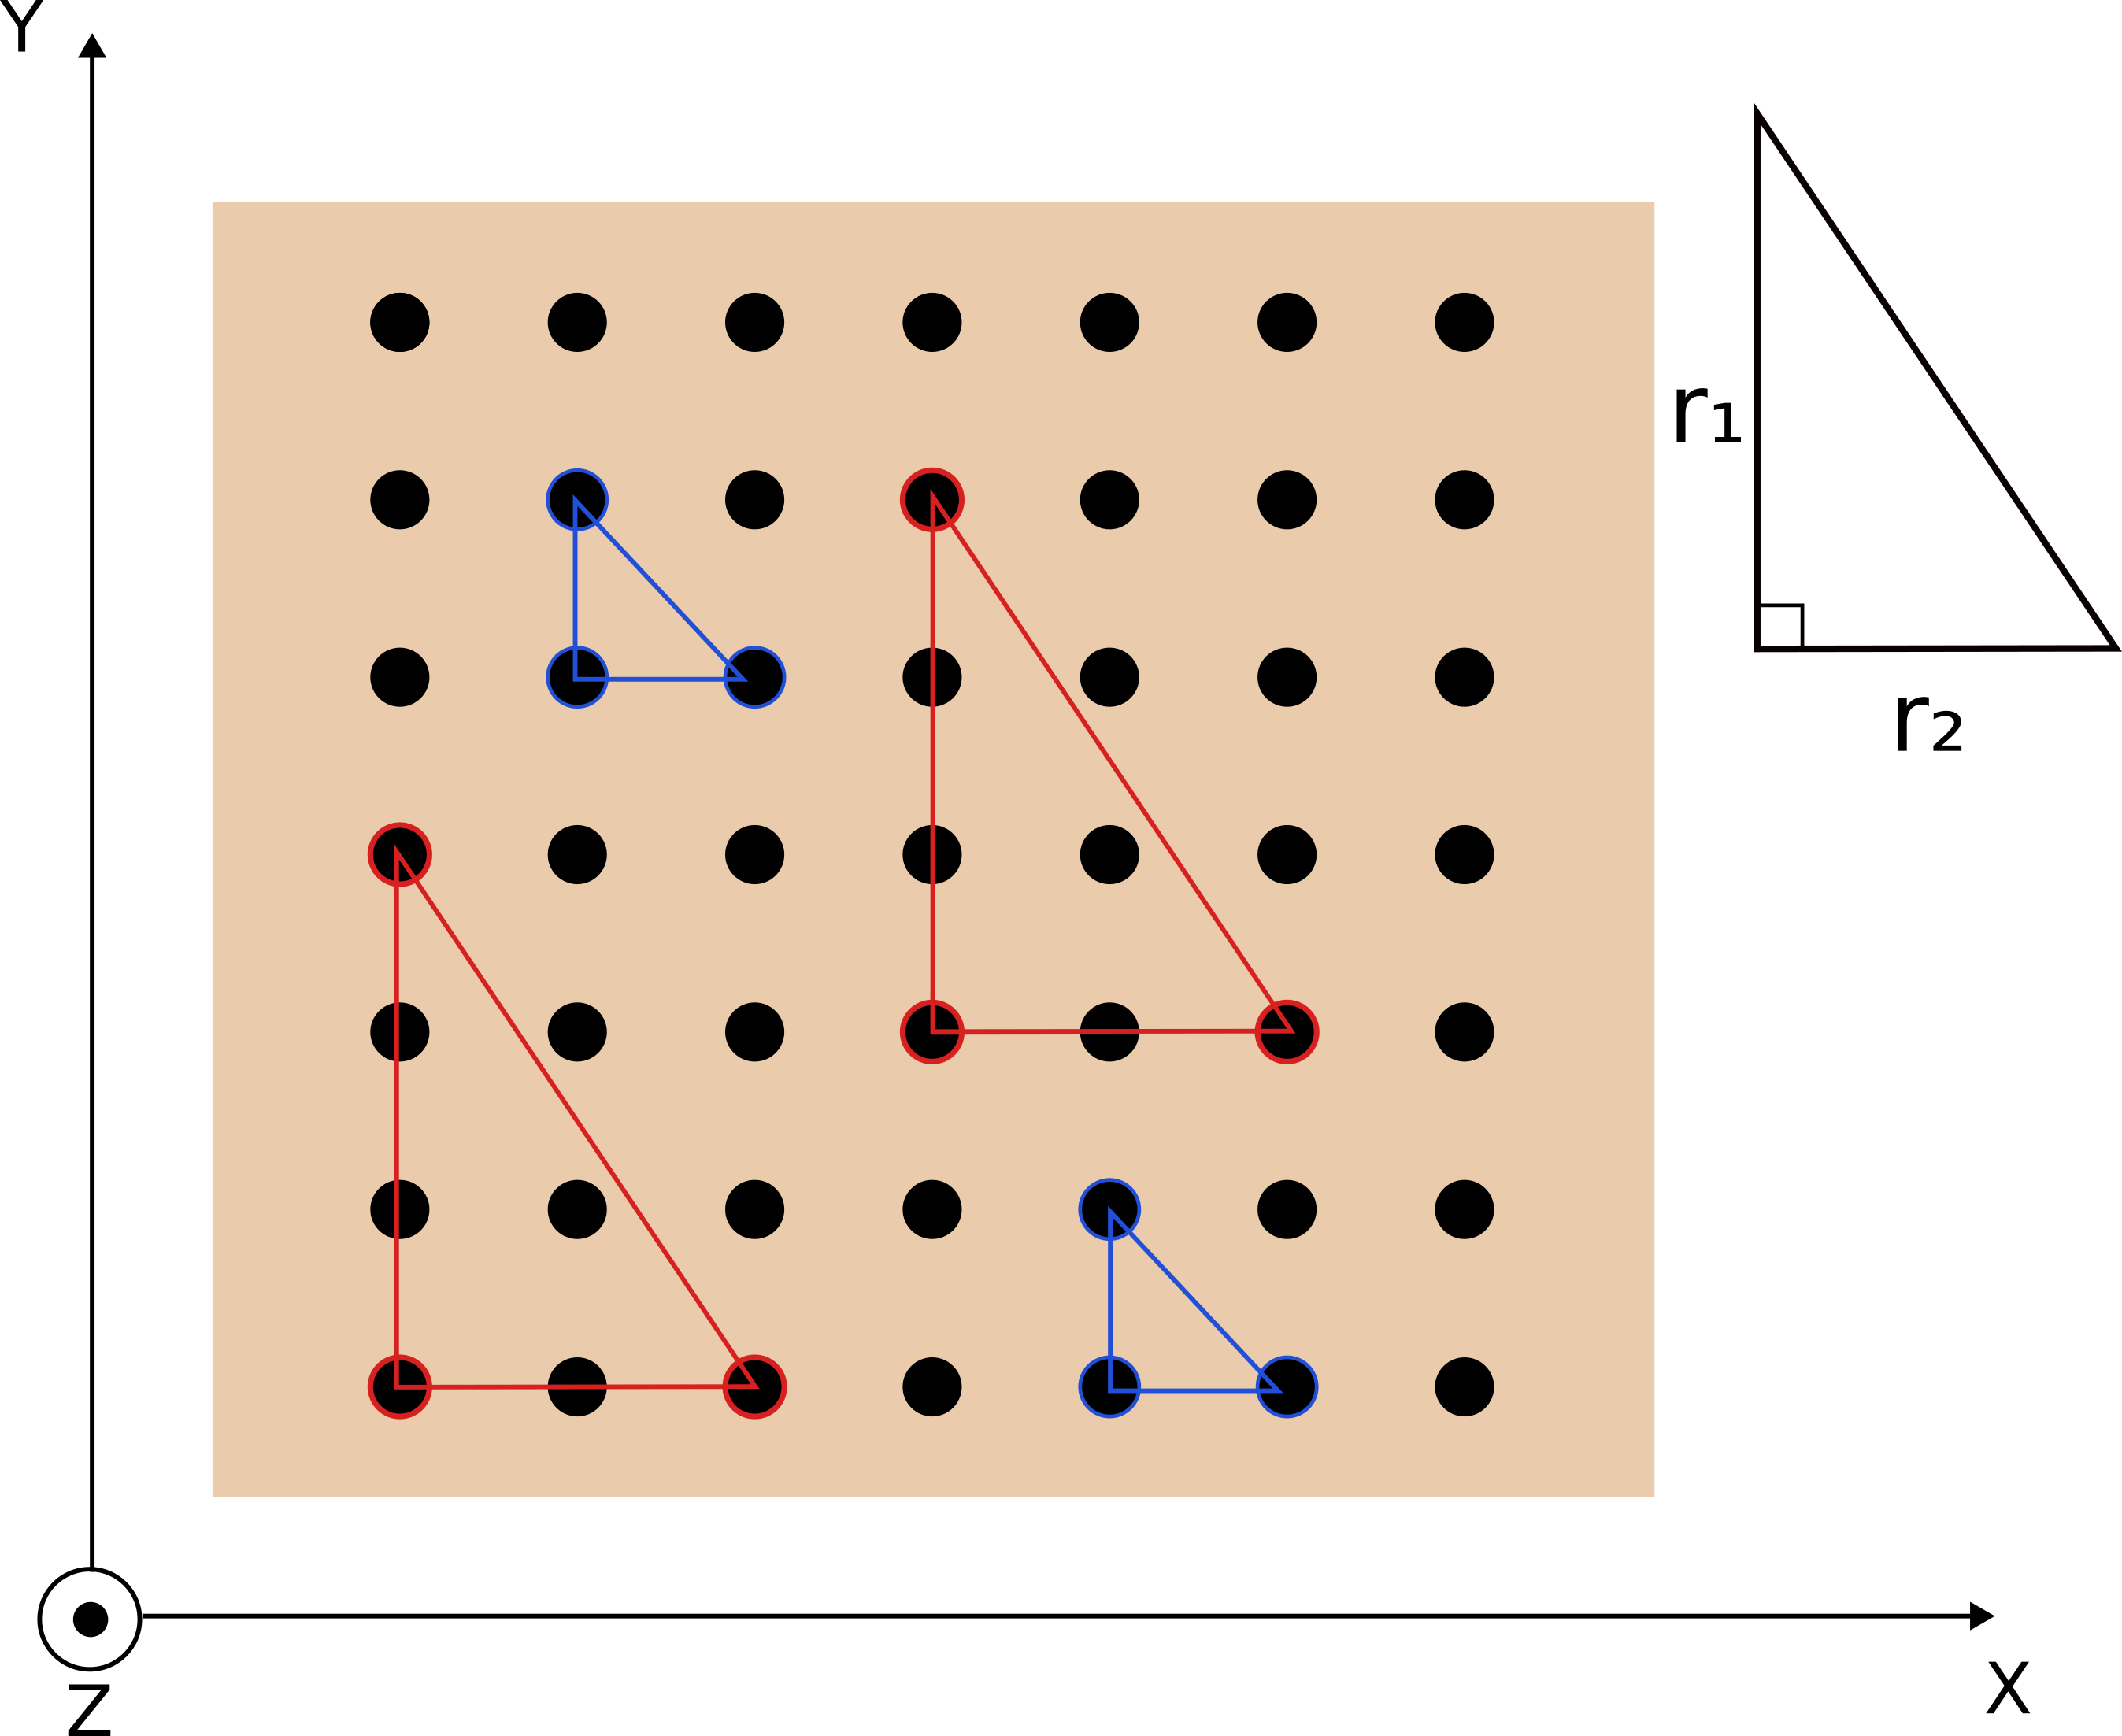
\includegraphics[width=0.5\linewidth]{images/pattern.png}
  \caption[]{The pattern used for calculation of $S_3$ function in our
    implementation. Vectors $x_1$ and $x_2$ are parallel to one of the axes $X$,
    $Y$ or $Z$ and have lengths $r_1$ and $r_2$ respectively. A red triangle
    contributes to $S_3(2, 6)$ and blue triangles contribute to $S_3(1, 1)$.}
  \label{fig:pattern}
\end{figure}

Algorithms for three-point surface functions are the same as for $S_3$,
containing only small modifications. The main difference is that we need to
replace an indicator function $I_n$ with an edge detection operator $E_n$
(see \ref{sec:filter}). Then the algorithms are straightforward:
\begin{algorithmic}[1]
  \Procedure{$F_{sss}$}{$A, n, x_1, x_2$}
  \State $A_n \gets E_n (A)$
  \State $A'_n \gets \mathfrak{S}(A_n, x_1)$
  \State $A''_n \gets \mathfrak{S}(A_n, x_2)$
  \State $T \gets A_n \cdot A'_n \cdot A''_n$
  \State \textbf{return} $Sum(T) / Norm(A, x_1, x_2)$
  \EndProcedure

  \Procedure{$F_{ssv}$}{$A, n, x_1, x_2$}
  \State $A_n \gets E_n (A)$
  \State $A_{(void)} \gets I_{(void)} (A)$
  \State $A'_n \gets \mathfrak{S}(A_n, x_1)$
  \State $A'_{(void)} \gets \mathfrak{S}(A_{(void)}, x_2)$
  \State $T \gets A_n \cdot A'_n \cdot A'_{(void)}$
  \State \textbf{return} $Sum(T) / Norm(A, x_1, x_2)$
  \EndProcedure

  \Procedure{$F_{svv}$}{$A, n, x_1, x_2$}
  \State $A_n \gets E_n (A)$
  \State $A_{(void)} \gets I_{(void)} (A)$
  \State $A'_{(void)} \gets \mathfrak{S}(A_{(void)}, x_1)$
  \State $A''_{(void)} \gets \mathfrak{S}(A_{(void)}, x_2)$
  \State $T \gets A_n \cdot A'_{(void)} \cdot A''_{(void)}$
  \State \textbf{return} $Sum(T) / Norm(A, x_1, x_2)$
  \EndProcedure
\end{algorithmic}

Input images must have appropriately high resolution for edge detection filter
to work correctly. A criterion for ``goodness'' of an image can be expressed
with $C_{\alpha}$ parameter \cite{samarin2023robust}. Let $\alpha \in [0, 1]$
and $f(x)$ be (band-limited) input image ($x \in \mathbb{R}^2$ or
$\mathbb{R}^3$). We define $C_\alpha$ as follows:
\begin{equation}
  \begin{aligned}
    f_0(x) &= f(x) - \langle f(x) \rangle \\
    C_\alpha &= \frac{\int_{-\alpha\omega}^{\alpha\omega} |\hat{f_0}(z)|^2
      dz}{\int_{-\omega}^{\omega} |\hat{f_0}(z)|^2 dz}
  \end{aligned}
\end{equation}
where $\hat{f_0}$ is a Fourier transform of $f_0$ and $\omega$ is a folding
frequency which depends only on resolution of the image. If a criterion
$C_{0.5} > 0.97$ holds then the image is suitable for application of
aforementioned algorithms for calculation of surface functions.

To compute $C_3$ function we need to use a connected-component labeling
algorithm \cite{4728561,PhysRevB.14.3438} to label clusters. Then, again, a
slightly modified algorithm for $S_3$ is used.
\begin{algorithmic}[1]
  \Procedure{$C_3$}{$A, n, x_1, x_2$}
  \State $A_n \gets I_n (A)$
  \State $C_n \gets \mathfrak{C}(A_n)$
  \State $C'_n \gets \mathfrak{S}(C_n, x_1)$
  \State $C''_n \gets \mathfrak{S}(C_n, x_2)$
  \State $T \gets C_n \odot C'_n \odot C''_n$
  \State \textbf{return} $Sum(T) / Norm(A, x_1, x_2)$
  \EndProcedure
\end{algorithmic}
Here $\mathfrak{C}$ is connected-component labeling operator and $\odot$ is
defined as follows:
\begin{equation}
  x \odot y = \left\{
  \begin{array}{ll}
    1 & \quad x = y \\
    0 & \quad \text{otherwise}
  \end{array}
  \right.
\end{equation}

\section{Verification}
To verify correctness of computation of $S_3$ and $C_3$ functions we use the
following simple relations:
\begin{align}
  S_3^n (x, 0) = S_3^n (0, x) &= S_2^n(x) \\
  C_3^n (x, 0) = C_3^n (0, x) &= C_2^n(x) \\
  \lim_{\substack{x_1 \to \infty \\ x_2 \to \infty}} S_3^n (x_1, x_2) &= \phi_n^3
\end{align}
Here $\phi_n$ is a fraction of phase $n$ in $A$.

There are only few sets for which analytic expressions for $S_2$ are known. One
of those is a set consisting of overlapping balls with a fixed radius $R$ and
centers generated with Poisson process with parameter $\lambda$. In this case
the expression for $S_2$ is following:
\begin{equation}
  \begin{aligned}
    S_2(r, R) &= \exp(-\frac{4}{3}\pi\lambda R^3 f(r, R)) \\
    f(r, R) &= \left\{
    \begin{array}{ll}
      1 + \frac{3}{4} \frac{r}{R} - \frac{1}{16} (\frac{r}{R})^3 & \quad r < 2R \\
      2 & \quad \text{otherwise}
    \end{array}
    \right.
  \end{aligned}
  \label{eq:s2-balls}
\end{equation}

On \cref{fig:balls} there is an intersection of such a set with $R = 0.02$ and
$\lambda=5000$ and a cube $[0, 1]^3$. Because $R \ll 1$, we can use
\cref{eq:s2-balls} to verify our computations what we do on
\cref{fig:balls-s3-comparison}.
\begin{figure*}[tp]
  \centering
  \subfigure[Realization of overlapping balls]{
    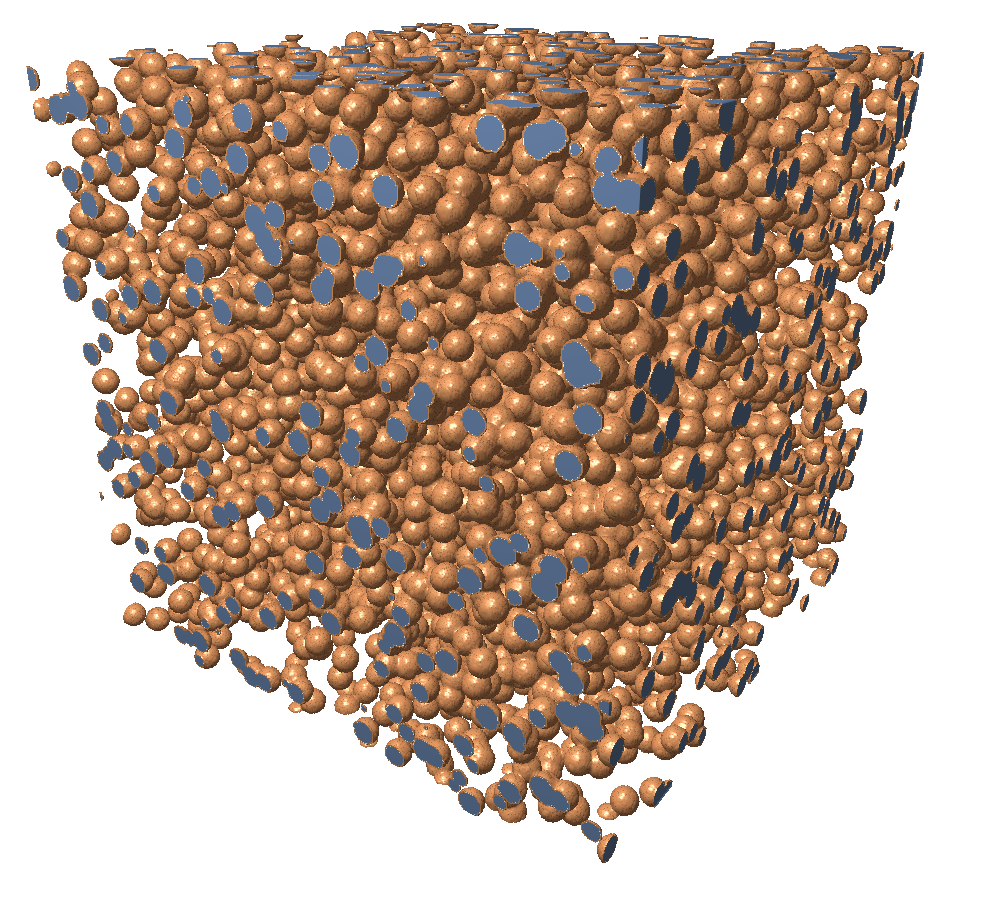
\includegraphics[width=0.45\linewidth]{images/balls.png}
    \label{fig:balls}}
  \hfill
  \subfigure[A plot of $S_3(0, r)$ computed with our algorithm and theoretical
    formula.]{
    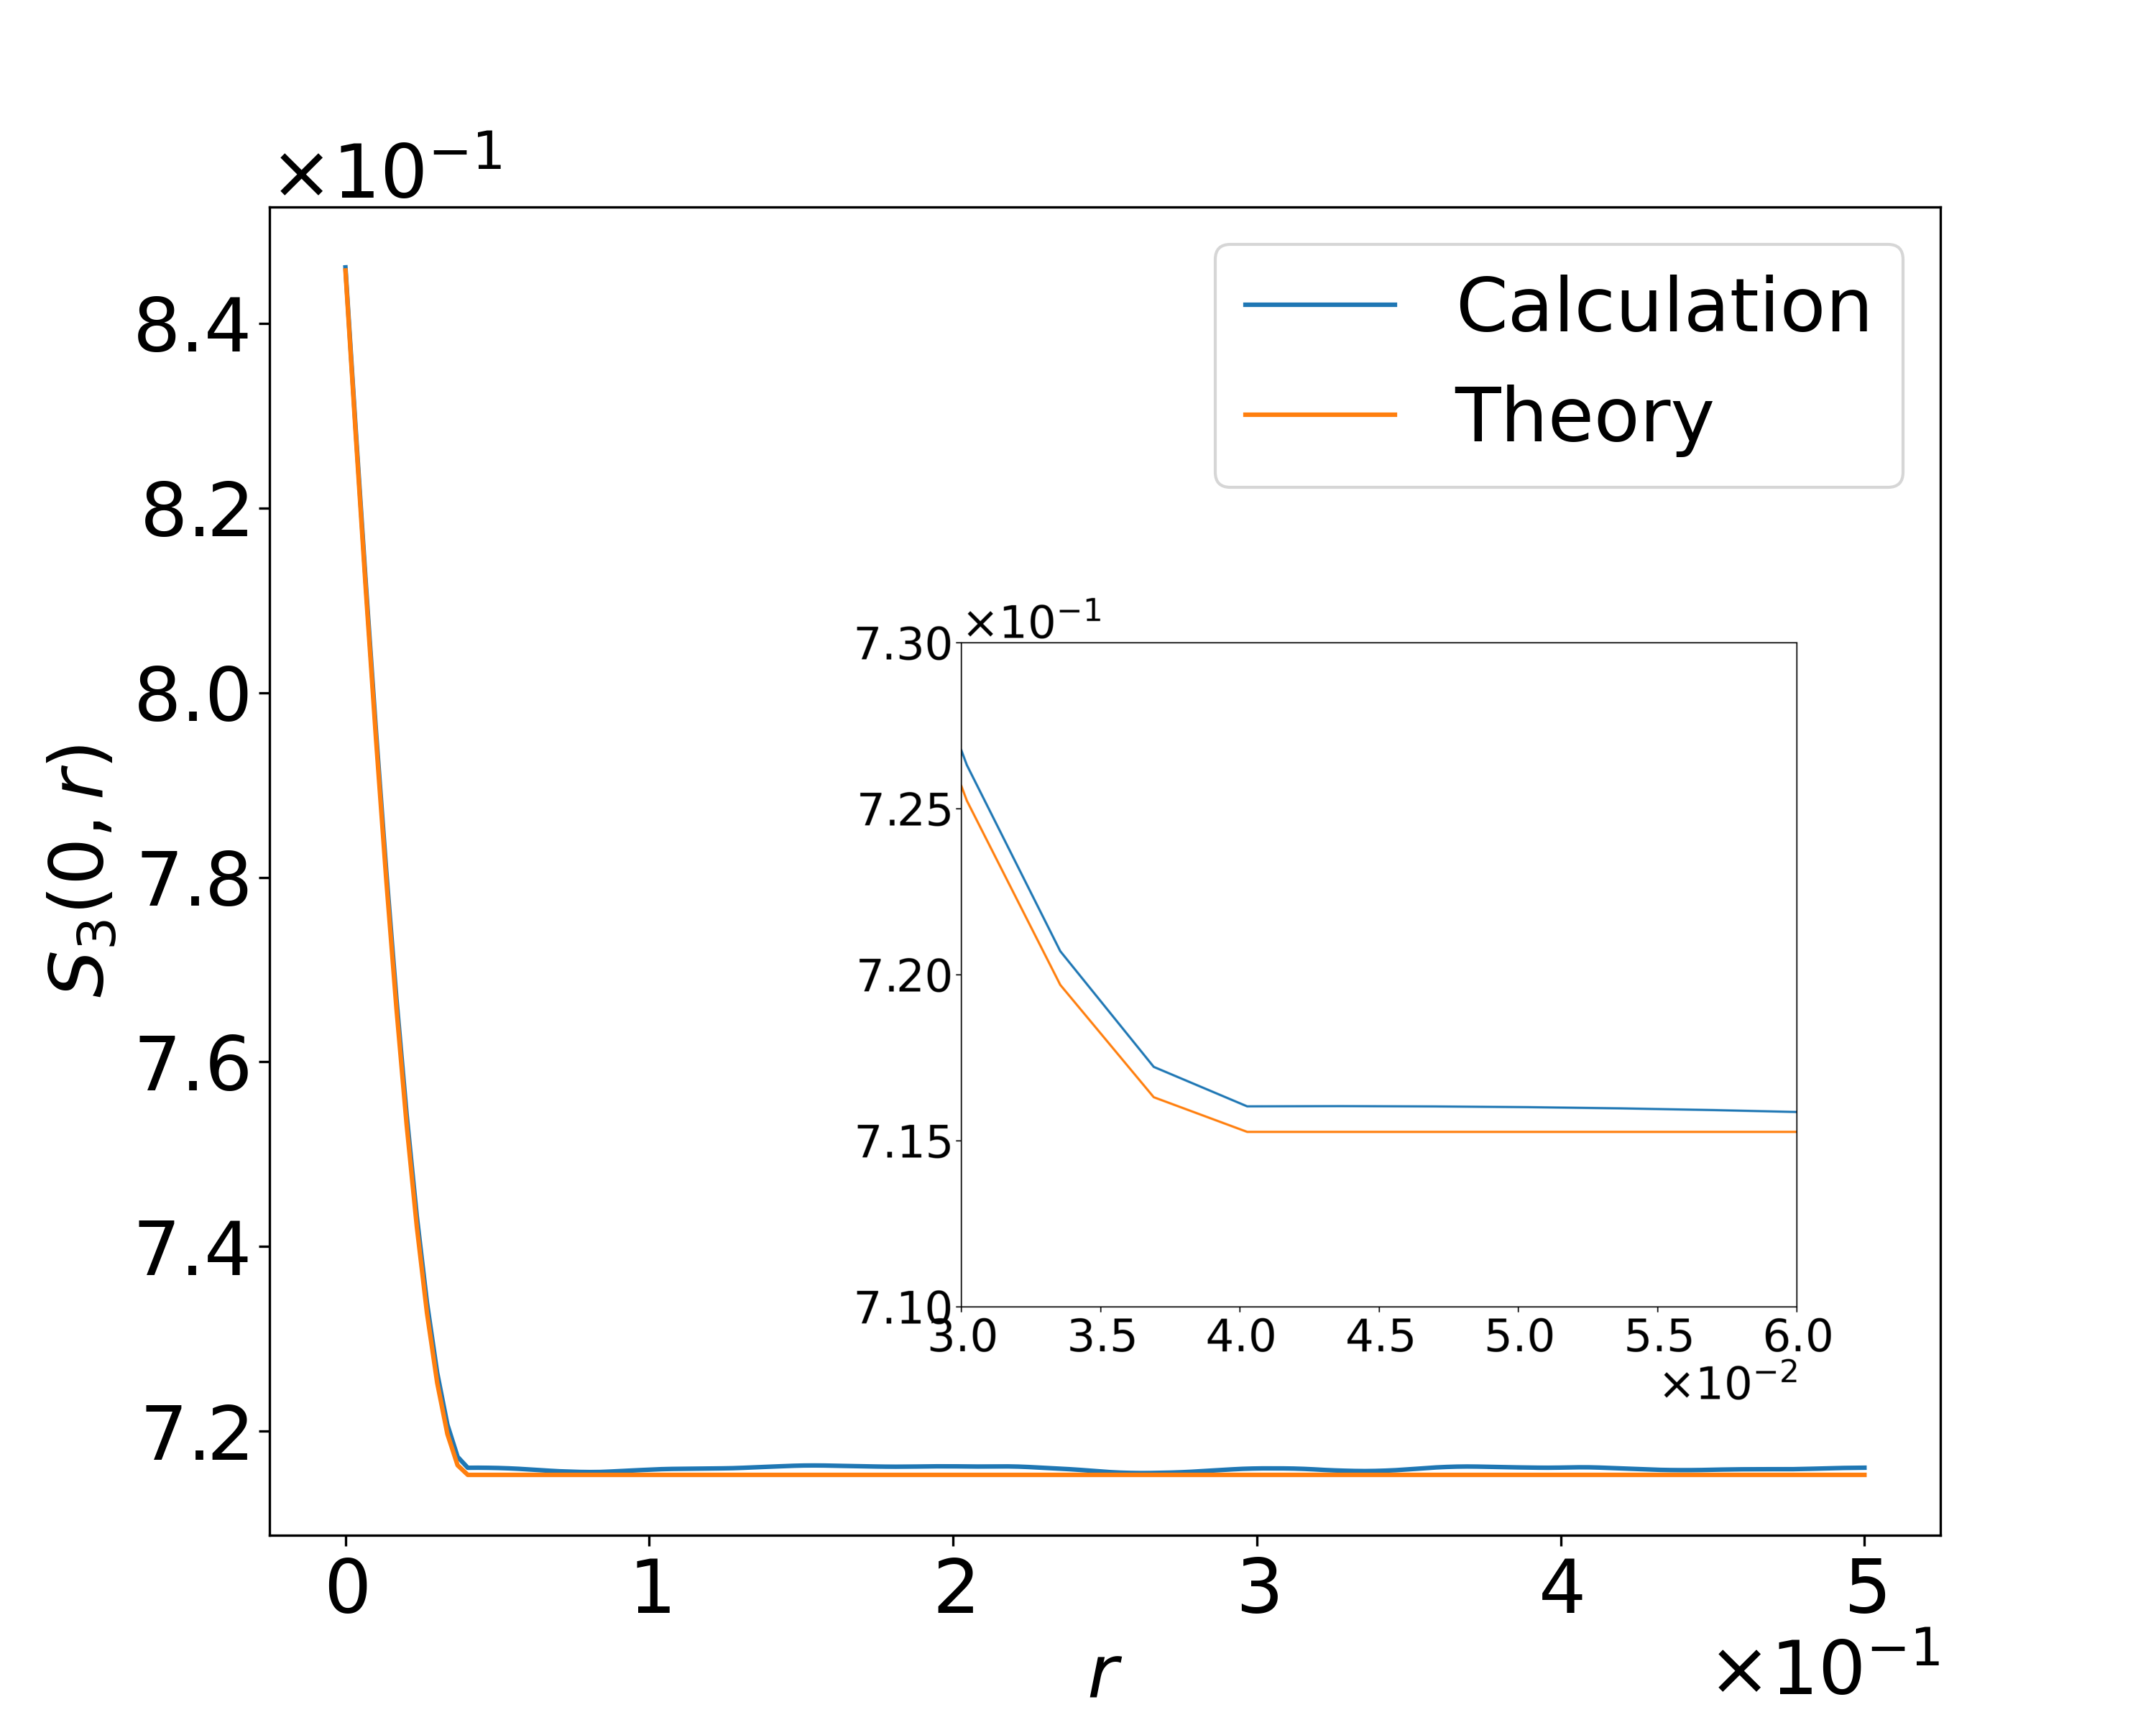
\includegraphics[width=0.45\linewidth]{images/balls-s3.png}
    \label{fig:balls-s3-comparison}}
  \caption[]{A comparison of calculated and theoretical values of $S_3$ function
    for overlapping balls.}
  \label{fig:s3-verification}
\end{figure*}

To test $F_{sss}$ function we use a recently developed approach which computes
that function for sets defined by inequation $f(x) \le T$, $x \in \mathbb{R}^3$
with help of automatic differentiation \cite{postnicov20232}. We choose $f$
\begin{equation}
  f(x, y, z) = (|2x|^{\frac{3}{2}} + |y|^{\frac{3}{2}} + |z|^{\frac{3}{2}})^{\frac{2}{3}}
\end{equation}
so inequation $f(x, y, z) \le T$ gives us an ellipsoid-like object
(\cref{fig:sss-ellipsoid}).

The test was performed by evaluating the inequation with the parameter $T = 0.4$
in a cube $[-1, 1]^3$ and comparing $F_{sss}$ calculated by our algorithm with
precise values. Pointwise relative error of $F_{sss}$ is on
\cref{fig:sss-ellipsoid-error}. Maximal relative error in the area bound by
inequations $x > 0.1$, $y > 0.1$ and $f(x, y) < 0.78$ is about 10\%.
\begin{figure*}[tp]
  \centering
  \subfigure[The ellipsoid-like object used in testing of $F_{sss}$ computation]{
    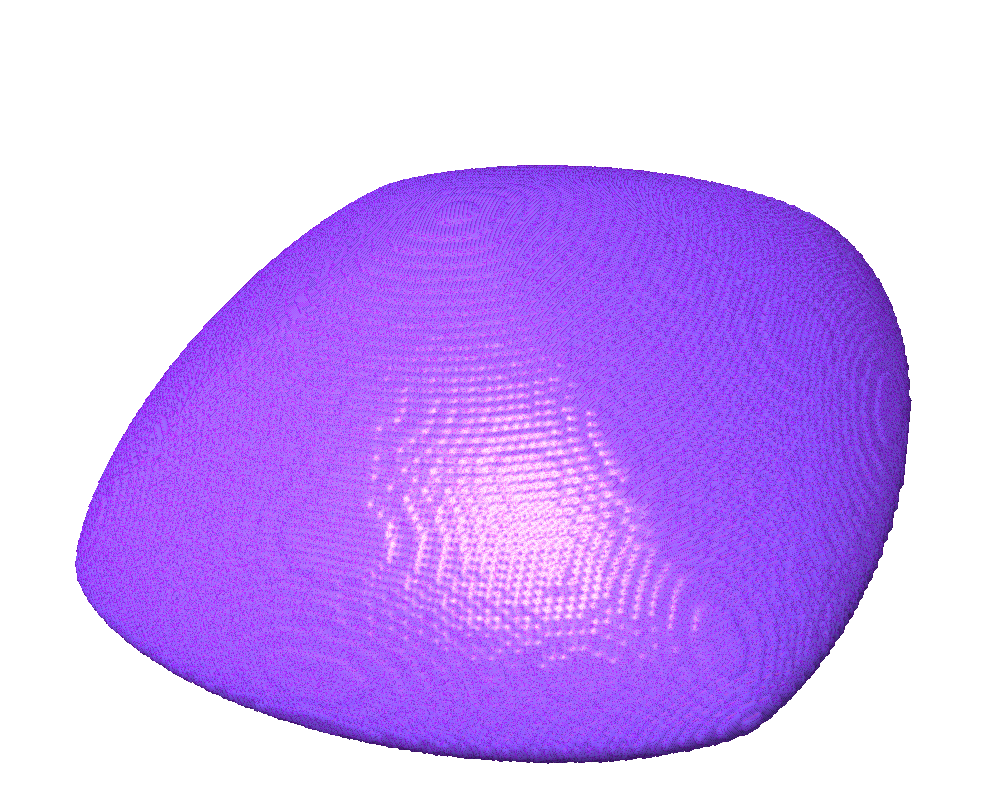
\includegraphics[width=0.45\linewidth]{images/ellipsoid.png}
    \label{fig:sss-ellipsoid}}
  \hfill
  \subfigure[Relative error of computation]{
    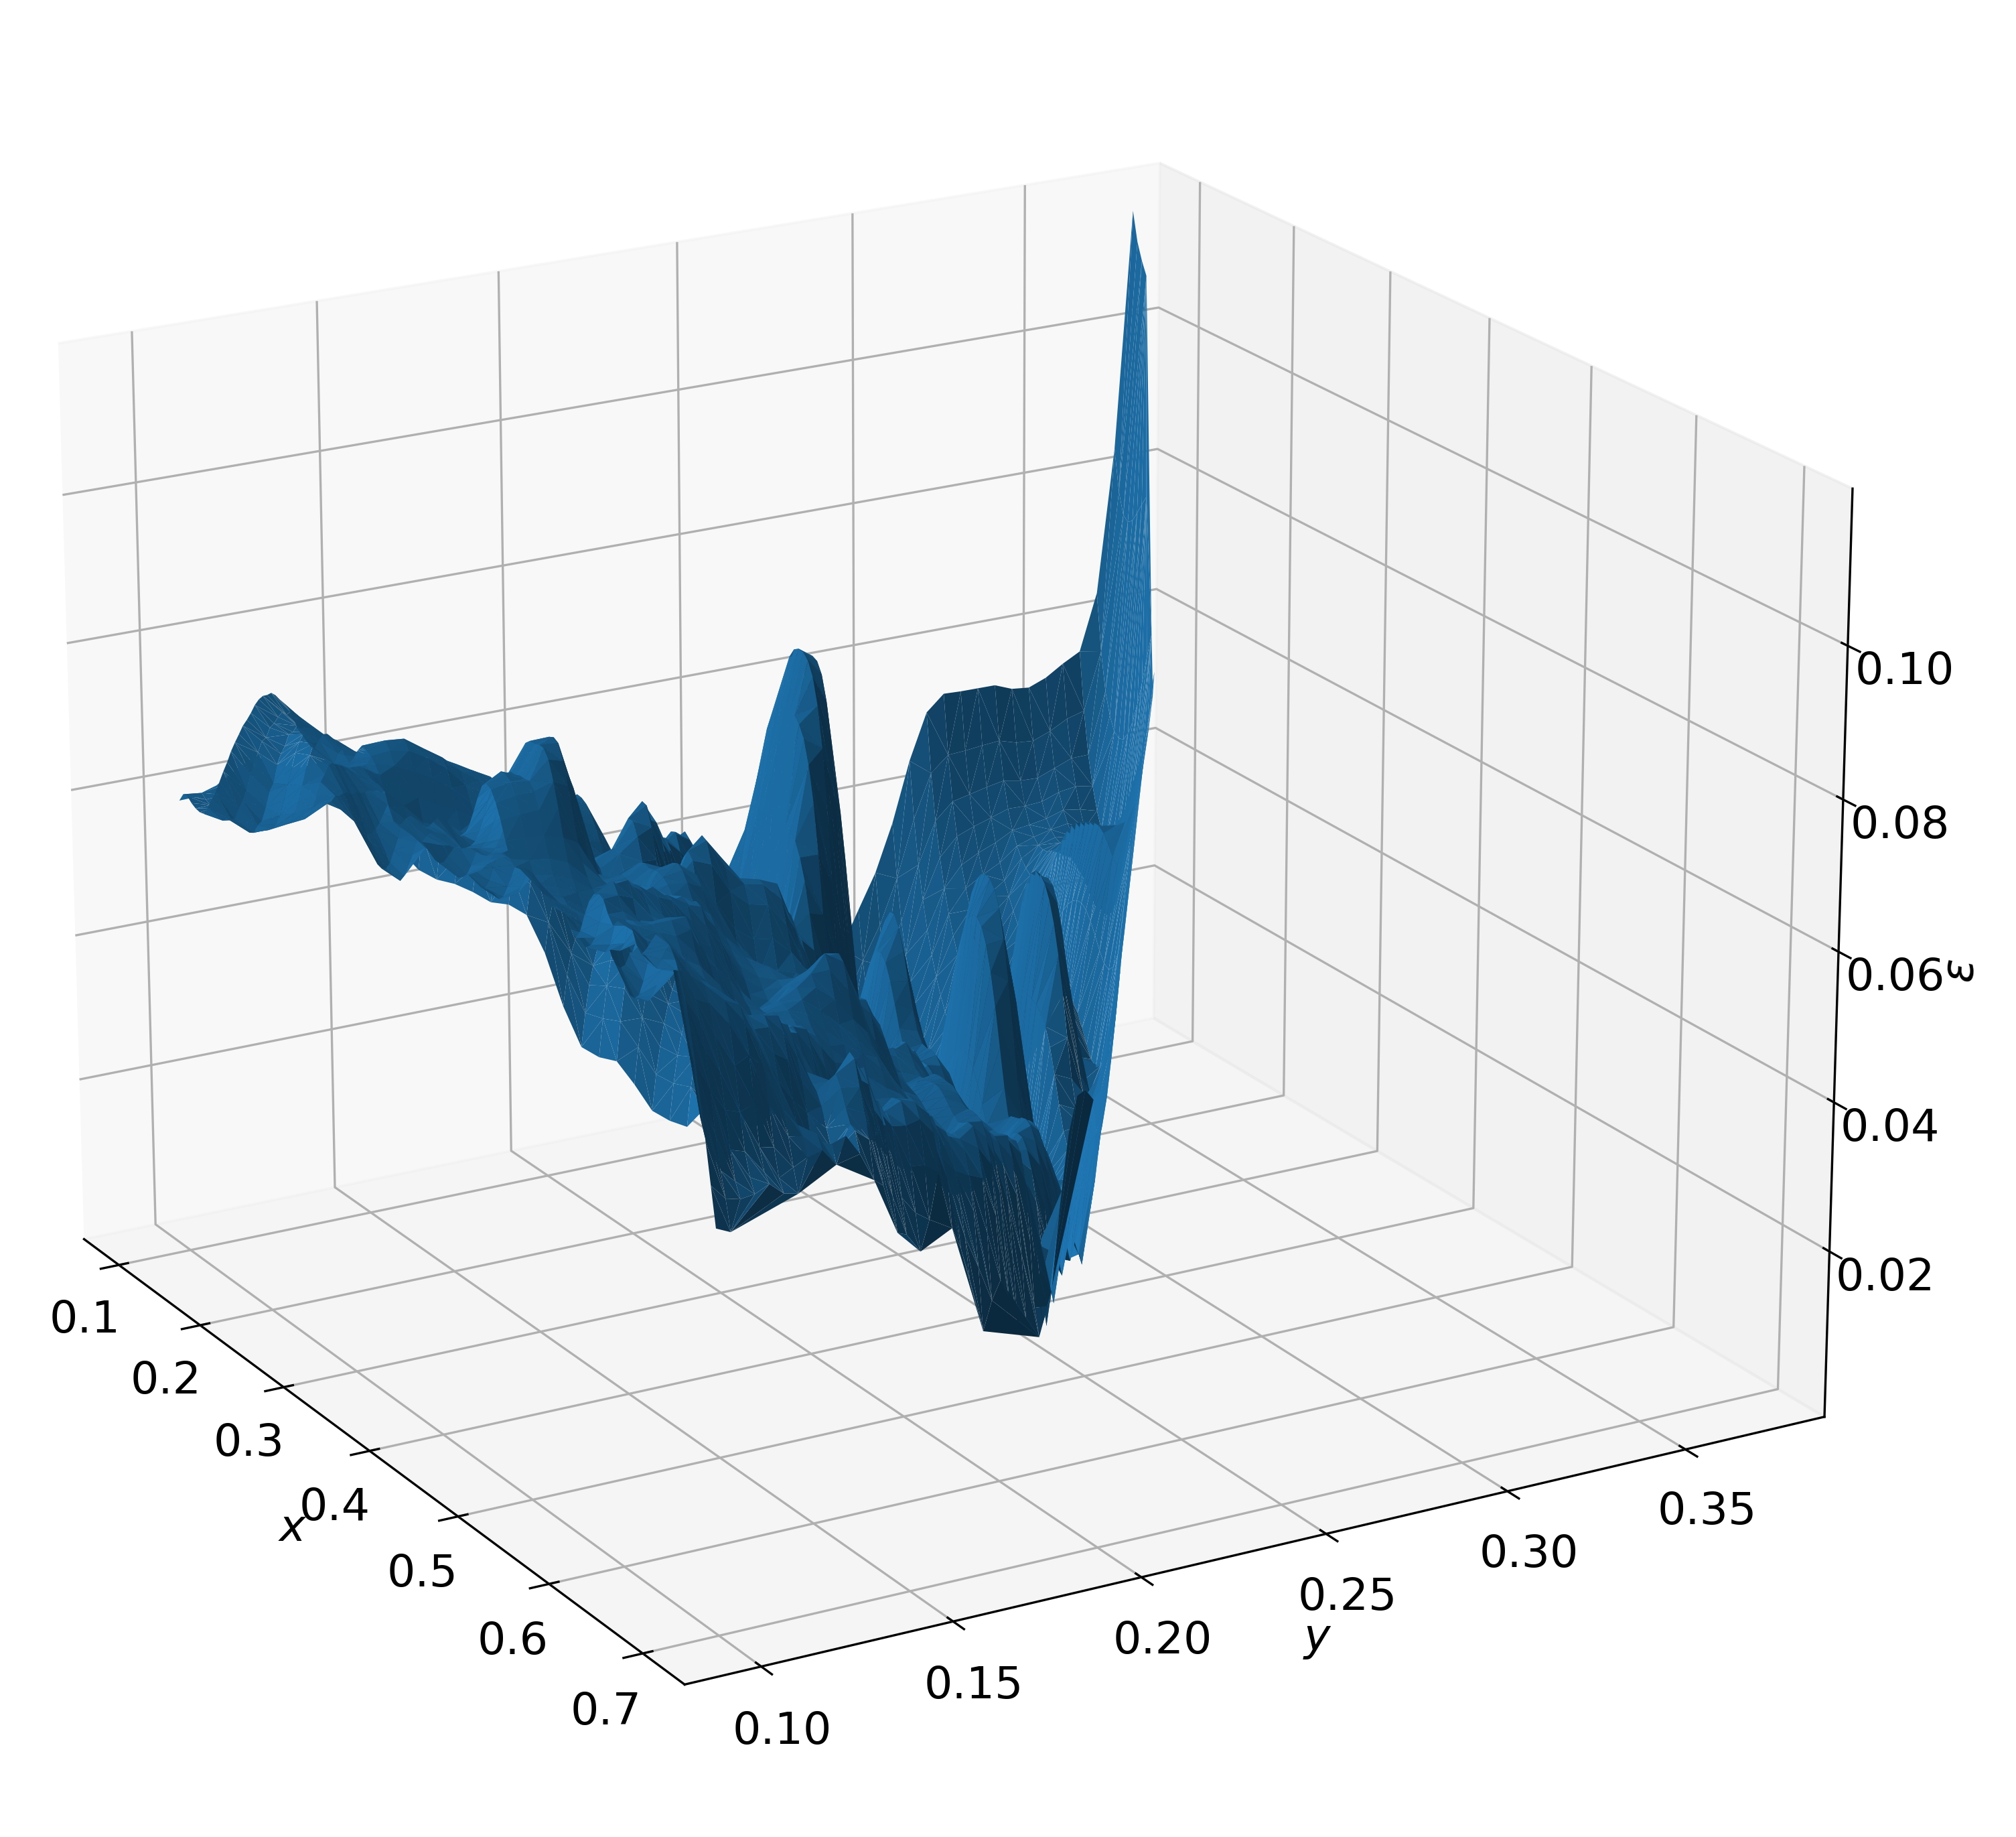
\includegraphics[width=0.45\linewidth]{images/ellipsoid-sss-diff.png}
    \label{fig:sss-ellipsoid-error}}
  \vskip\baselineskip
  \subfigure[$F_{sss}$: precise]{
    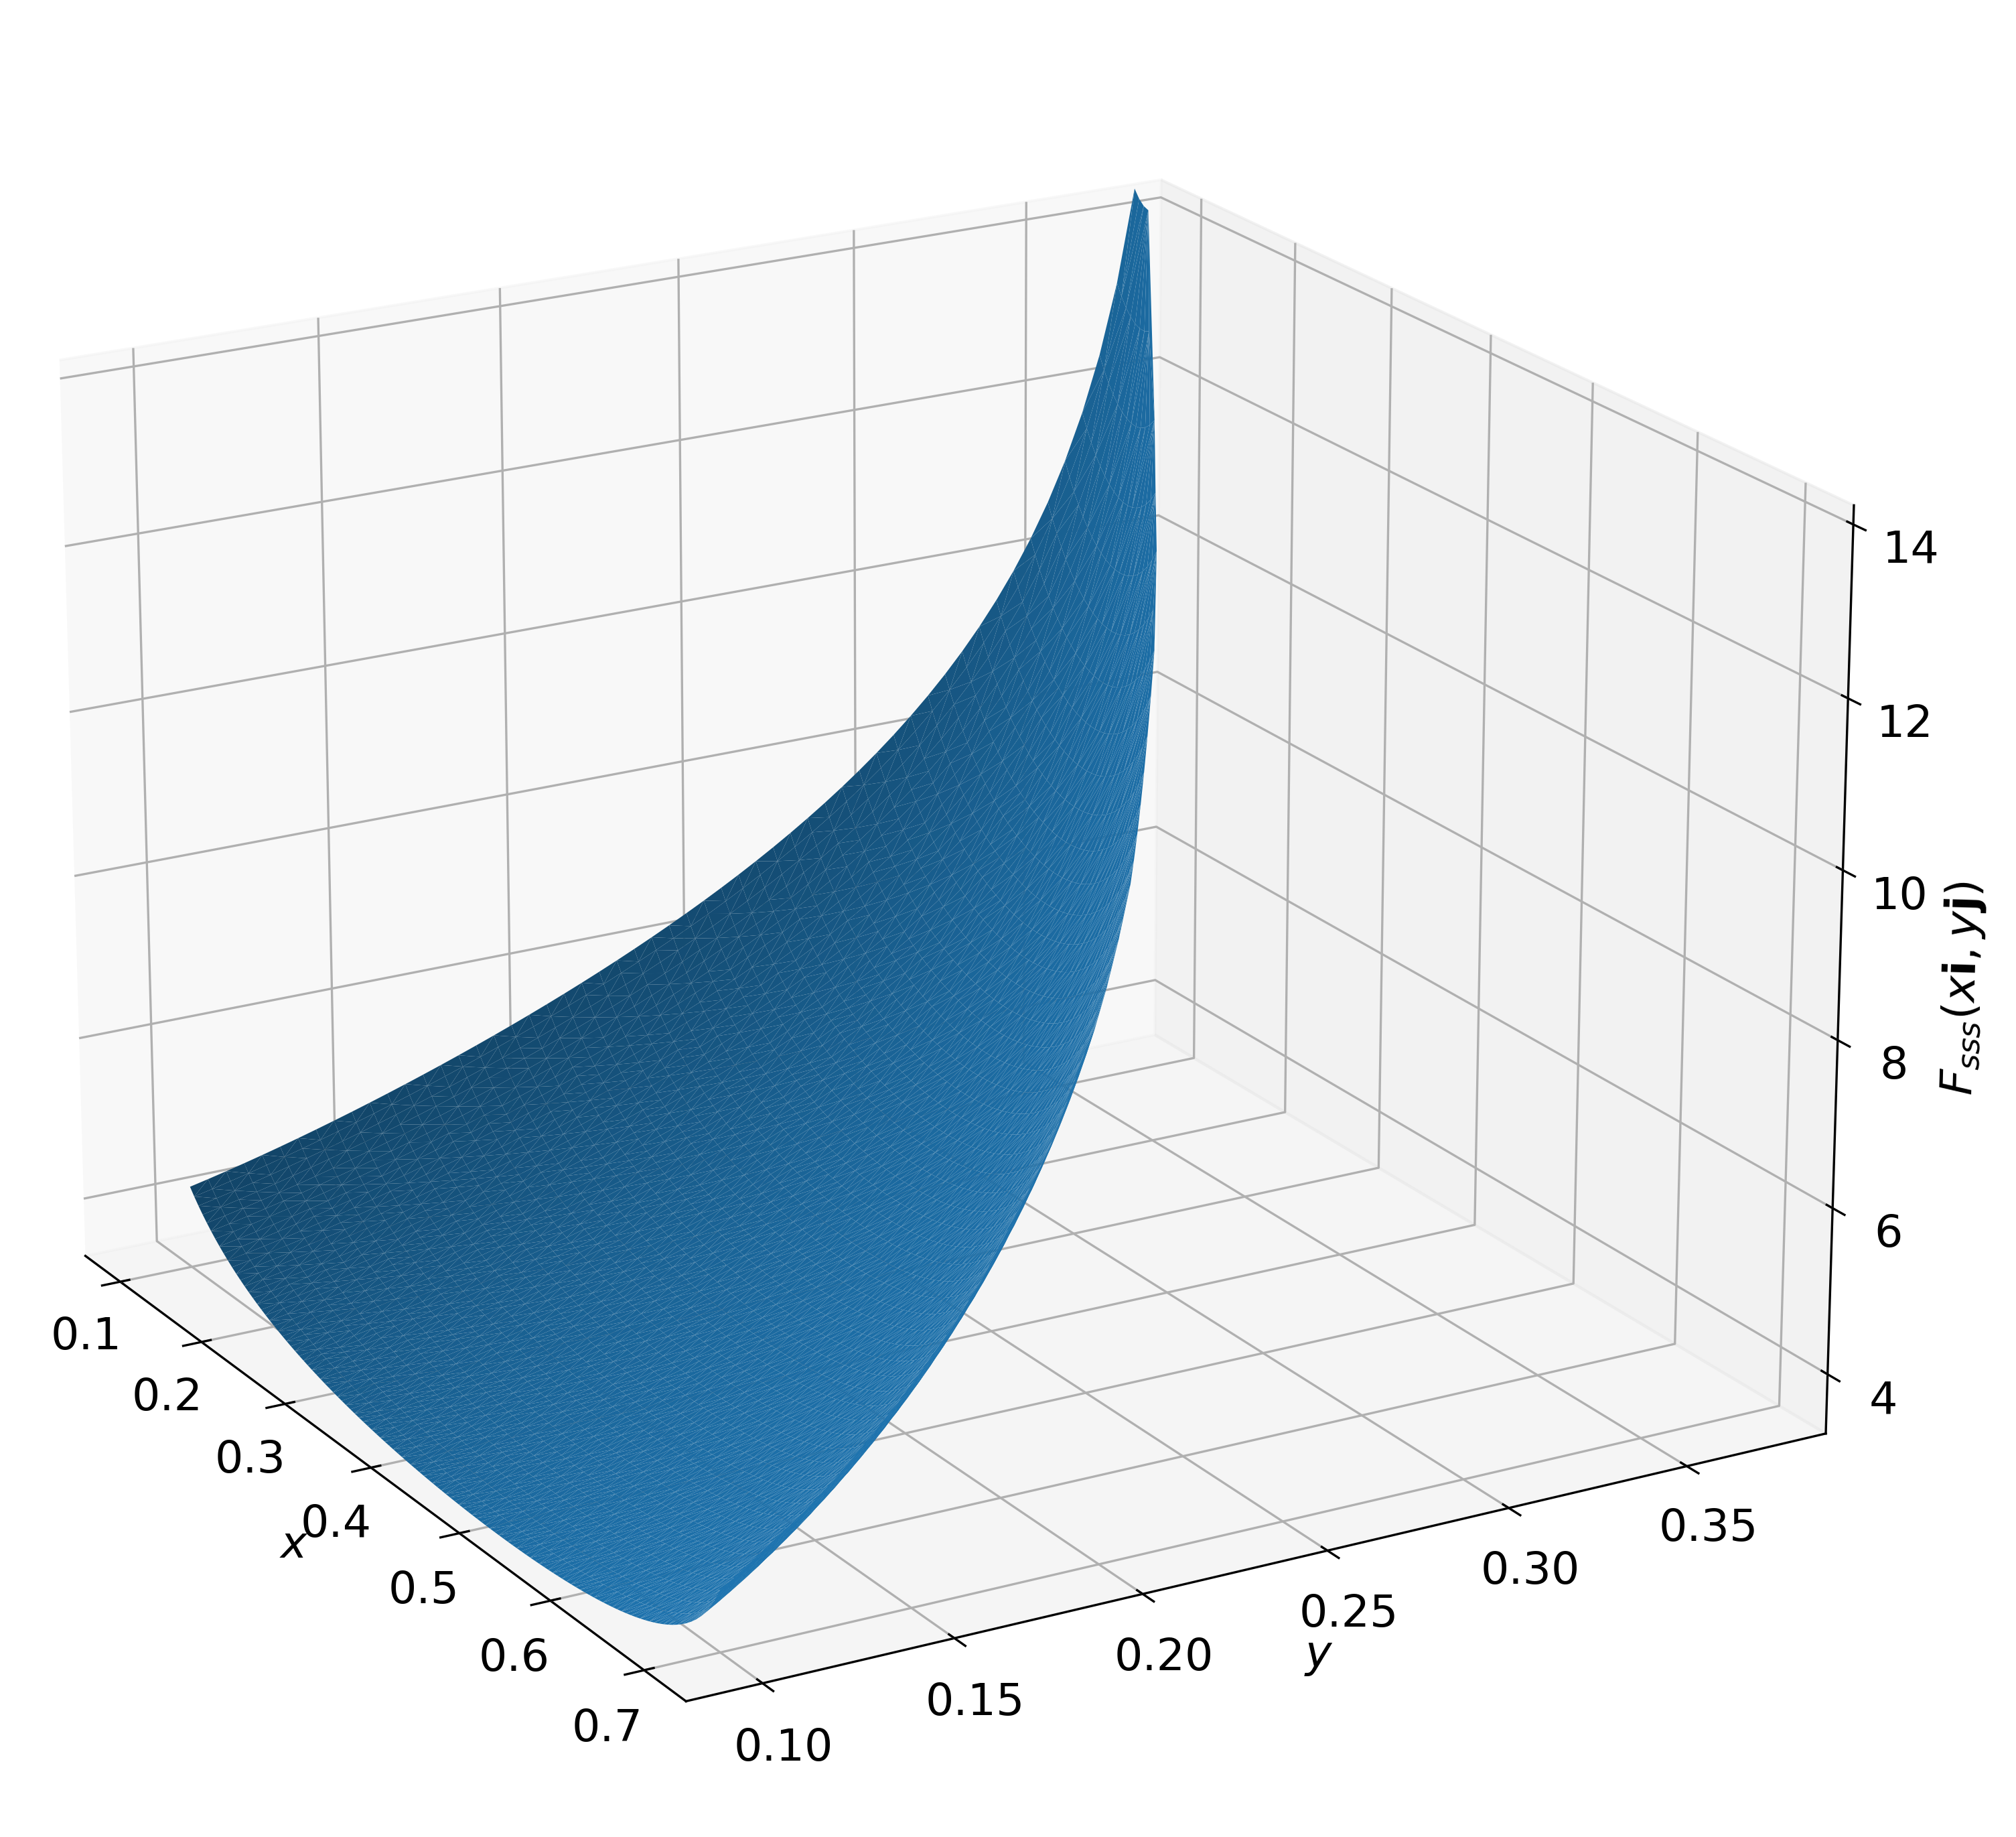
\includegraphics[width=0.45\linewidth]{images/ellipsoid-sss.png}}
  \hfill
  \subfigure[$F_{sss}$: calculated with our approach]{
    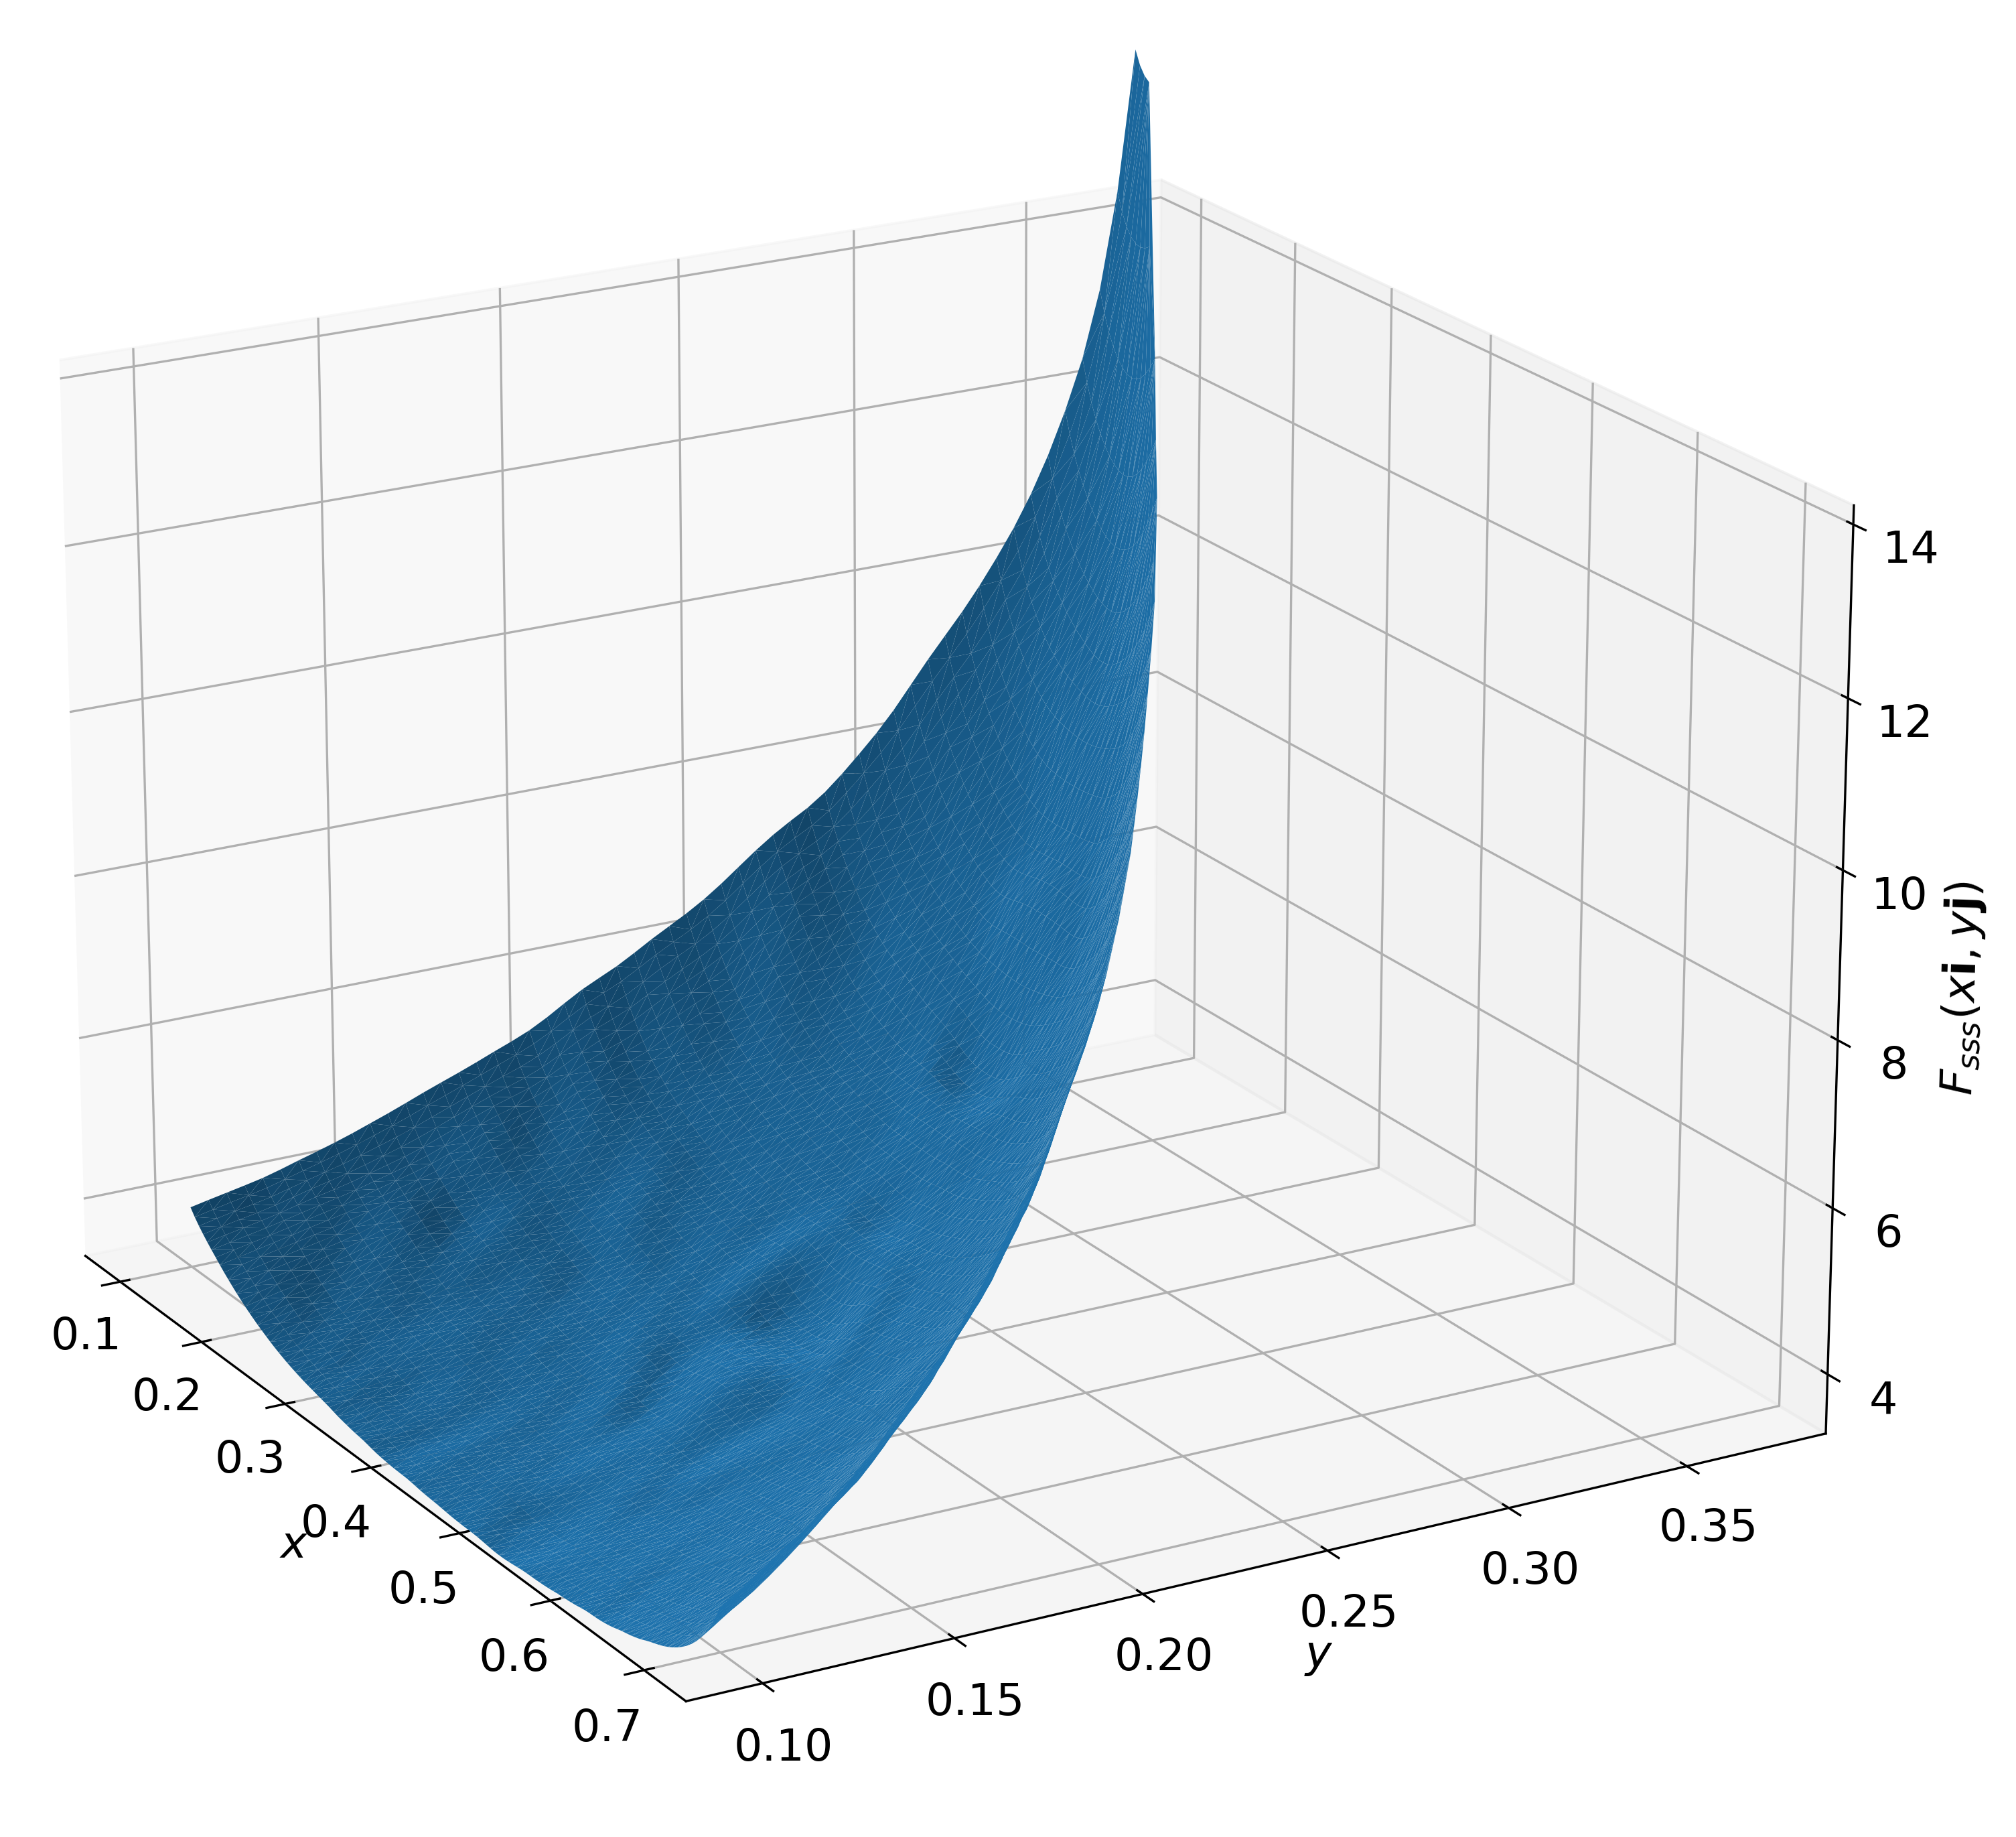
\includegraphics[width=0.45\linewidth]{images/ellipsoid-sss-julia.png}}
  \caption[]{A comparison of $F_{sss}$ function calculated using our approach
    with its precise values.}
  \label{fig:sss-verification}
\end{figure*}

To test $F_{ssv}$ and $F_{svv}$ we use the following relations for such a set
$A$ where all non-void phase is covered by a ball $\mathfrak{O}(R)$:
\begin{align}
  F^n_{ssv}(x_1, x_2) &= F^n_{ss}(x_1) \qquad x_2 > R \\
  F^n_{svv}(x_1, x_2) &= F^n_{sv}(x_1) \qquad x_2 > R
\end{align}
$F_{ss}$ and $F_{sv}$ functions are well-known for a ball of radius $R$ (solid
phase) placed in the center of cube of volume $V$ (void phase):
\begin{align}
  F_{ss}(r, R) &= \frac{1}{V} \left\{
    \begin{array}{ll}
      2\pi R^2/r & \quad r < 2R \\
      0 & \quad \text{otherwise}
    \end{array}
    \right.\\
  F_{sv}(r, R) &= \frac{1}{V} \left\{
    \begin{array}{ll}
      \pi Rr + 2\pi R^2 & \quad r < 2R \\
      4\pi R^2 & \quad \text{otherwise}
    \end{array}
    \right.
\end{align}
The comparison of our algorithm against theory is on
\cref{fig:surface-verification}. Radius of the ball is chosen $R=0.2$.
\begin{figure*}[tp]
  \centering
  \subfigure[$F_{ssv}$]{
    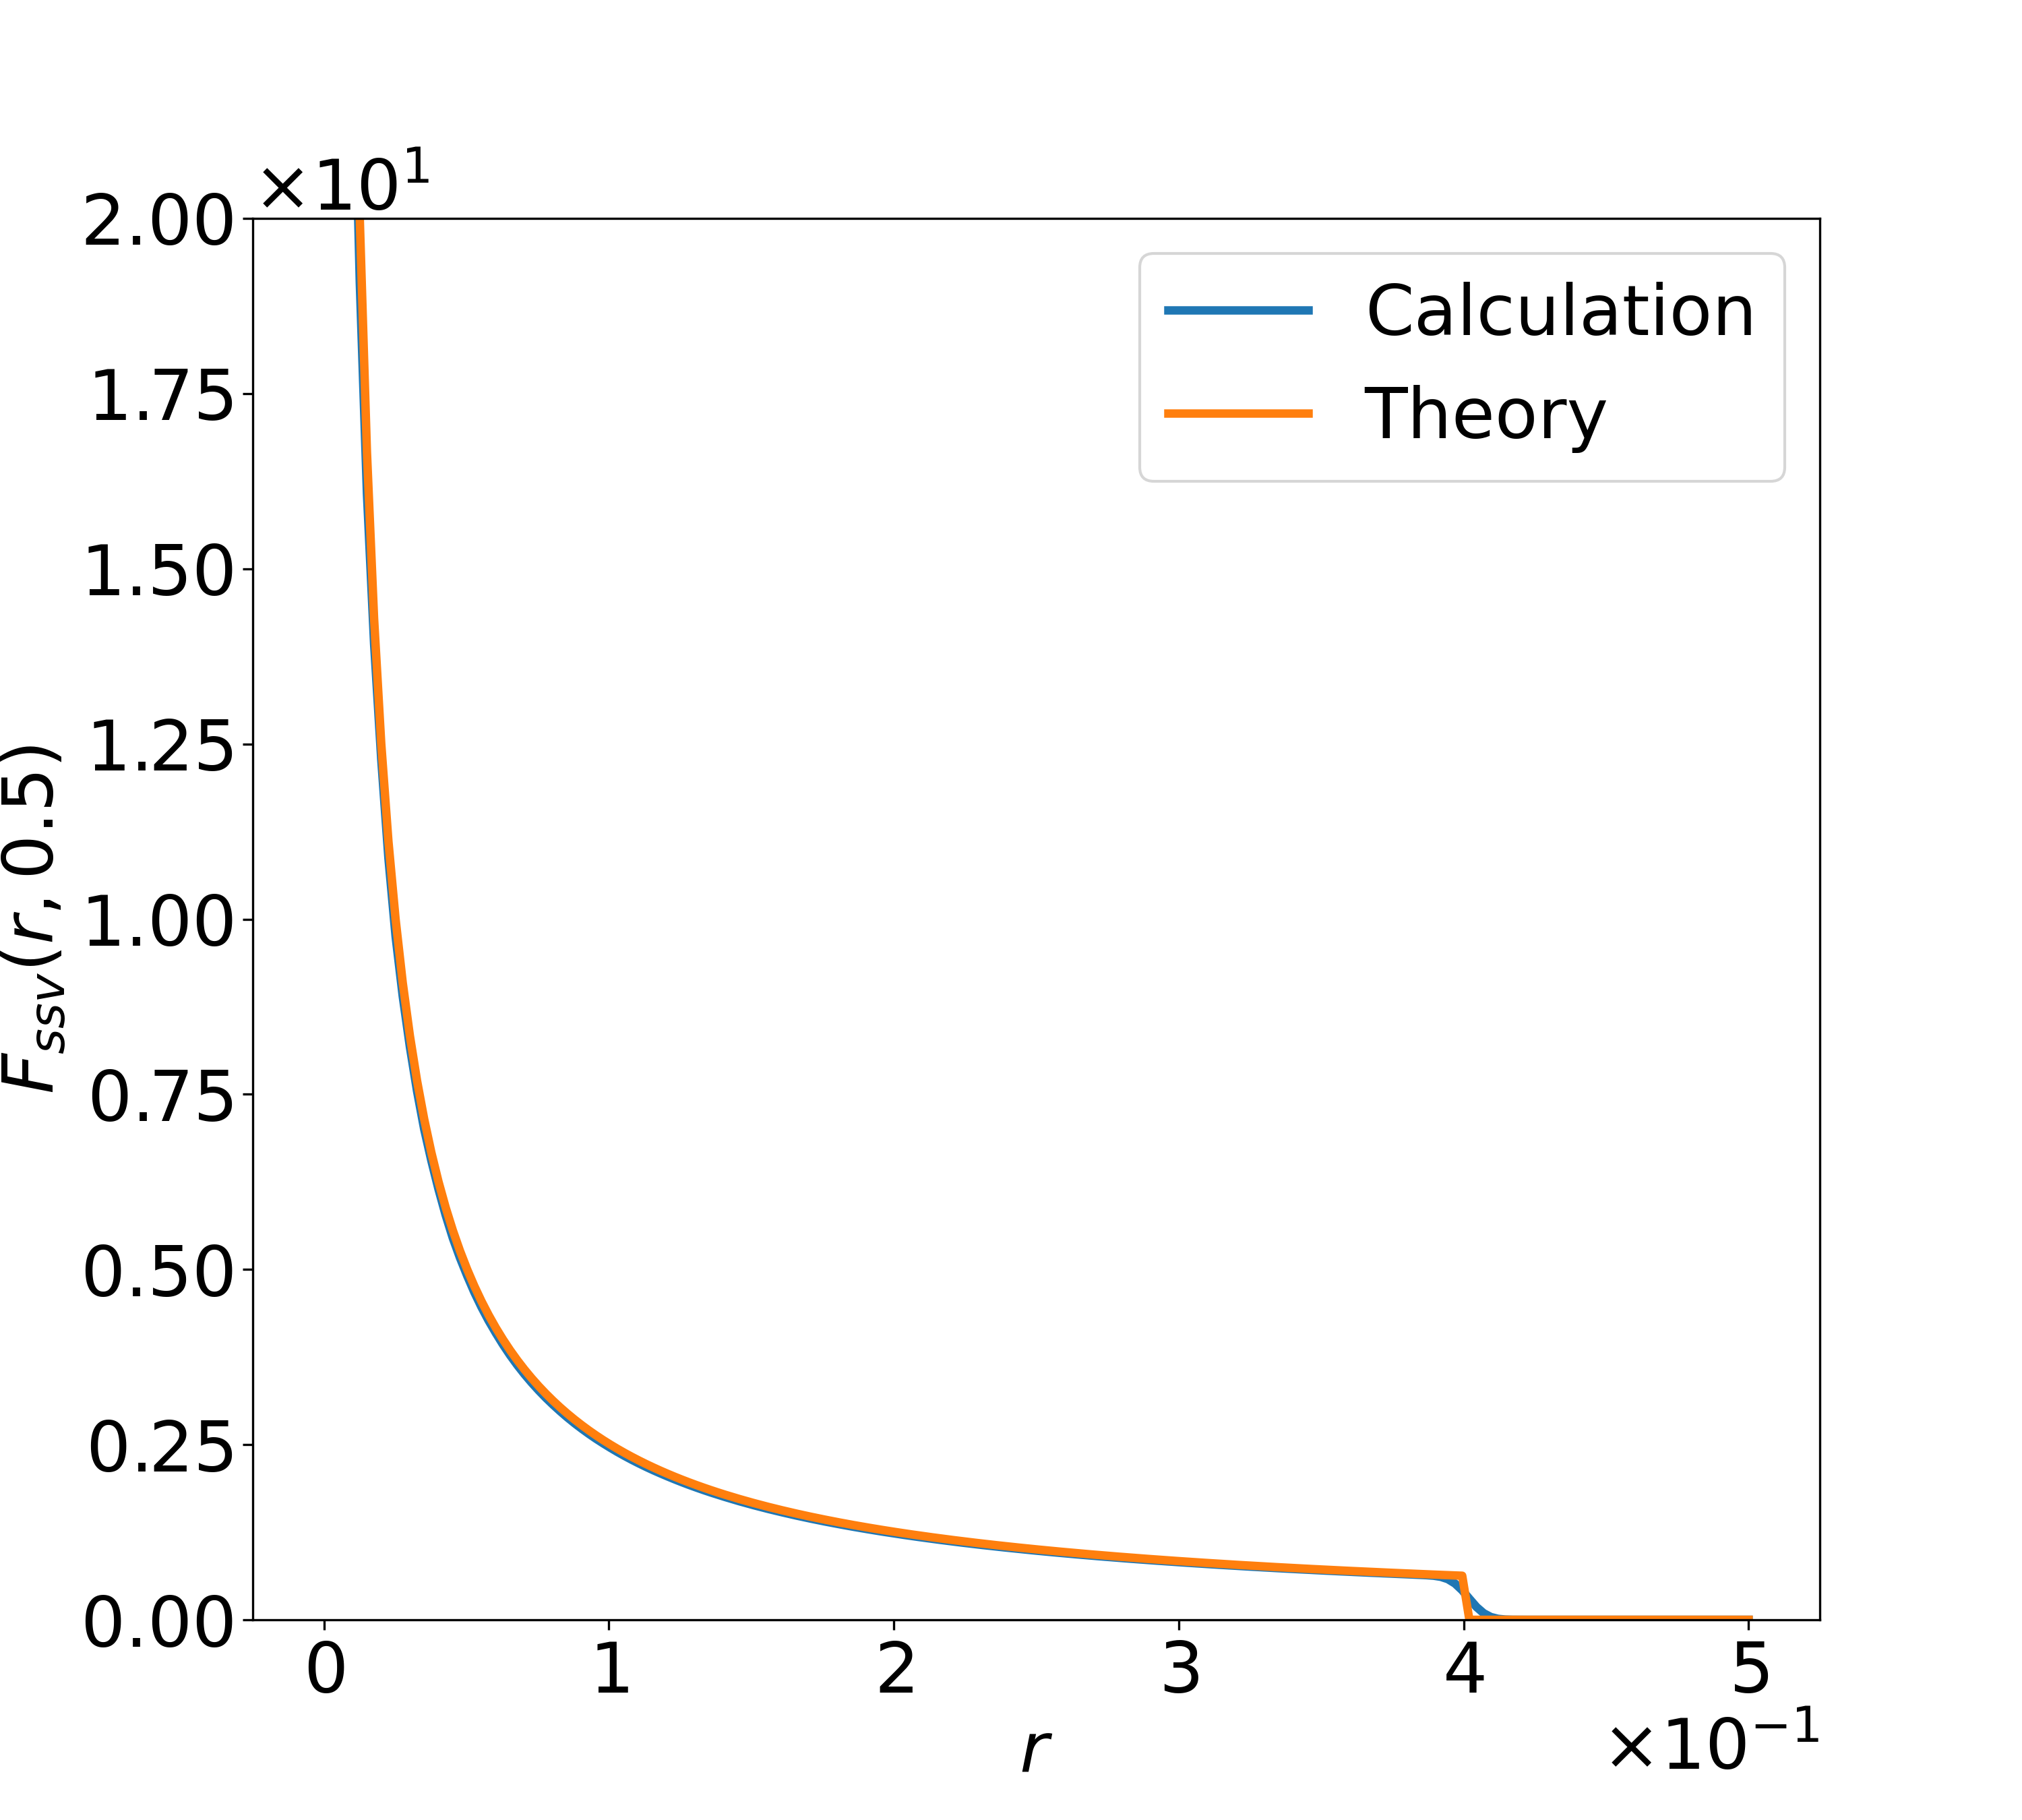
\includegraphics[width=0.45\linewidth]{images/ball-ssv.png}
    \label{fig:balls-ssv}}
  \hfill
  \subfigure[$F_{svv}$]{
    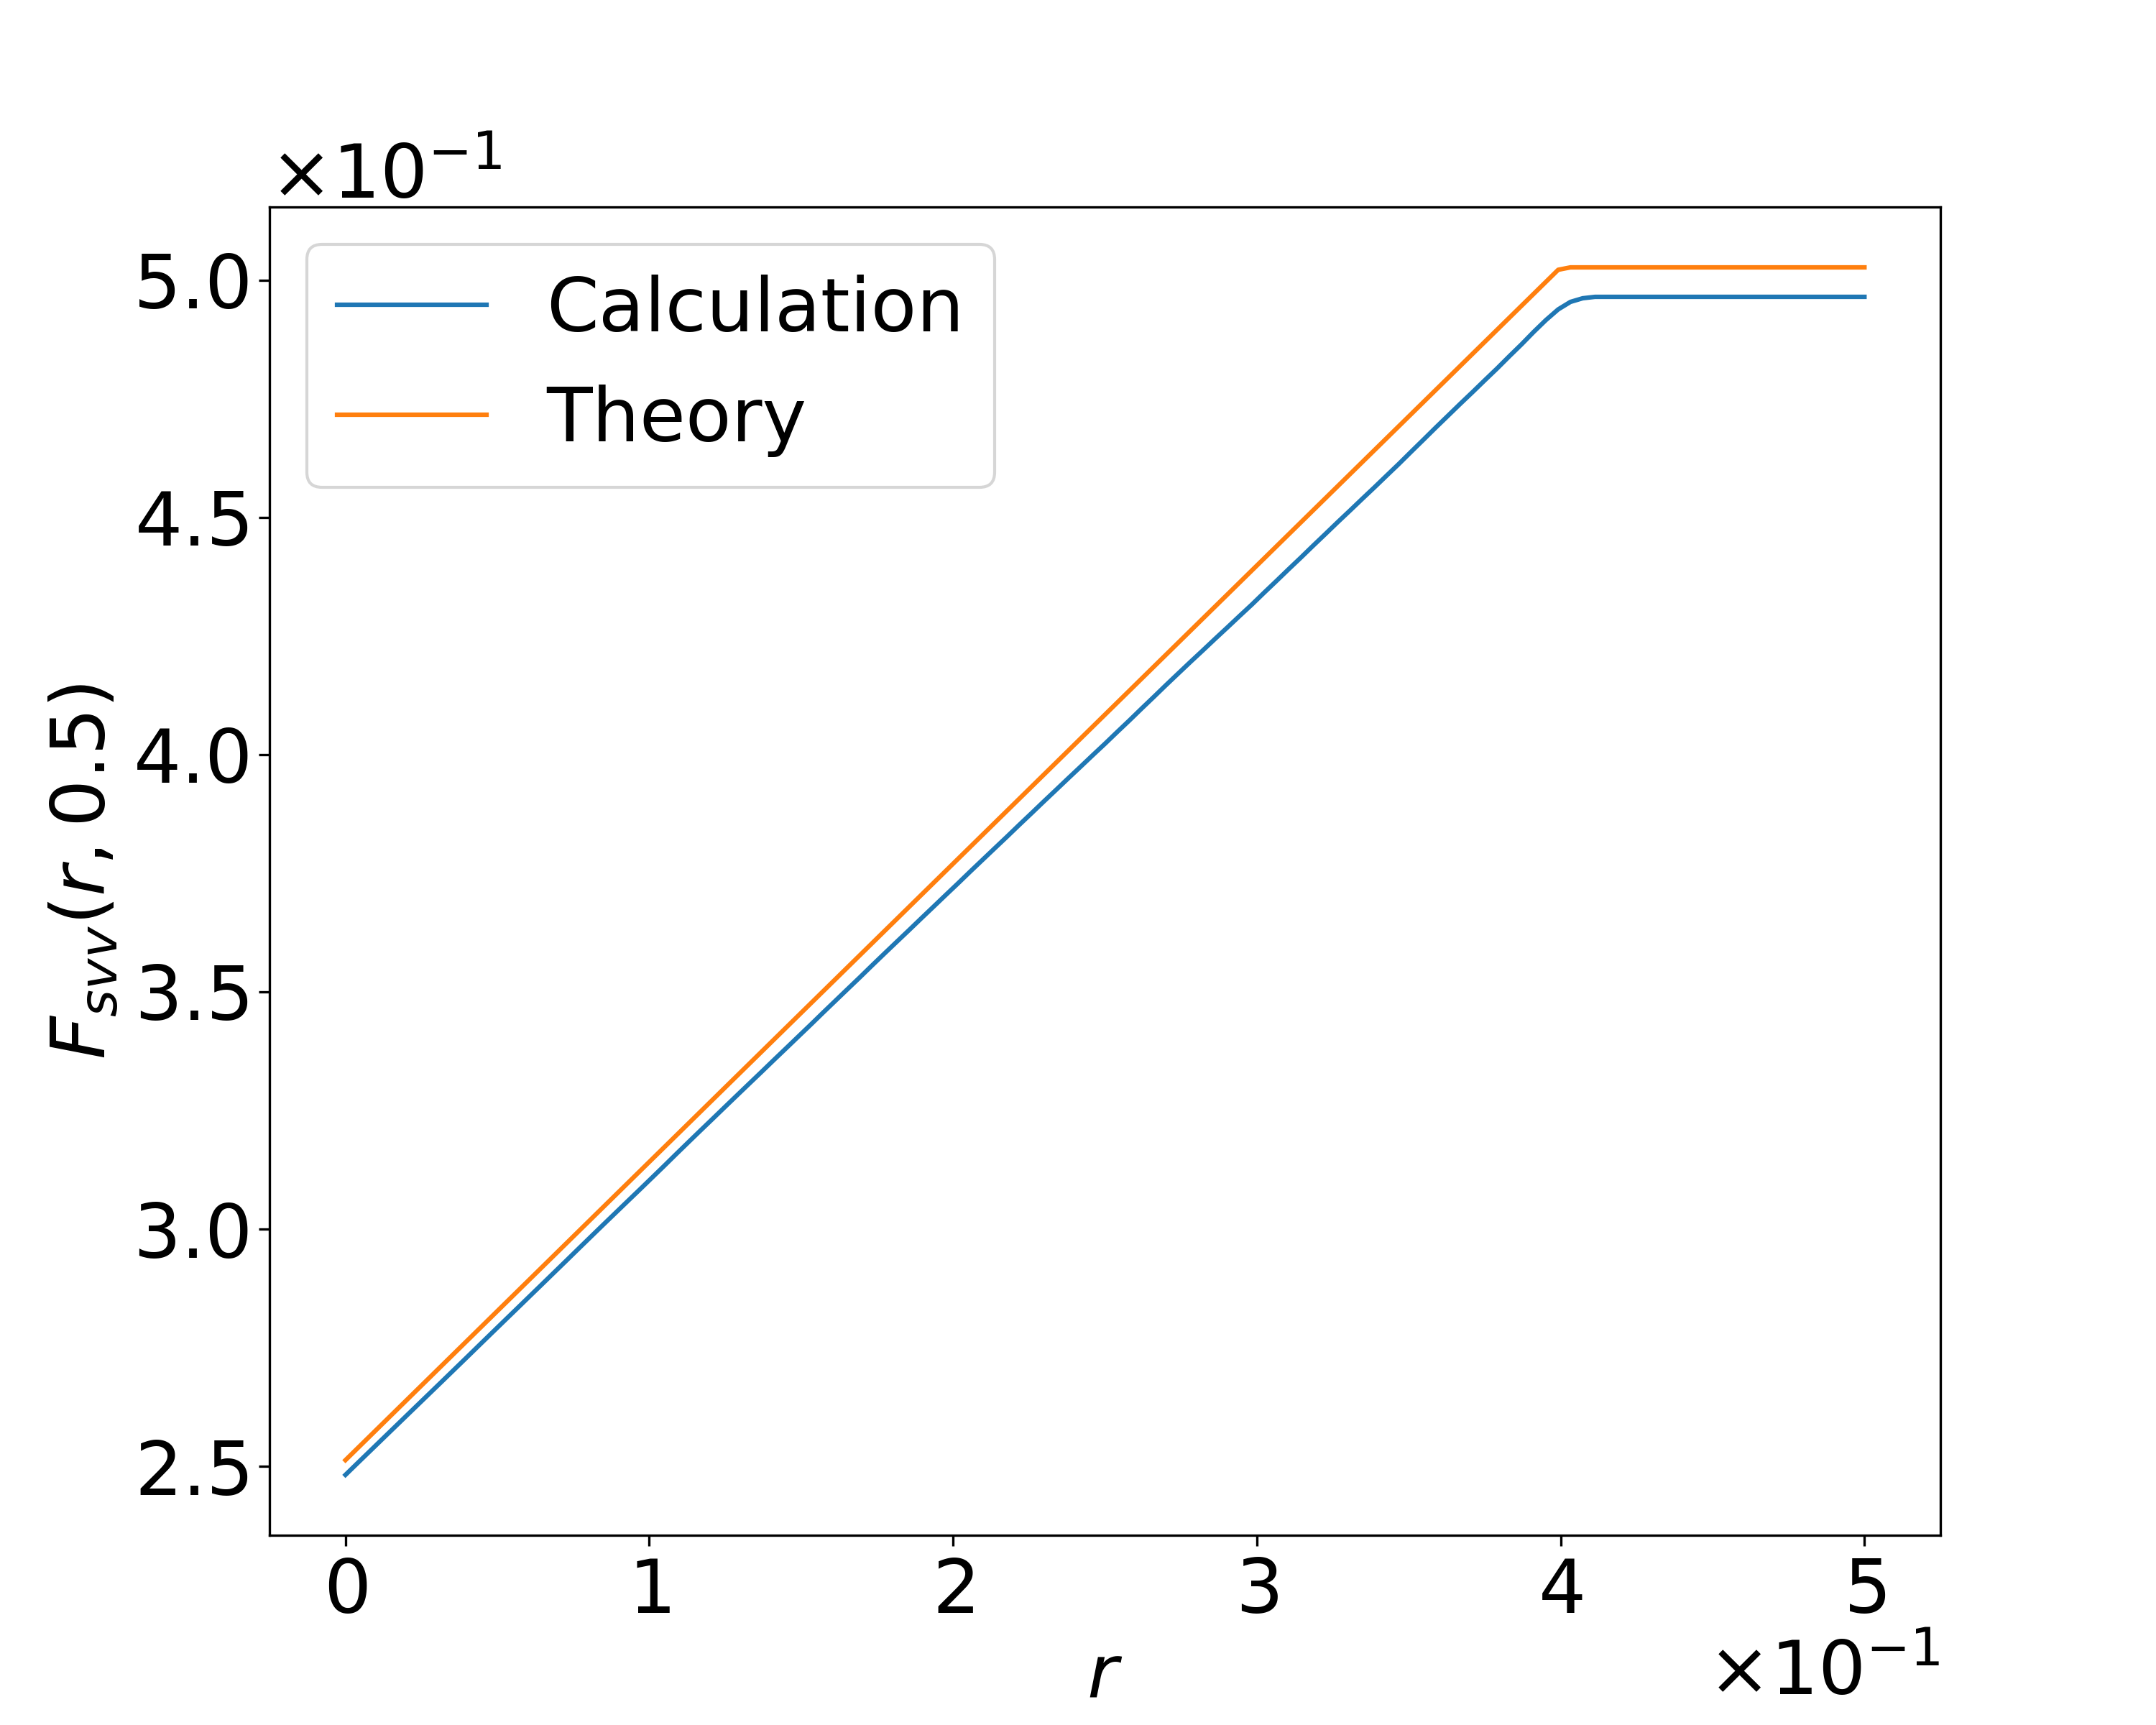
\includegraphics[width=0.45\linewidth]{images/ball-svv.png}
    \label{fig:ball-svv}}
  \caption[]{Comparison of $F_{ssv}$ and $F_{svv}$ functions for a ball with the
    radius $0.2$ with theoretical values.}
  \label{fig:surface-verification}
\end{figure*}

\section{Results}
In this section we compute correlation functions along the plane $XY$ for 2- and
3-dimensional real samples. Table \ref{tab:summary} contains information about
these samples. Note that we compute surface correlation functions only for those
samples for which the criterion $C_{0.5} > 0.97$ holds (the sandstone and the
limestone). Images of the samples are on \cref{fig:samples}. On plots of
correlation functions we provide a family of curves with the first argument of
the correlation function being fixed. For two highly anisotropic samples (the
soil and the shale) we provide heatmaps of $S_3$ correlation function where
anisotropicity can be easily seen. These two samples was preliminary rotated by
$\frac{\pi}{4}$ around the axis $Z$ before calculation of correlation functions.

Correlation functions for the XCT sample of the limestone are on
\cref{fig:sample-limestone-cf}. The plot of $S_3$ function allows us to estimate
porosity of the sample to be $\sim 0.04$ (note, that the curve with $r_1 = 0$ is
actually $S_2$ function). The two-point correlation function reaches plateau at
$r_2 \approx 200\div 225\ \mu m$ which means that two events of finding two
points in the void phase are independent if the points are farther than
$225\ \mu m$ from each other. We see that the sample is a little bit anisotropic
($S_3(0, 225) \approx S_3(150, 0)$). From analysis of $C_3$ function it can be
stated that the sample has clusters of void phase which are $\sim 200\ \mu m$ in
diameter.

Correlation functions for the SEM sample (the sandstone) are on
\cref{fig:sample-sandstone-cf}. Porosity of the sample is $\sim 0.3$ as follows
from the plot of $S_3$ function at $r_1 = 0$. The funcion $S_3(0, r_2)$ reaches
plateau at $r_2 \approx 20\ \mu m$. The sample is highly anisotropic (elongated
along the ordinate). The samples has clusters which are $\sim 45\ \mu m$ in
diameter.

Heatmaps of $S_3$ for the two highly anisotropic samples can be seen on
\cref{fig:heatmaps}. Anisotropicity of the both samples can be seen as a slower
decay of $S_3$ in one of the directions. Additionally, it can be observed that
elongated clusters of the void phase in the sample of soil are parallel to each
other and have a regular spacing about $50 \mu m$.

\begin{table}[!htp]
  \centering
  \begin{tabular}{|c|c|c|c|c|}
    \hline
    Sample name & Image type & Dimensions (pixels) & Image resolution ($\mu m$) & $C_{0.5}$\\
    \hline
    Limestone & XCT &  $600 \times 600 \times 600$ & 3.02 & 0.9712 \\
    Soil & XCT & $160 \times 160 \times 160$ & 2.25 & 0.9210 \\
    Shale & XCT & $160 \times 160 \times 160$ & 2.25 & 0.8912 \\
    Sandstone & SEM &  $1280 \times 869$ & 0.10 & 0.9703 \\
    \hline
  \end{tabular}
  \caption{Summary of samples used for calculation of correlation functions.}
  \label{tab:summary}
\end{table}

\begin{figure*}[tp]
  \centering
  \subfigure[Limestone]{
    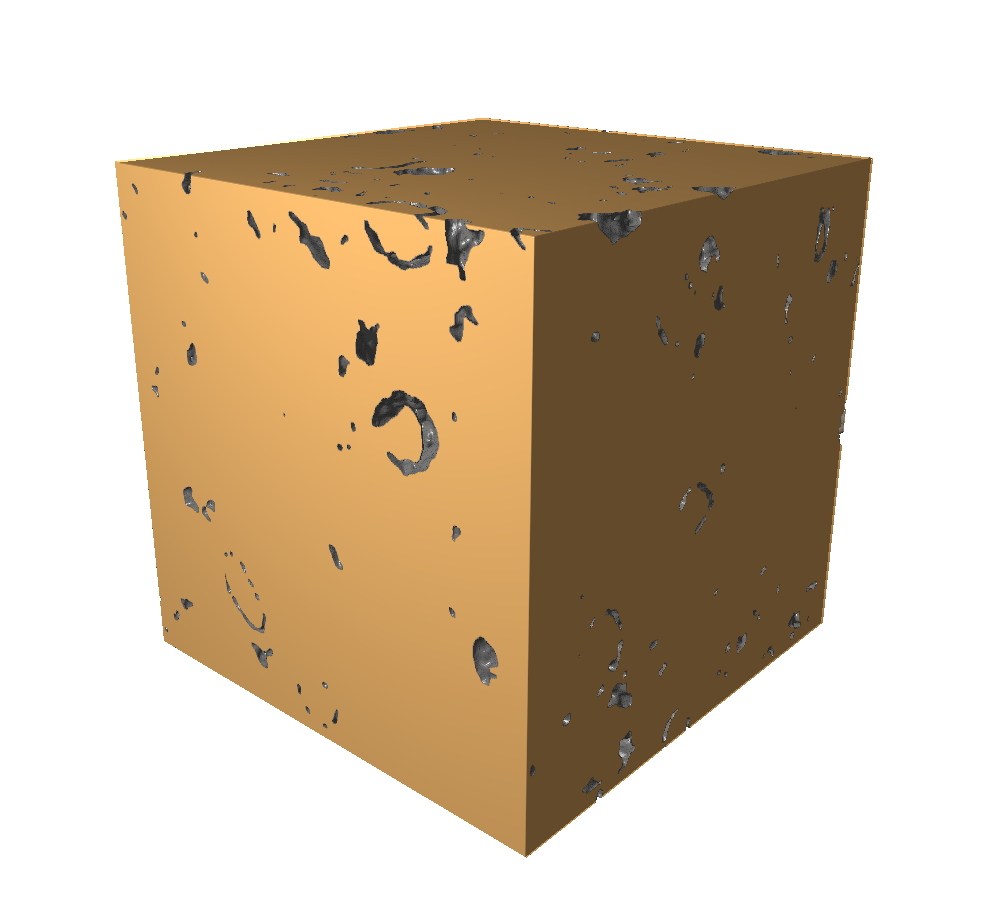
\includegraphics[width=0.45\linewidth]{images/carb.png}
    \label{fig:sample-limestone}}
  \hfill
  \subfigure[Sandstone (different clusters of void phase are shown in color)]{
    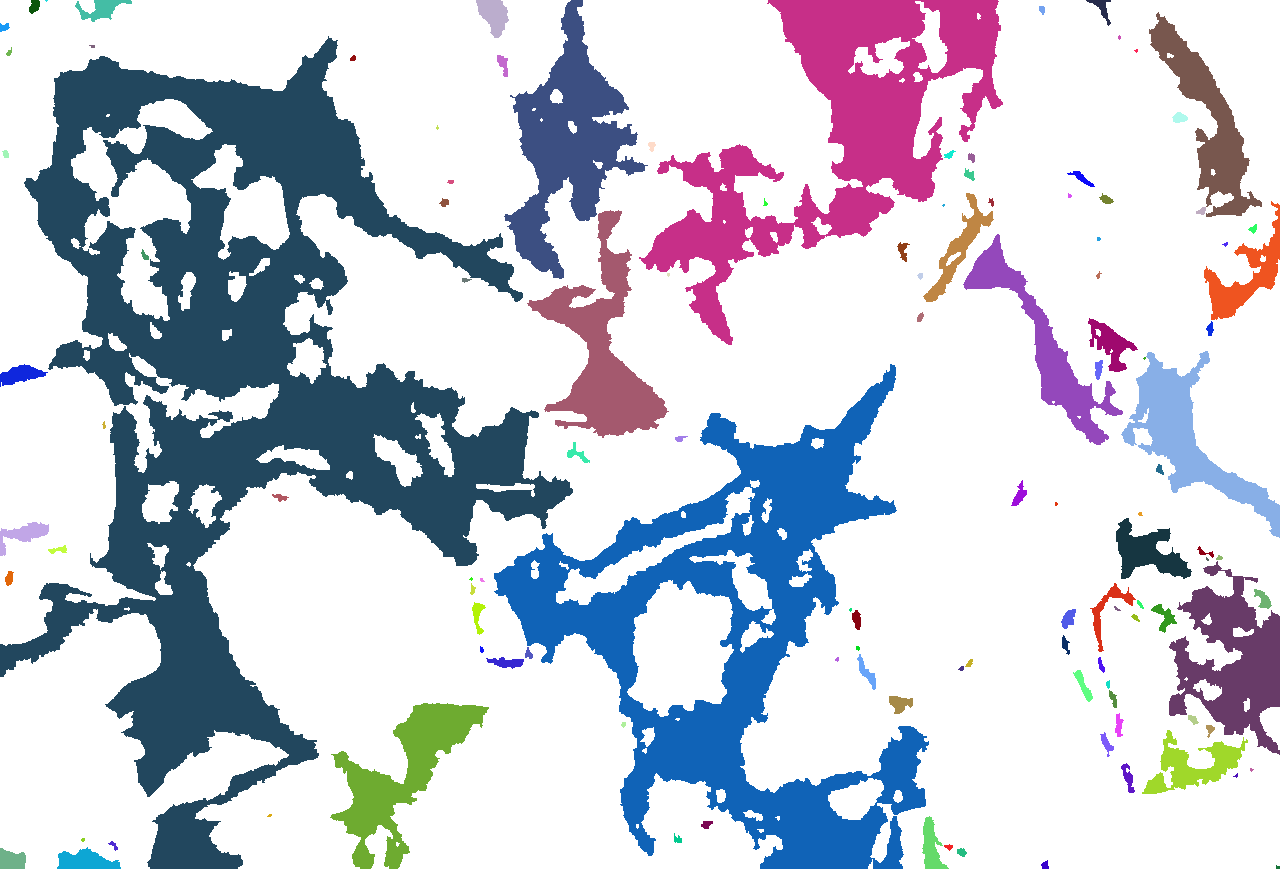
\includegraphics[width=0.45\linewidth, frame]{images/sandstone1.png}
    \label{fig:sample-sandstone}}
  \vskip\baselineskip
  \subfigure[Soil]{
    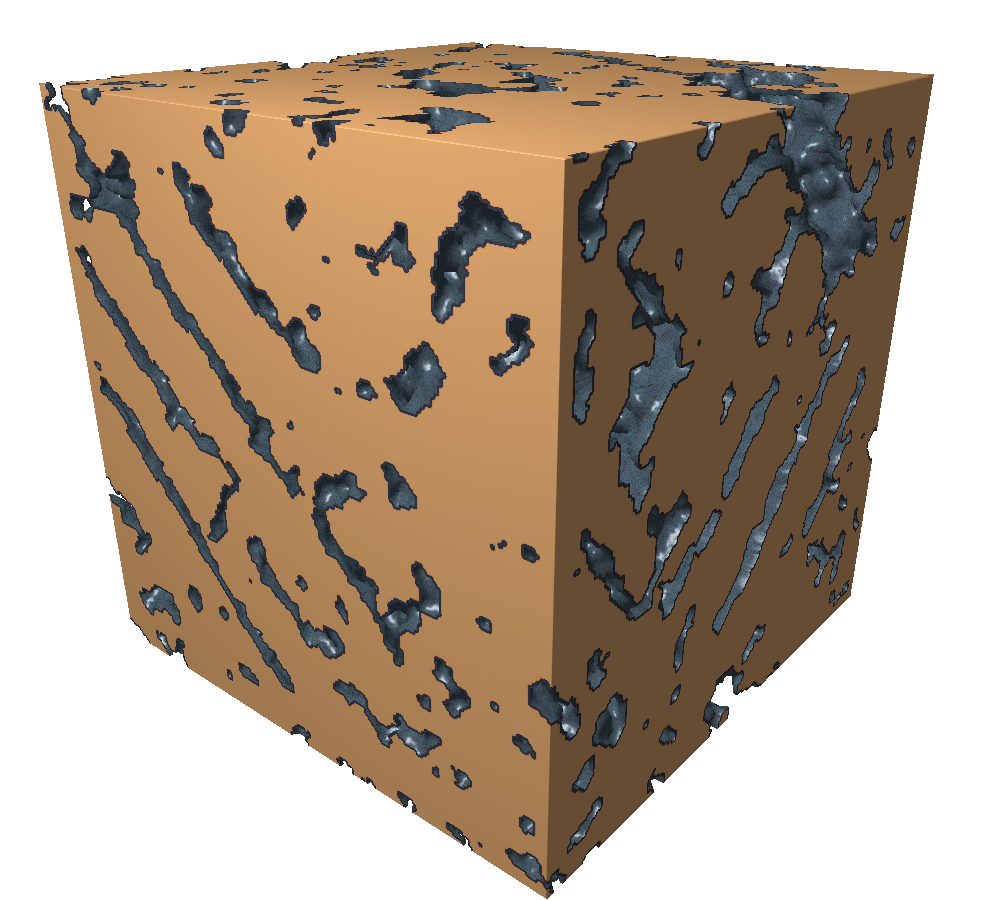
\includegraphics[width=0.45\linewidth]{images/soil.png}
    \label{fig:sample-soil}}
  \hfill
  \subfigure[Shale]{
    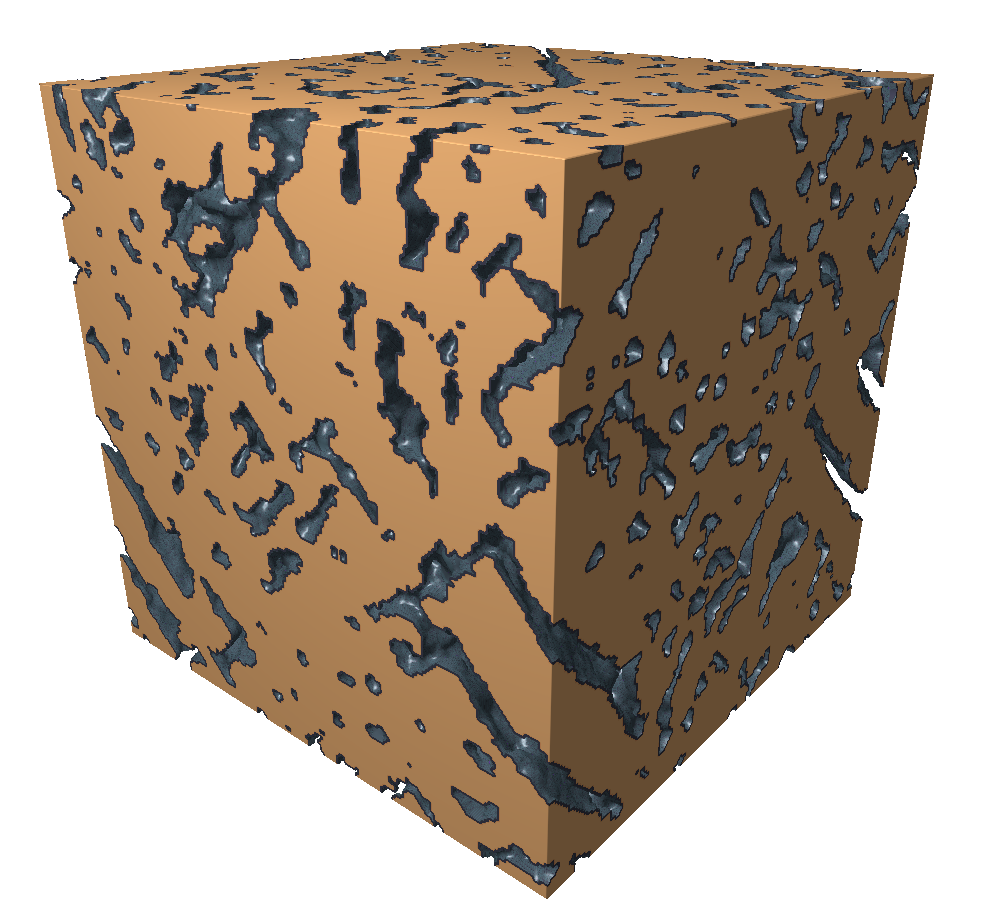
\includegraphics[width=0.45\linewidth]{images/shale.png}
    \label{fig:sample-shale}}
  \caption[]{Images of samples used for calculation of higher-order correlation
    functions.}
  \label{fig:samples}
\end{figure*}

\begin{figure}[tp]
  \centering
  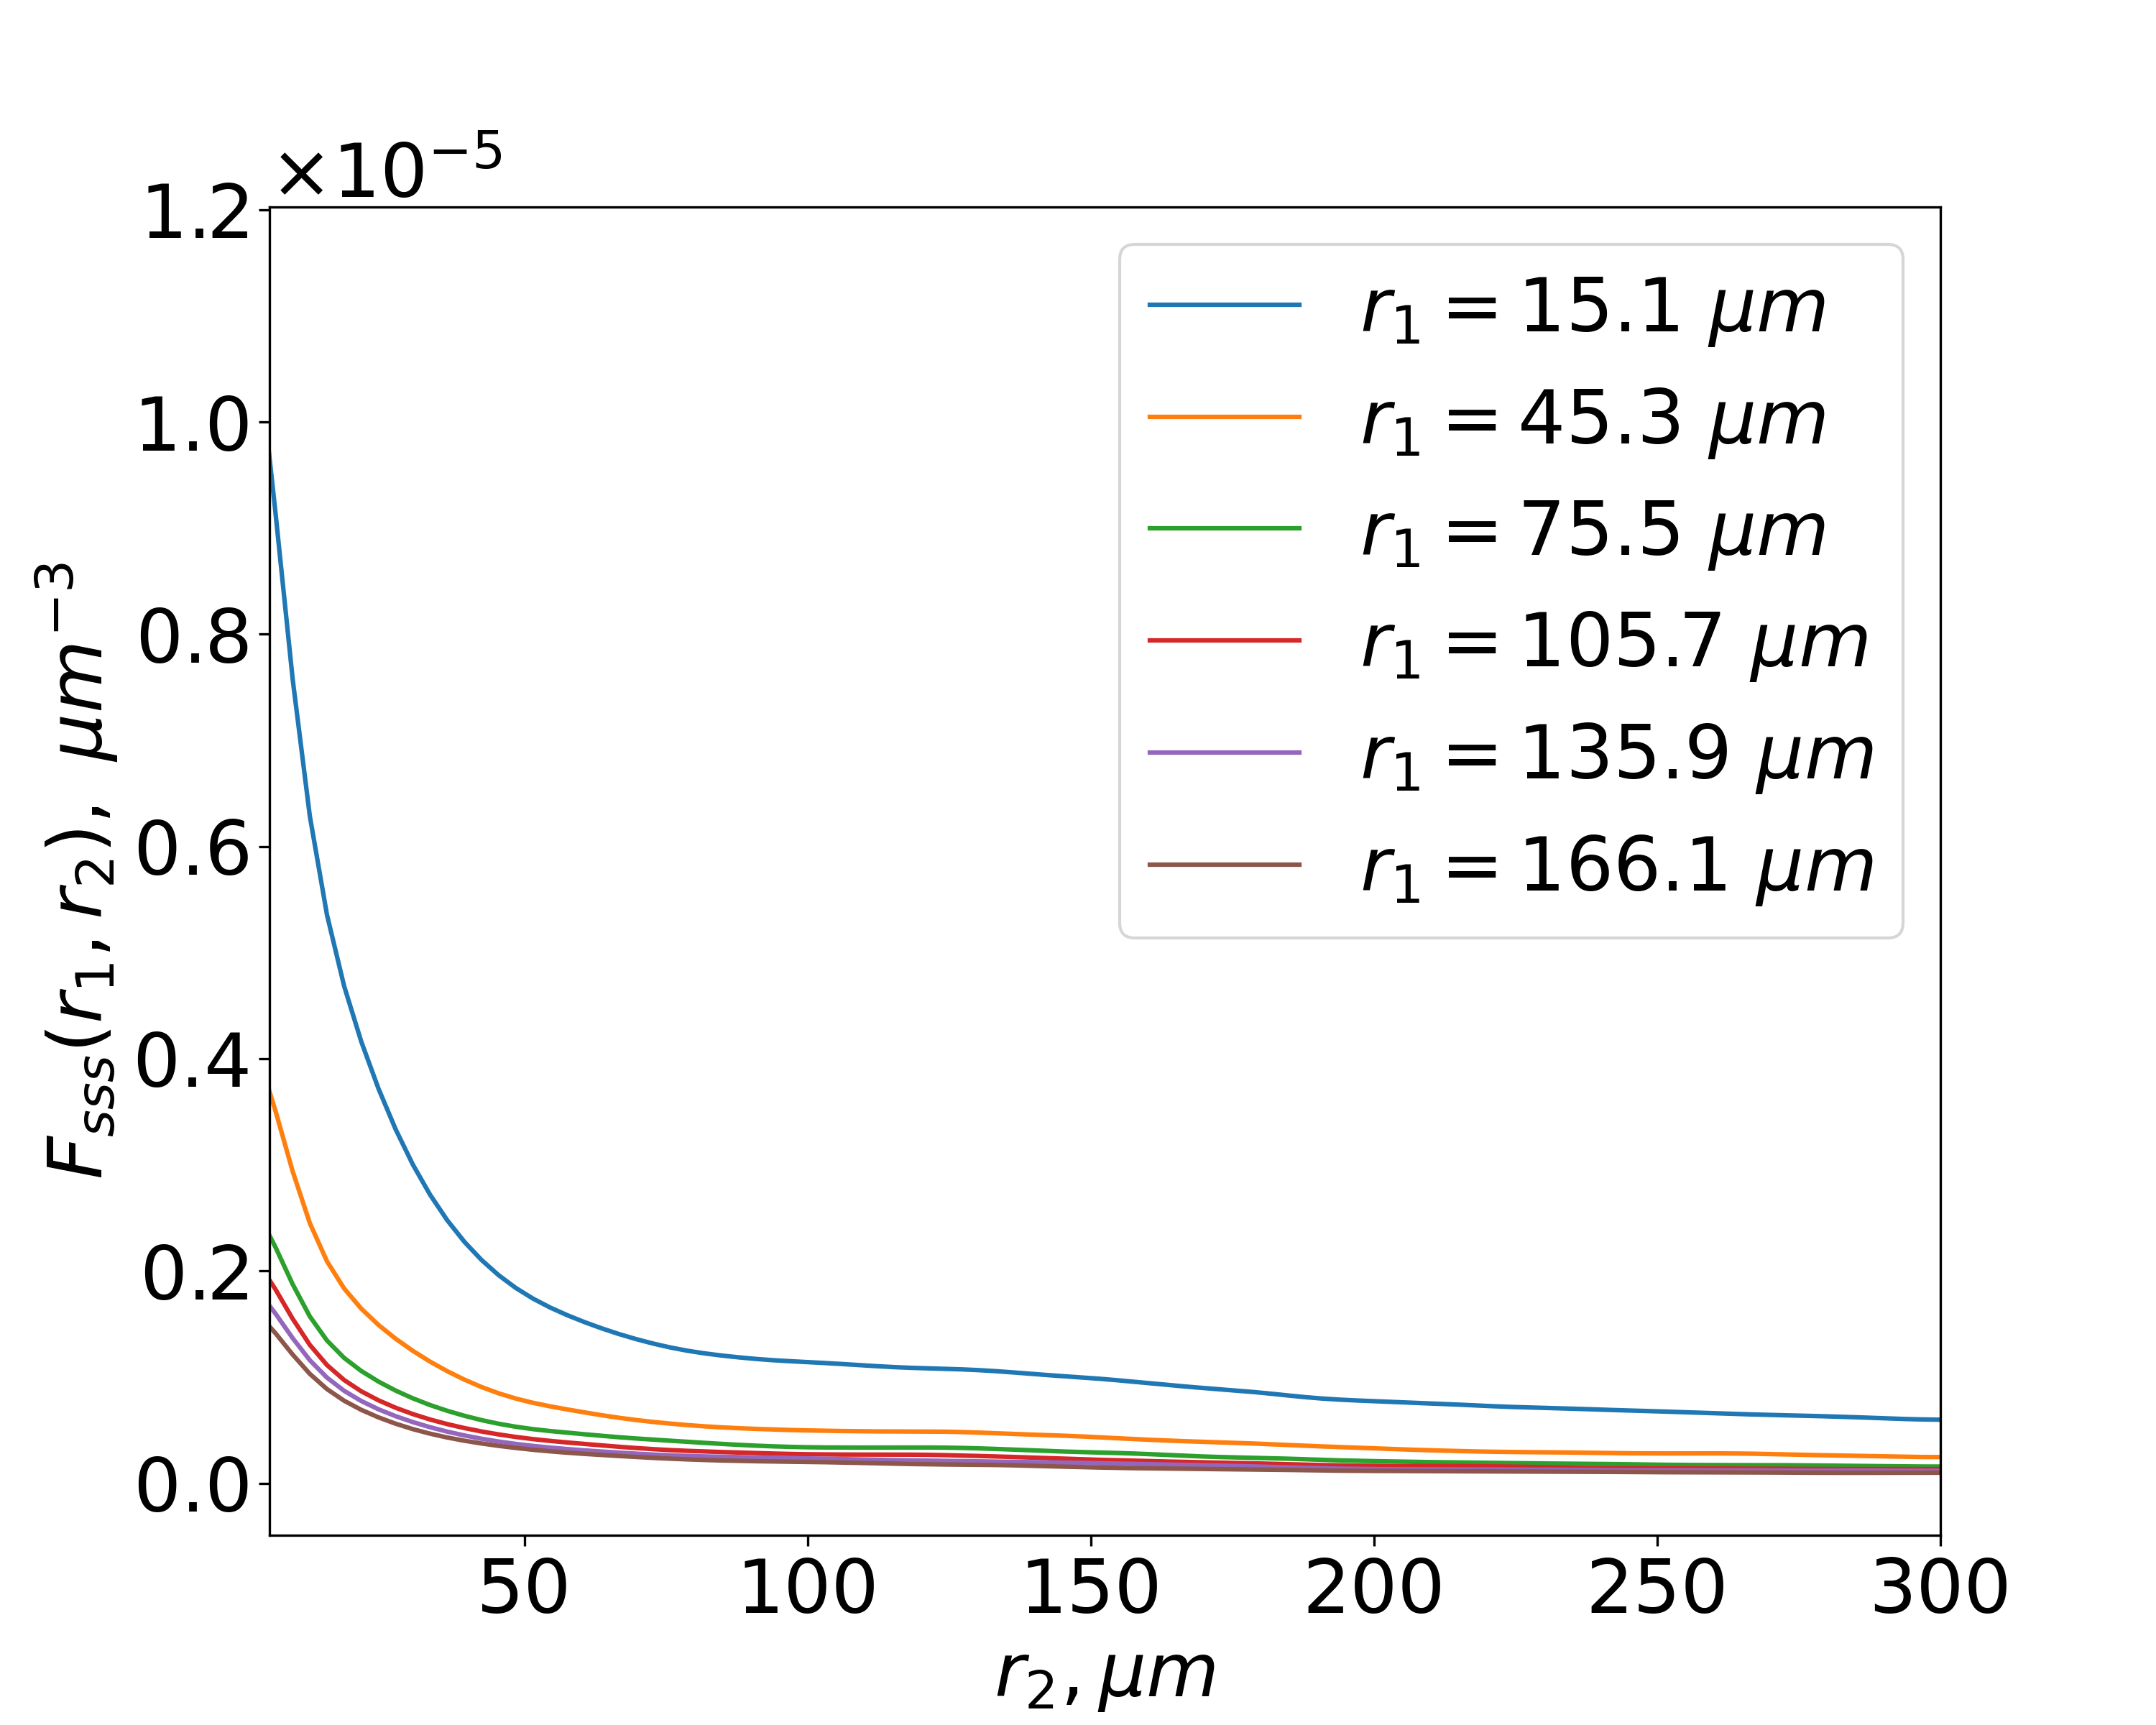
\includegraphics[width=0.45\linewidth]{images/carb.npy-surf3.png}
  \hfill
  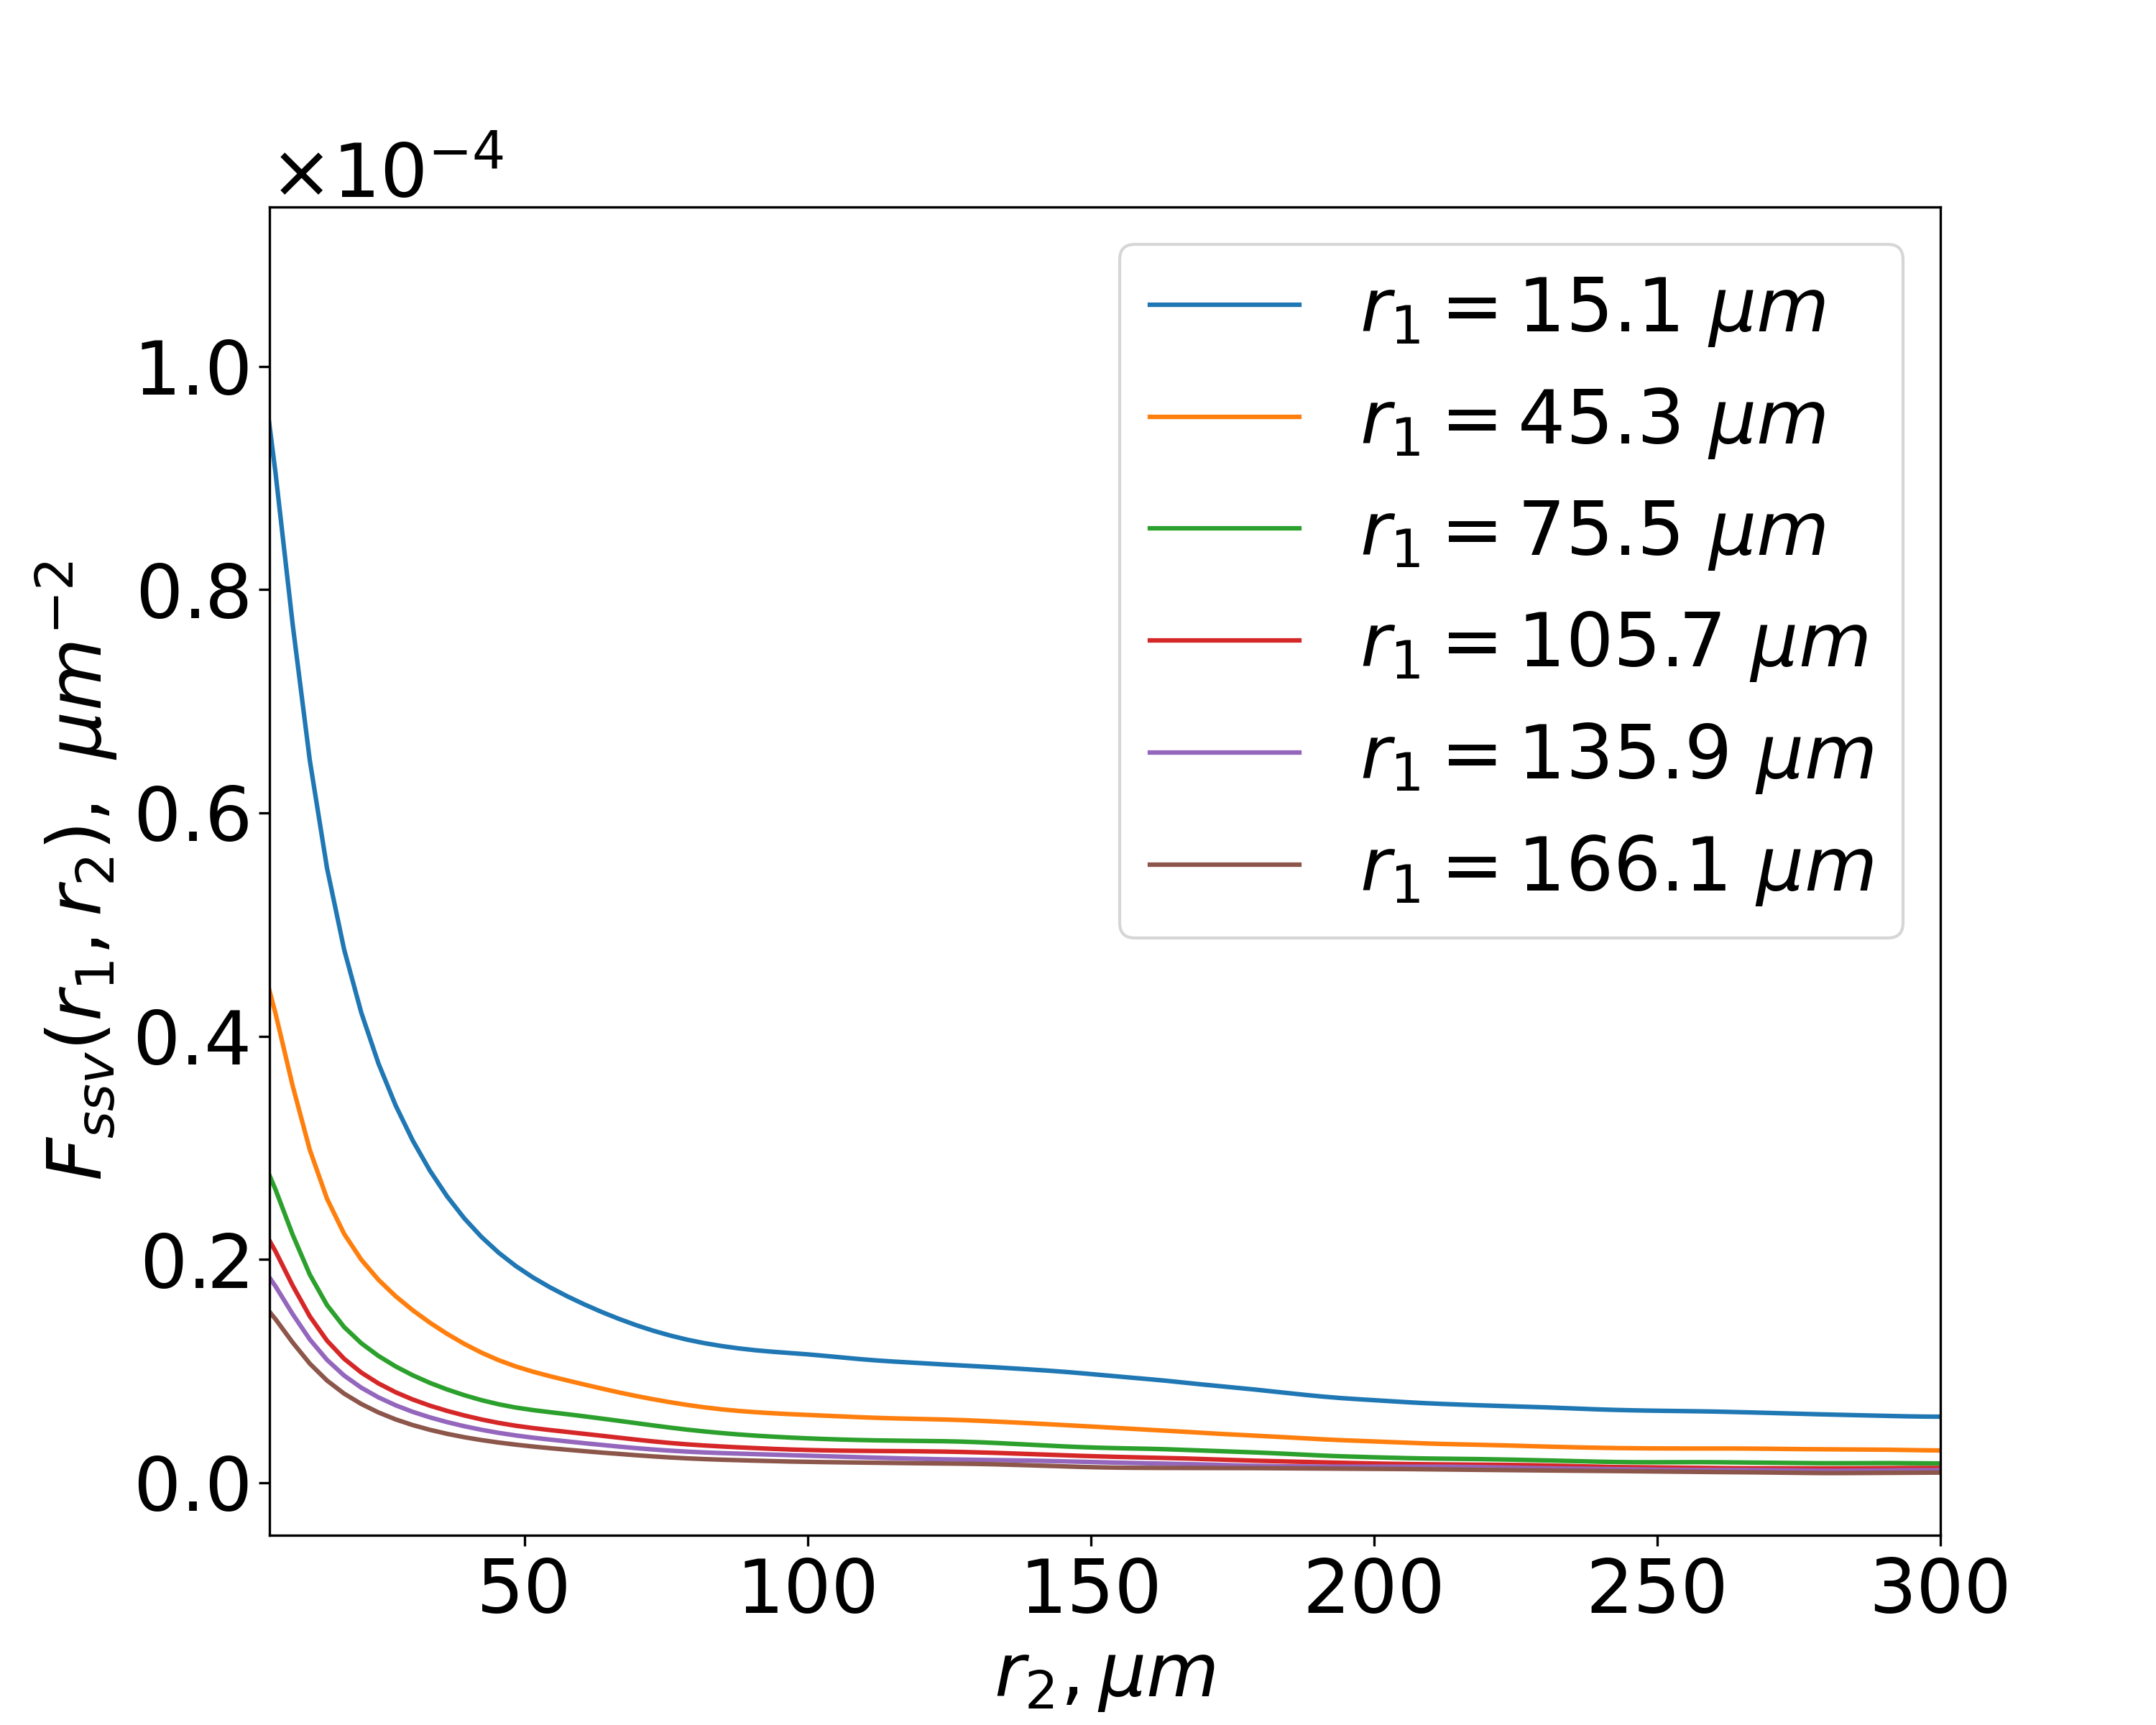
\includegraphics[width=0.45\linewidth]{images/carb.npy-surf2void.png}
  \vskip\baselineskip
  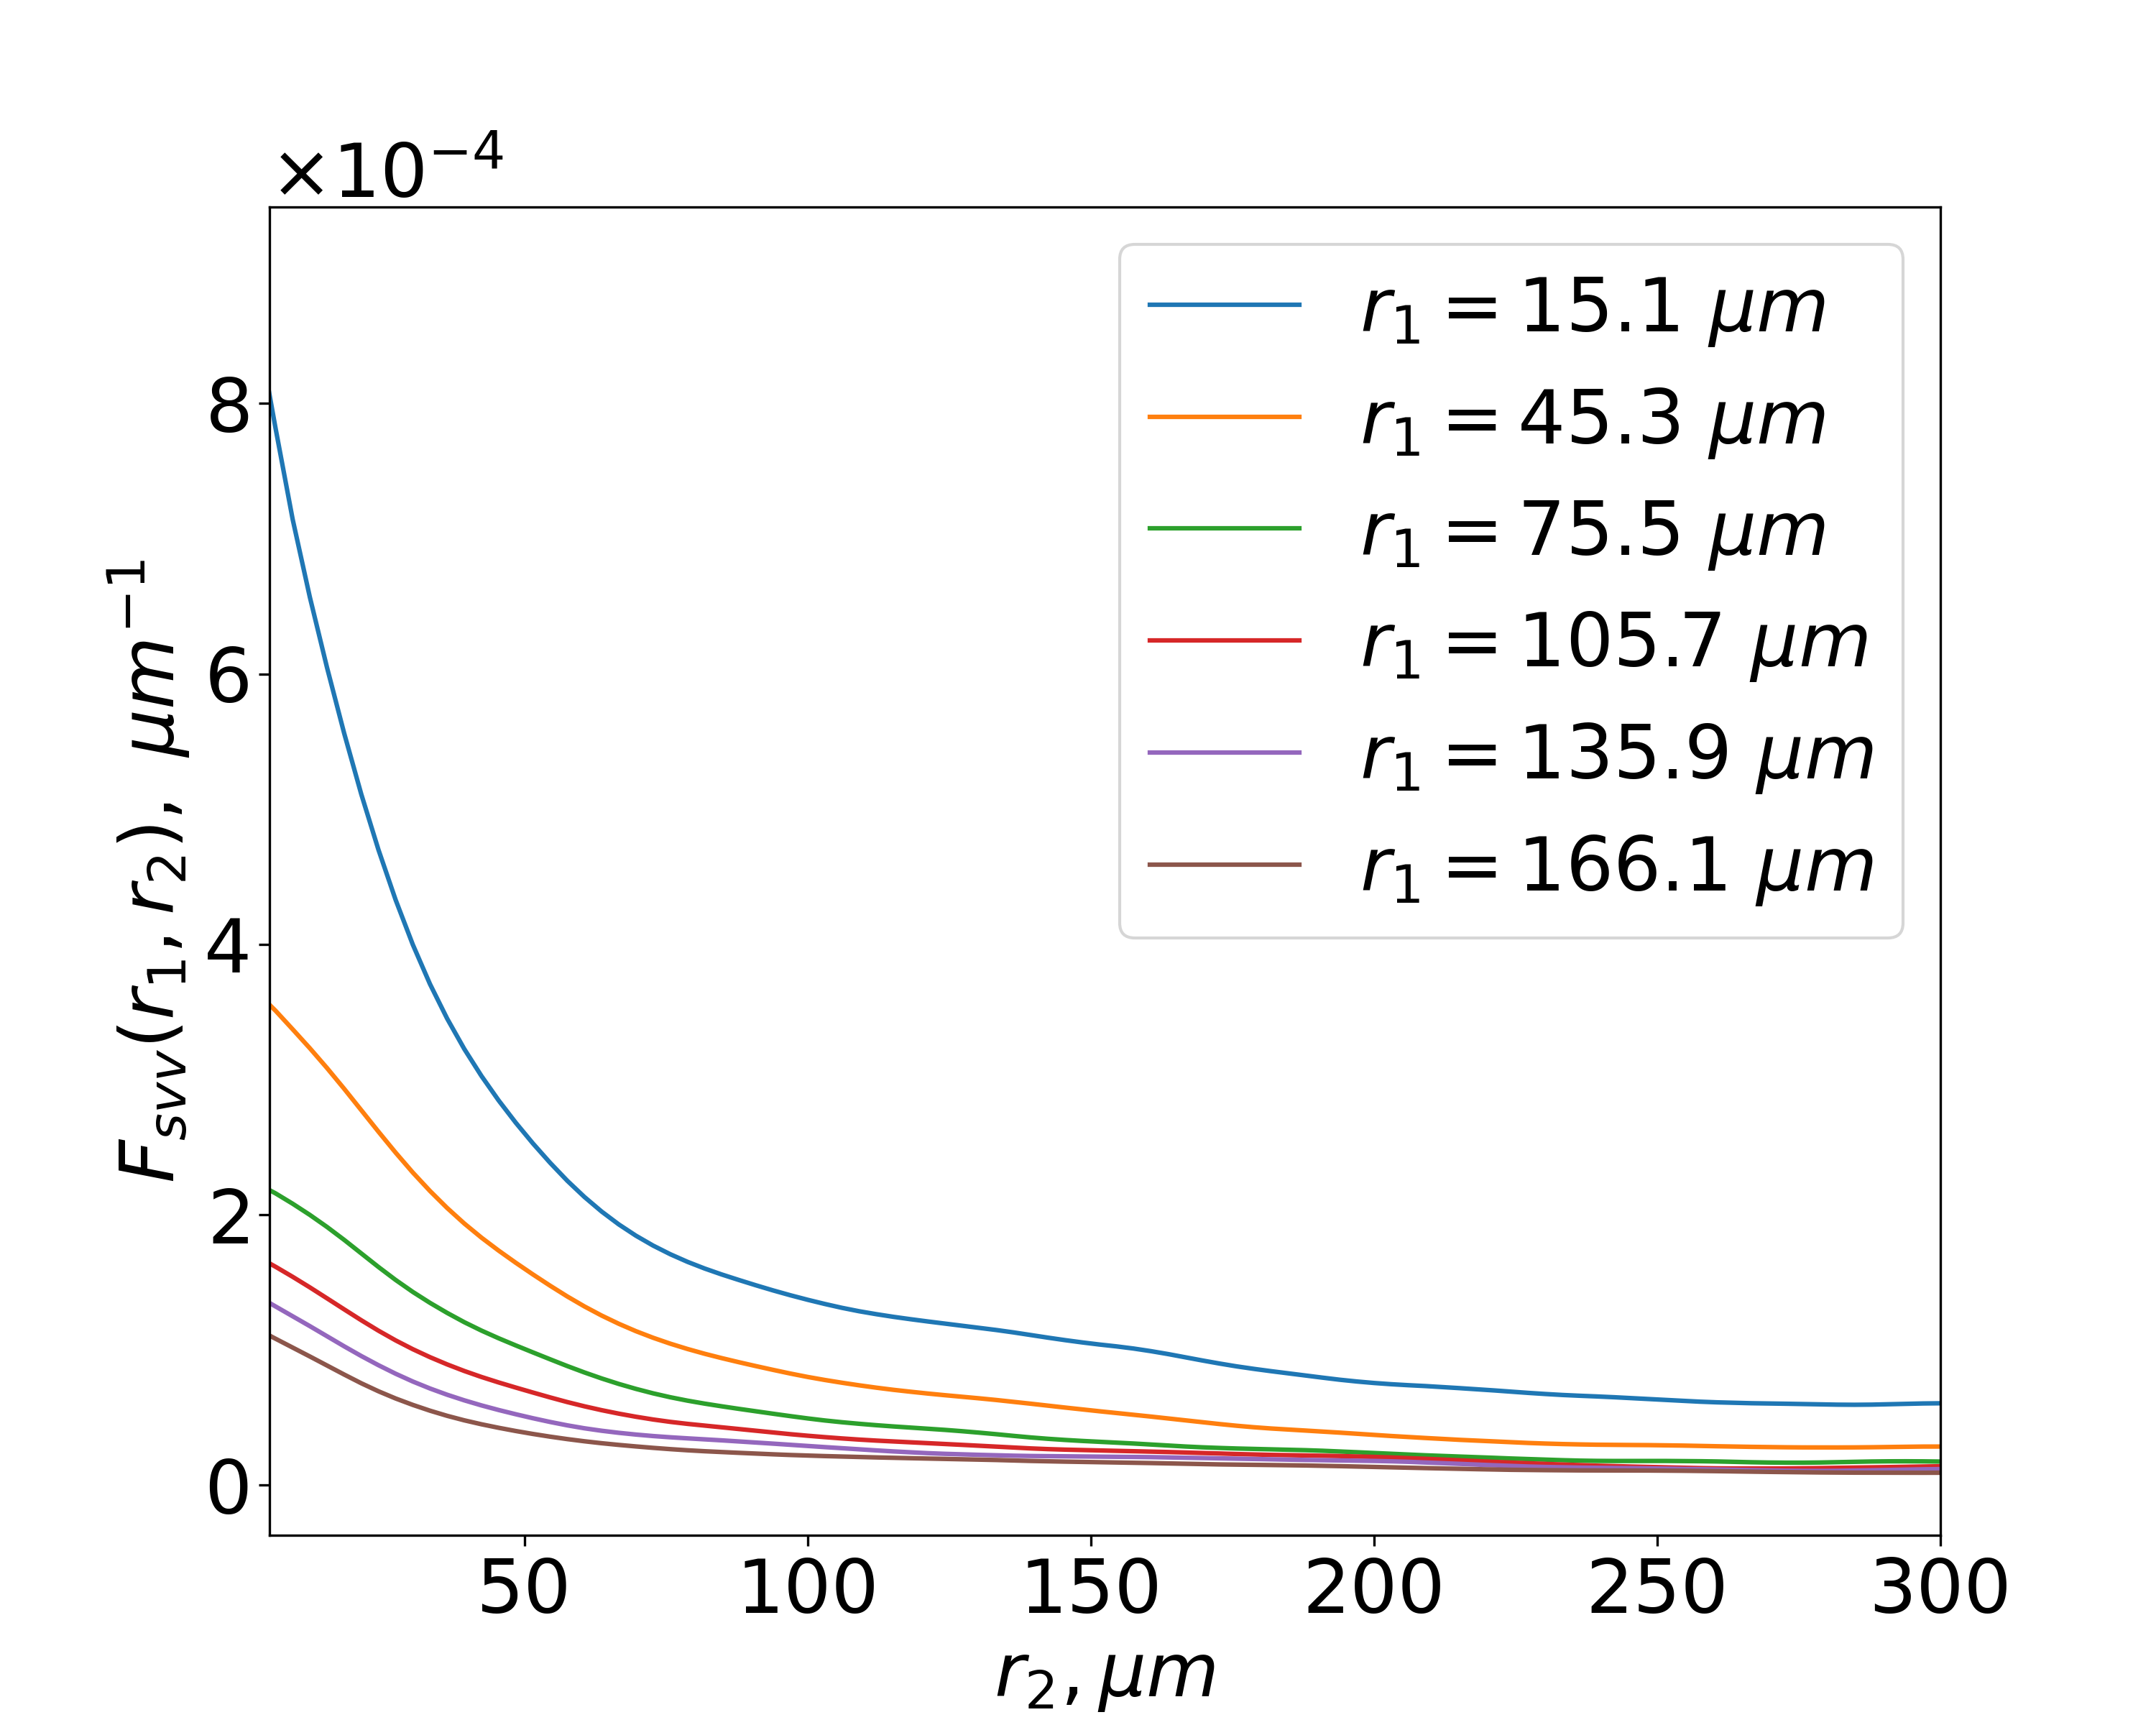
\includegraphics[width=0.45\linewidth]{images/carb.npy-surfvoid2.png}
  \hfill
  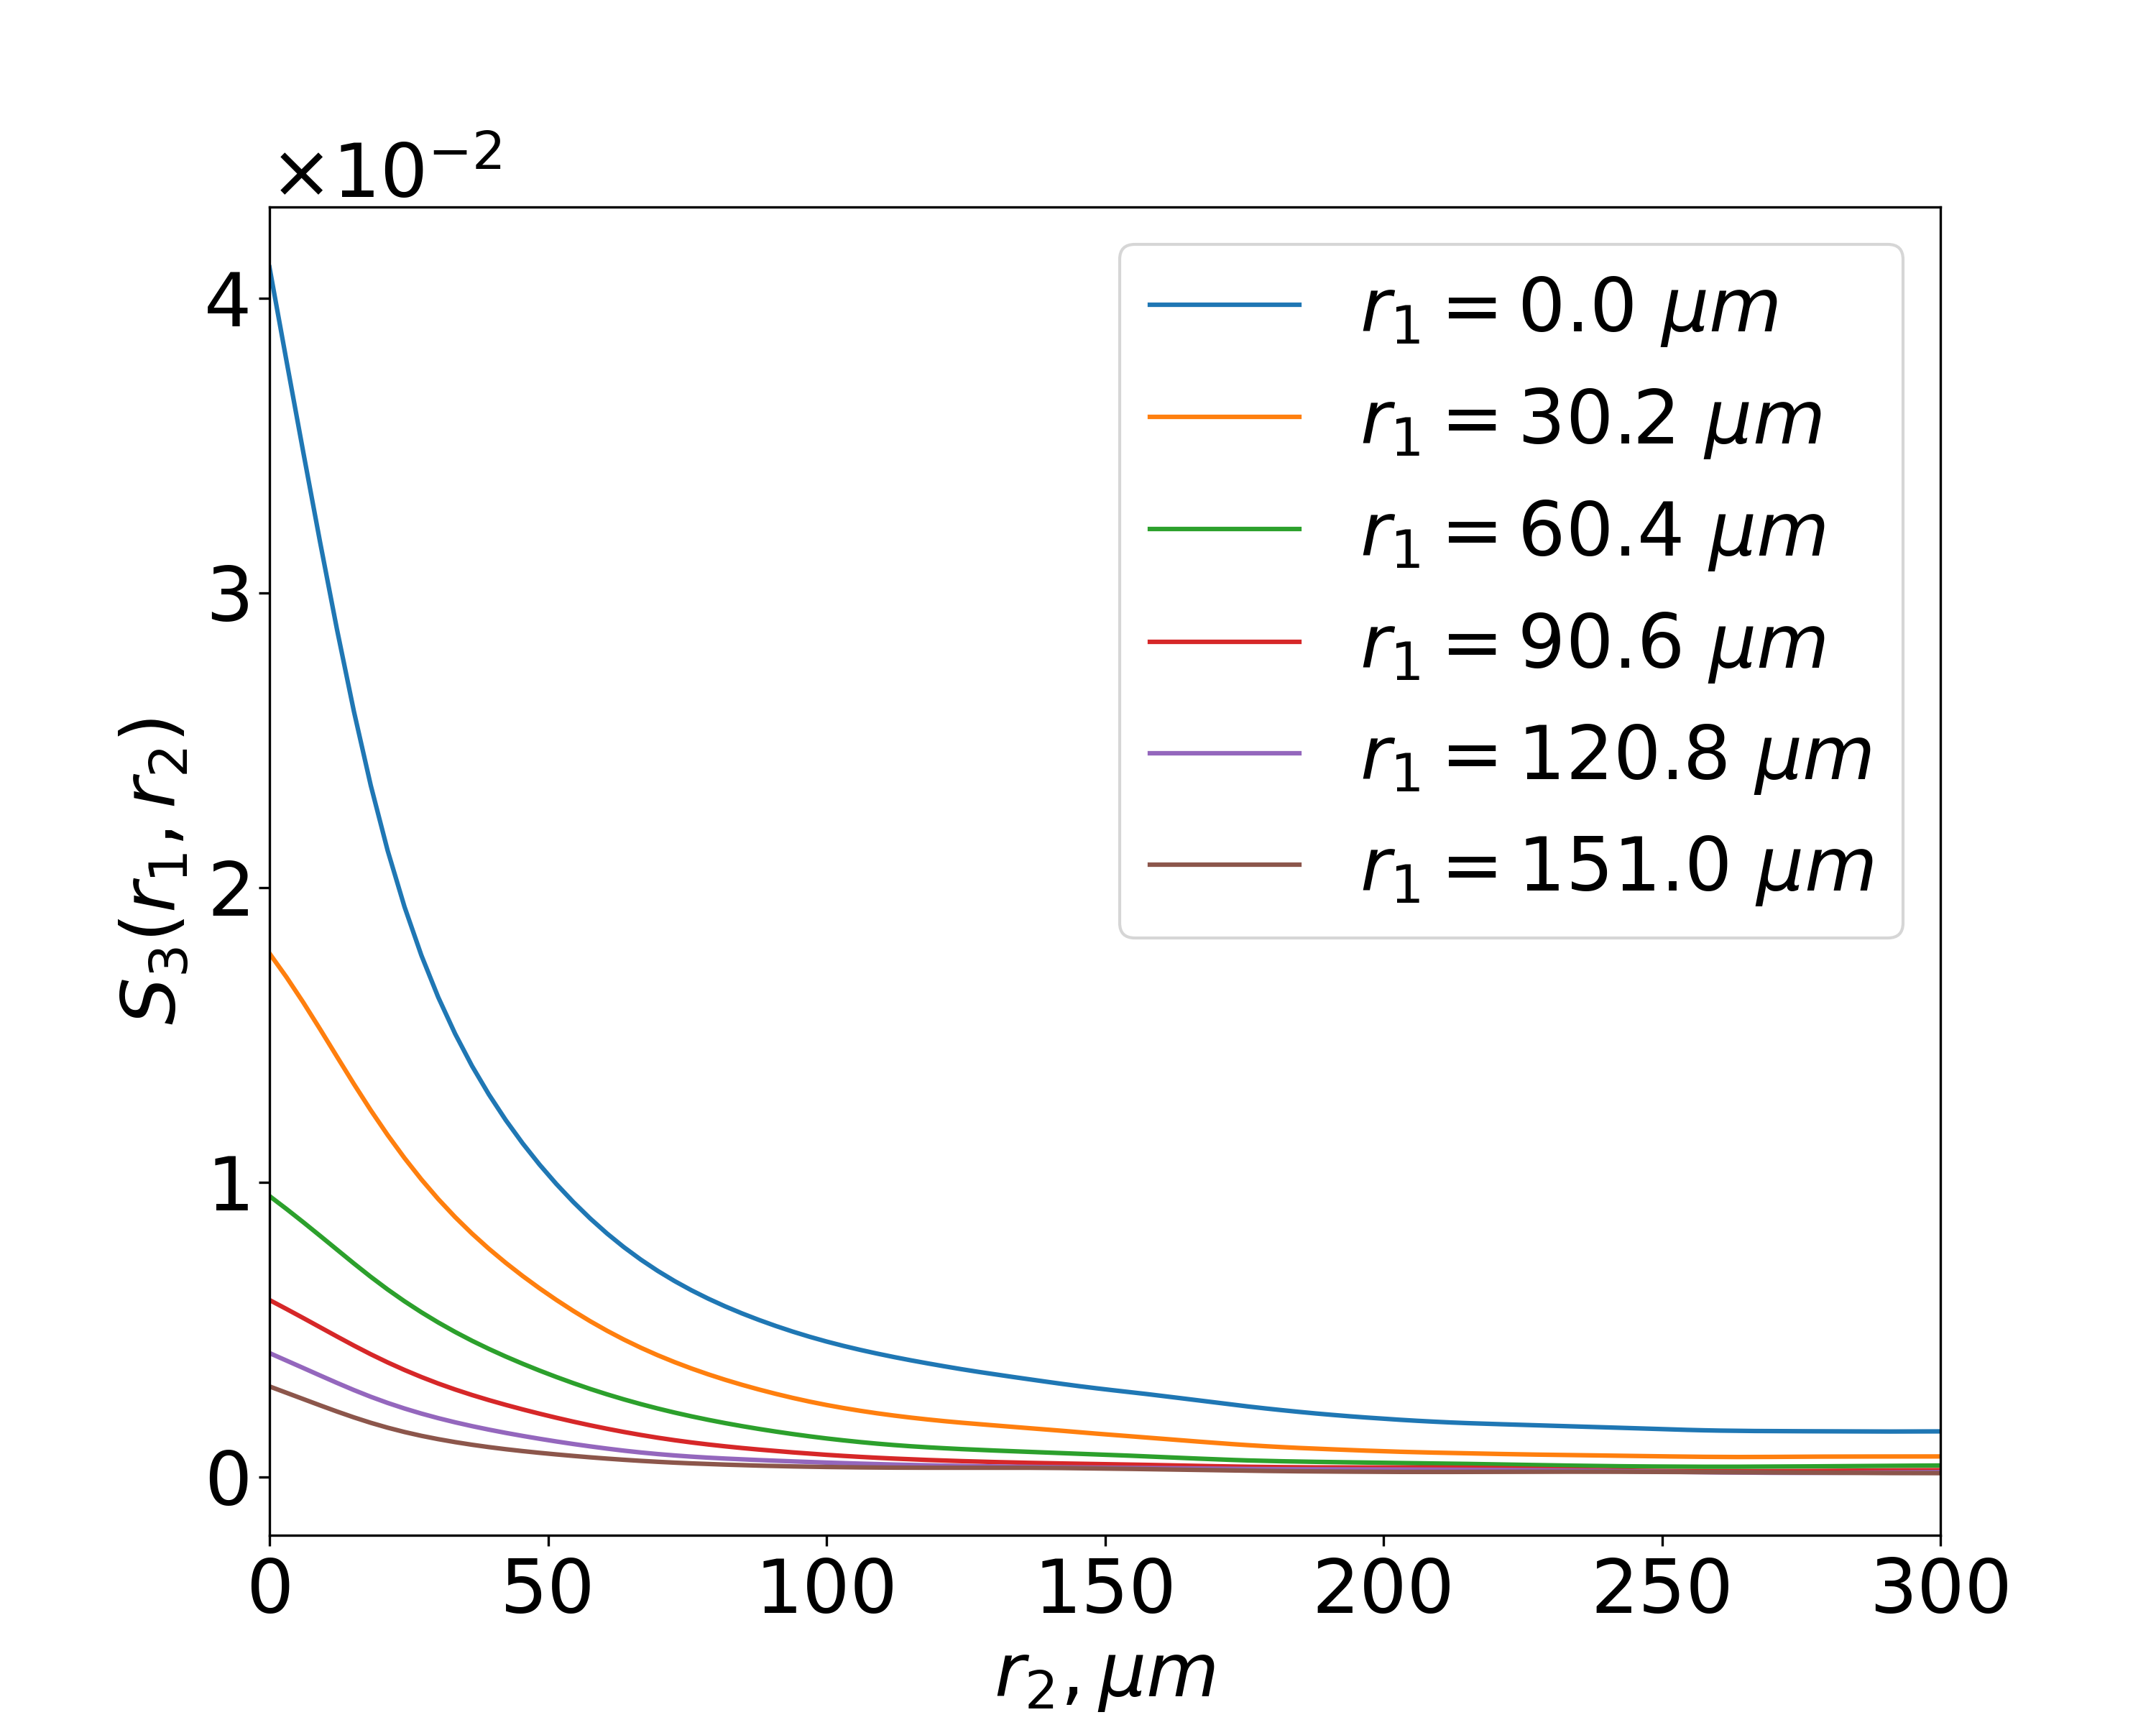
\includegraphics[width=0.45\linewidth]{images/carb.npy-s3.png}
  \vskip\baselineskip
  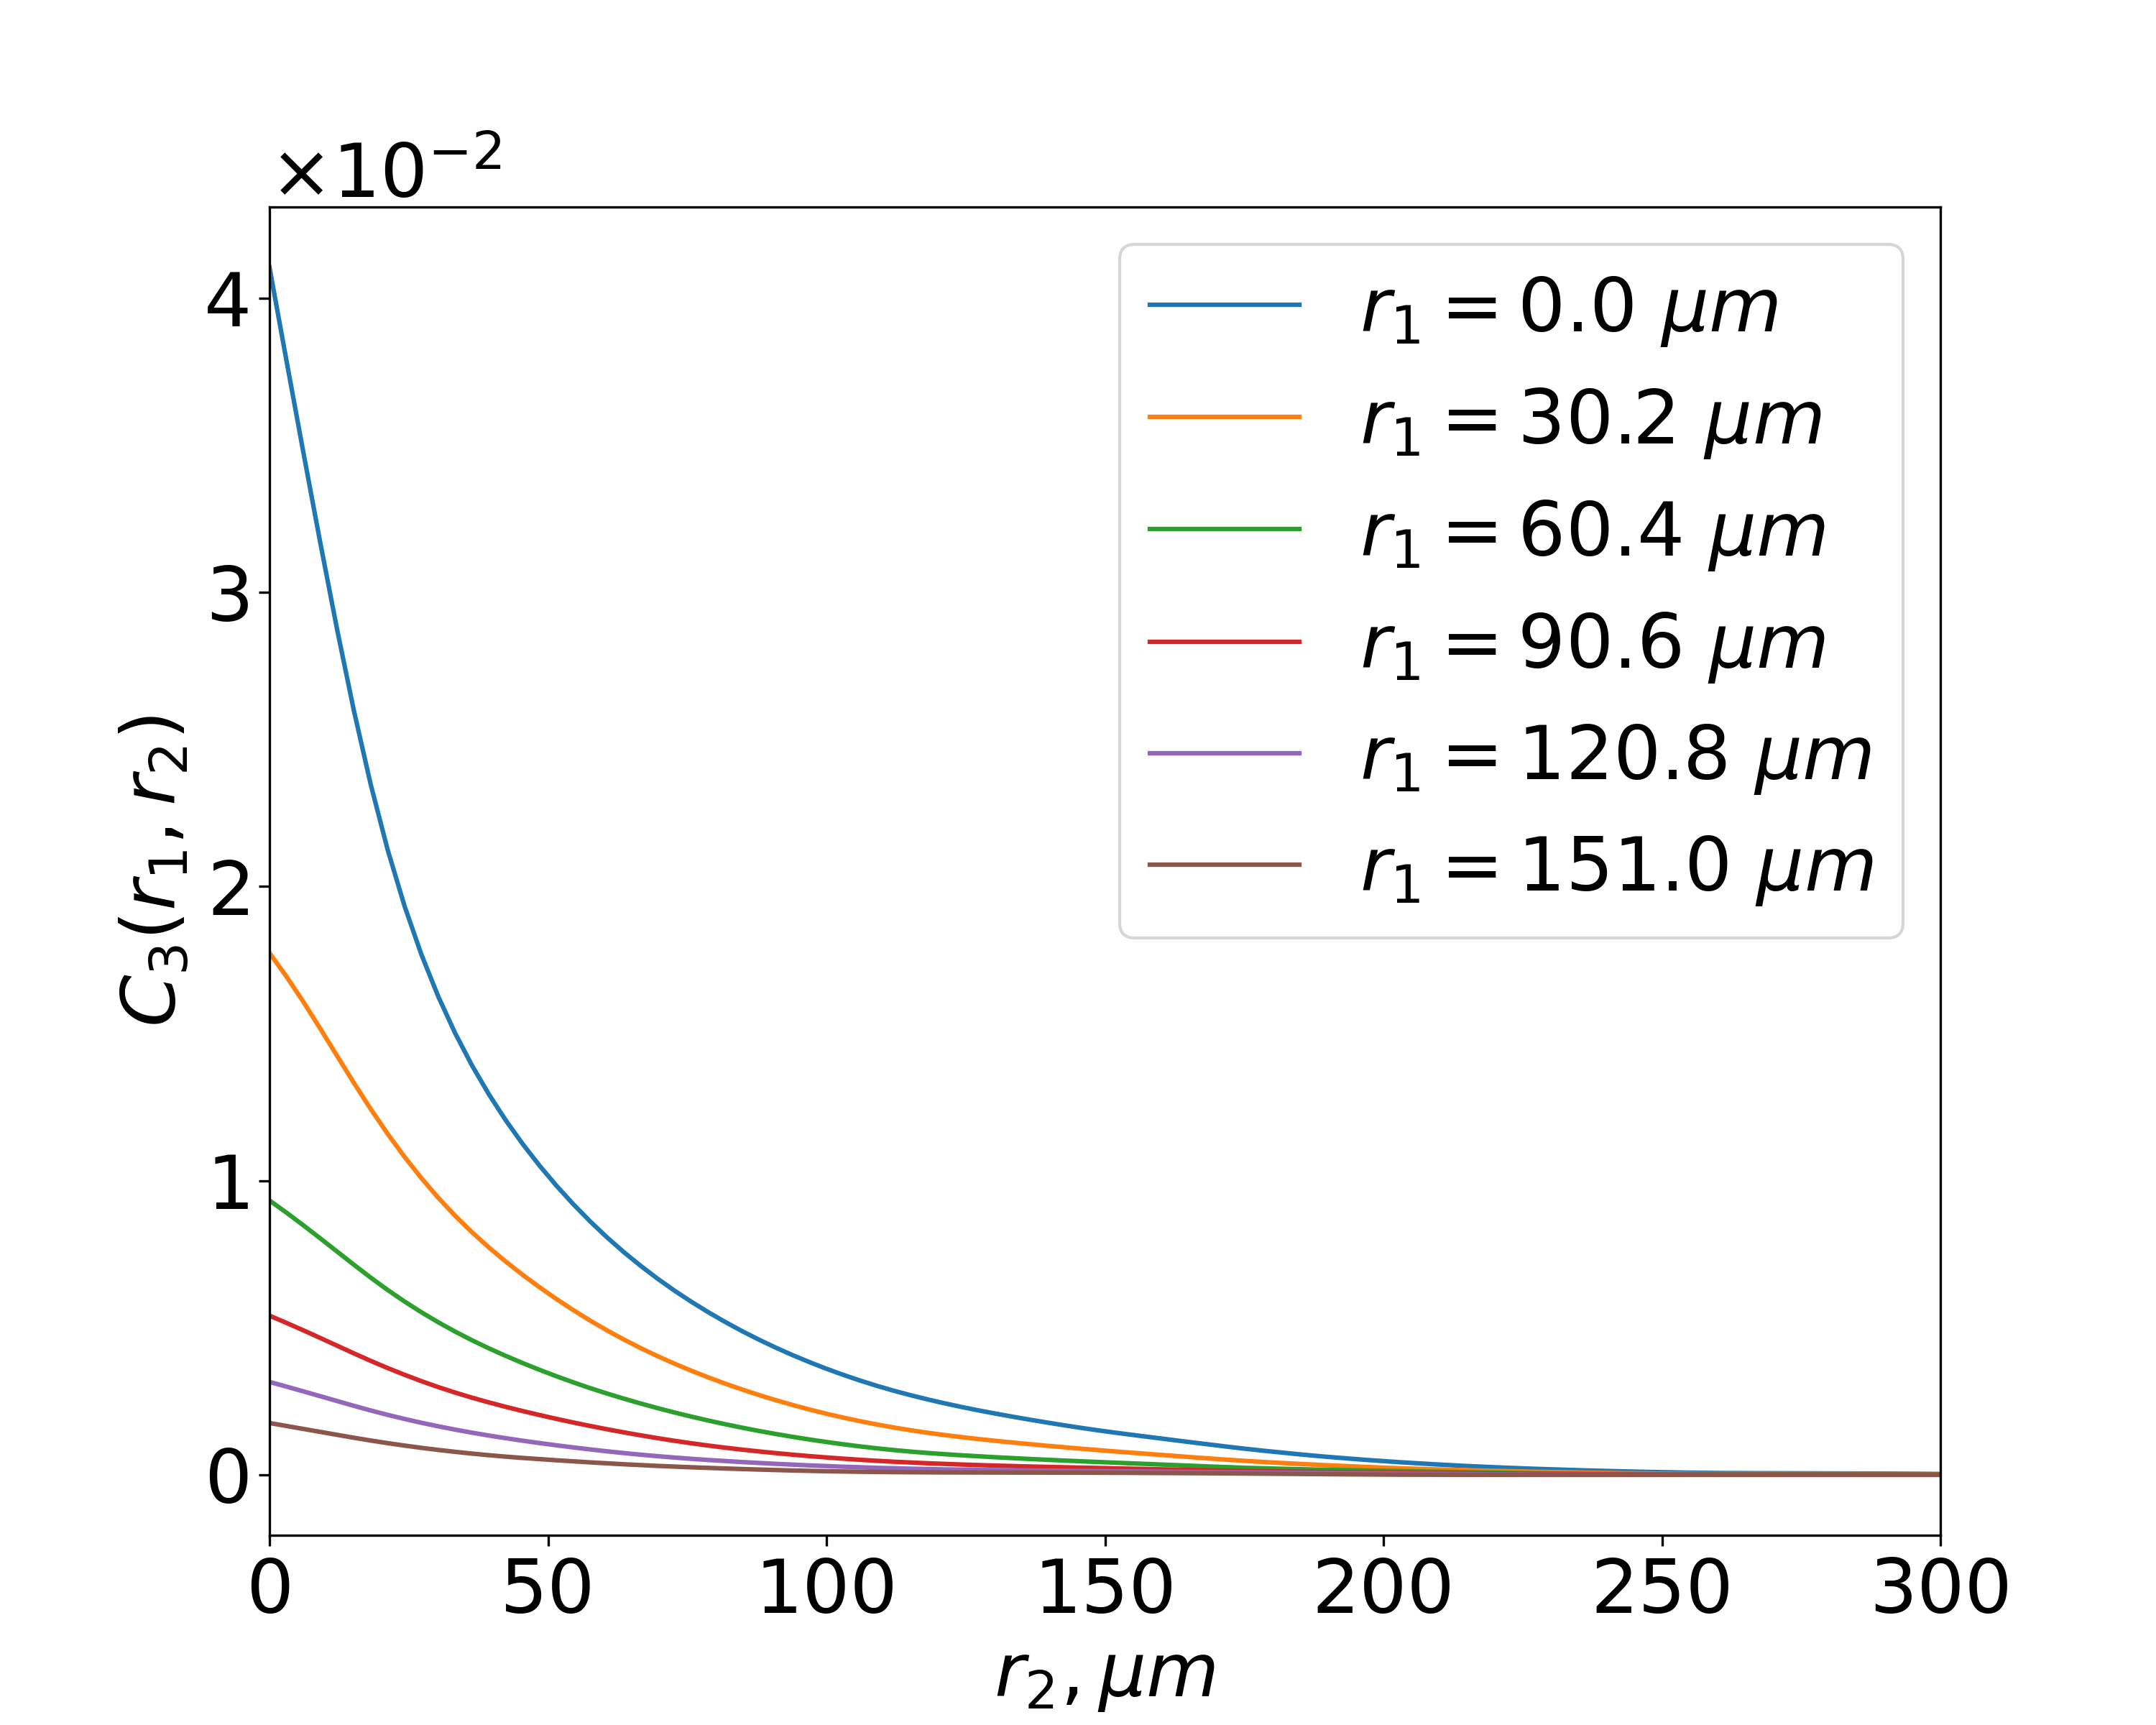
\includegraphics[width=0.45\linewidth]{images/carb.npy-c3.png}
  \caption[]{Correlation functions for carbonate sample
    (\cref{fig:sample-limestone}).}
  \label{fig:sample-limestone-cf}
\end{figure}

\begin{figure}[tp]
  \centering
  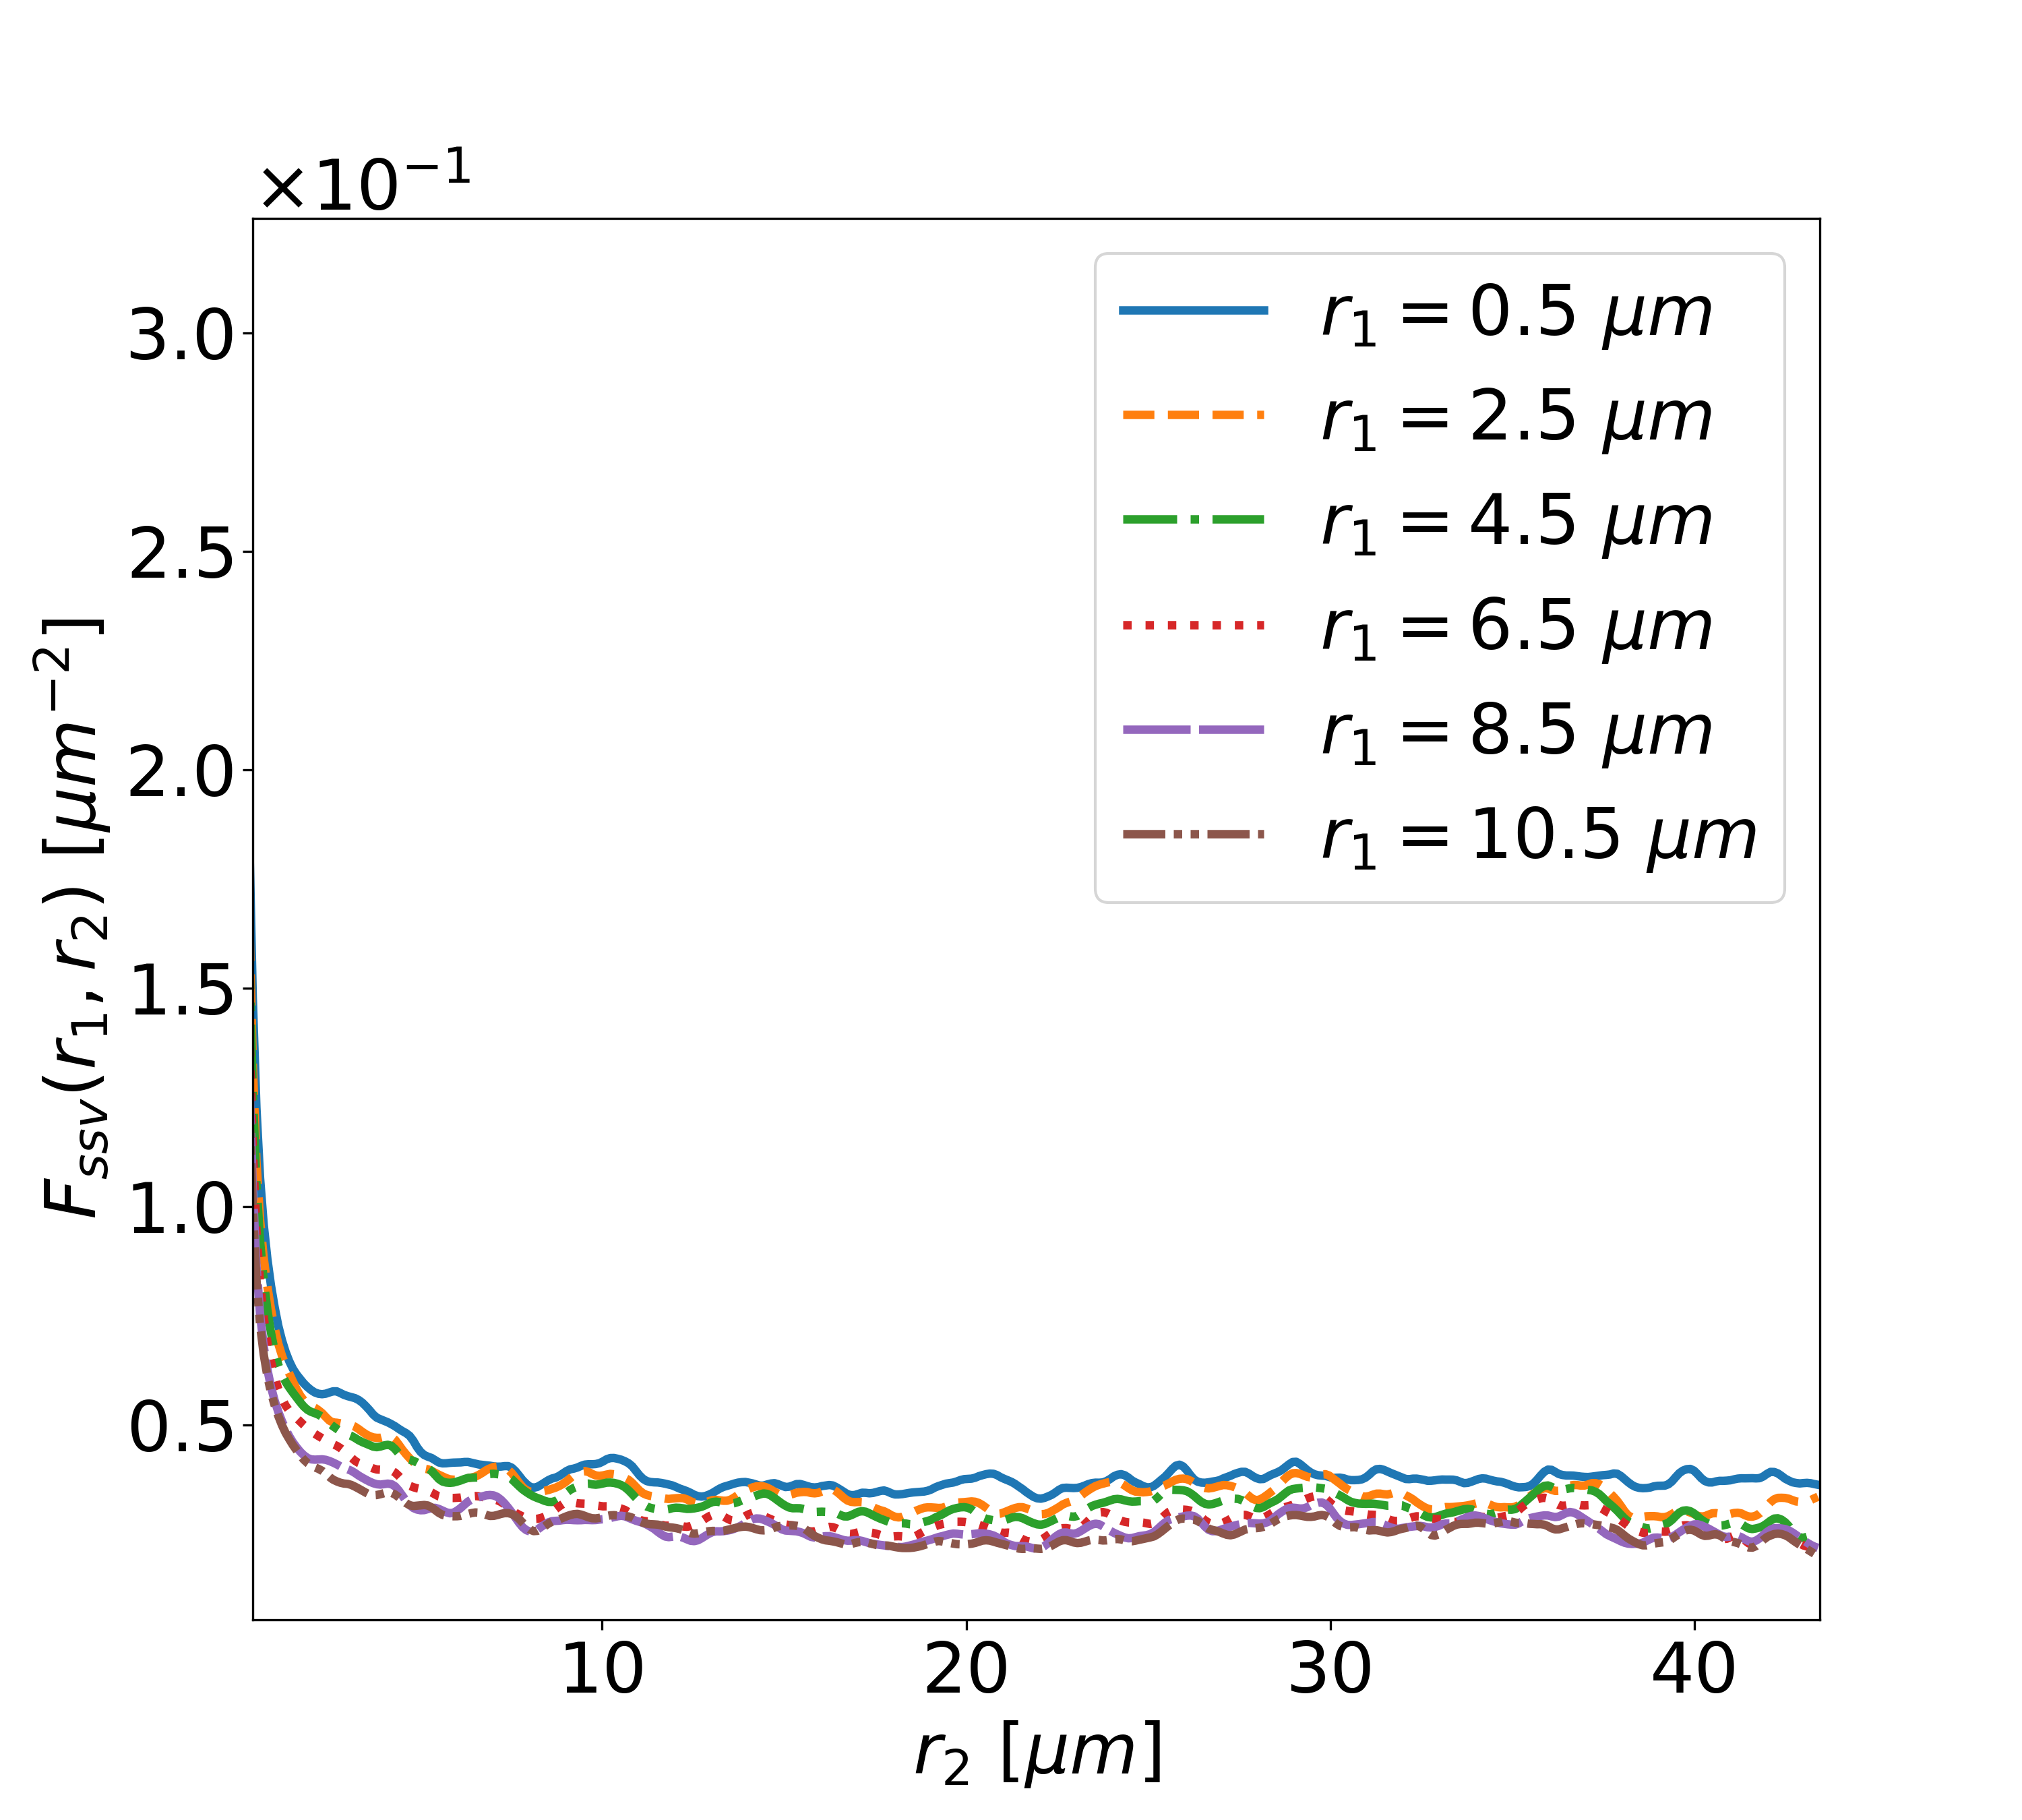
\includegraphics[width=0.45\linewidth]{images/sandstone1.png-surf2void.png}
  \hfill
  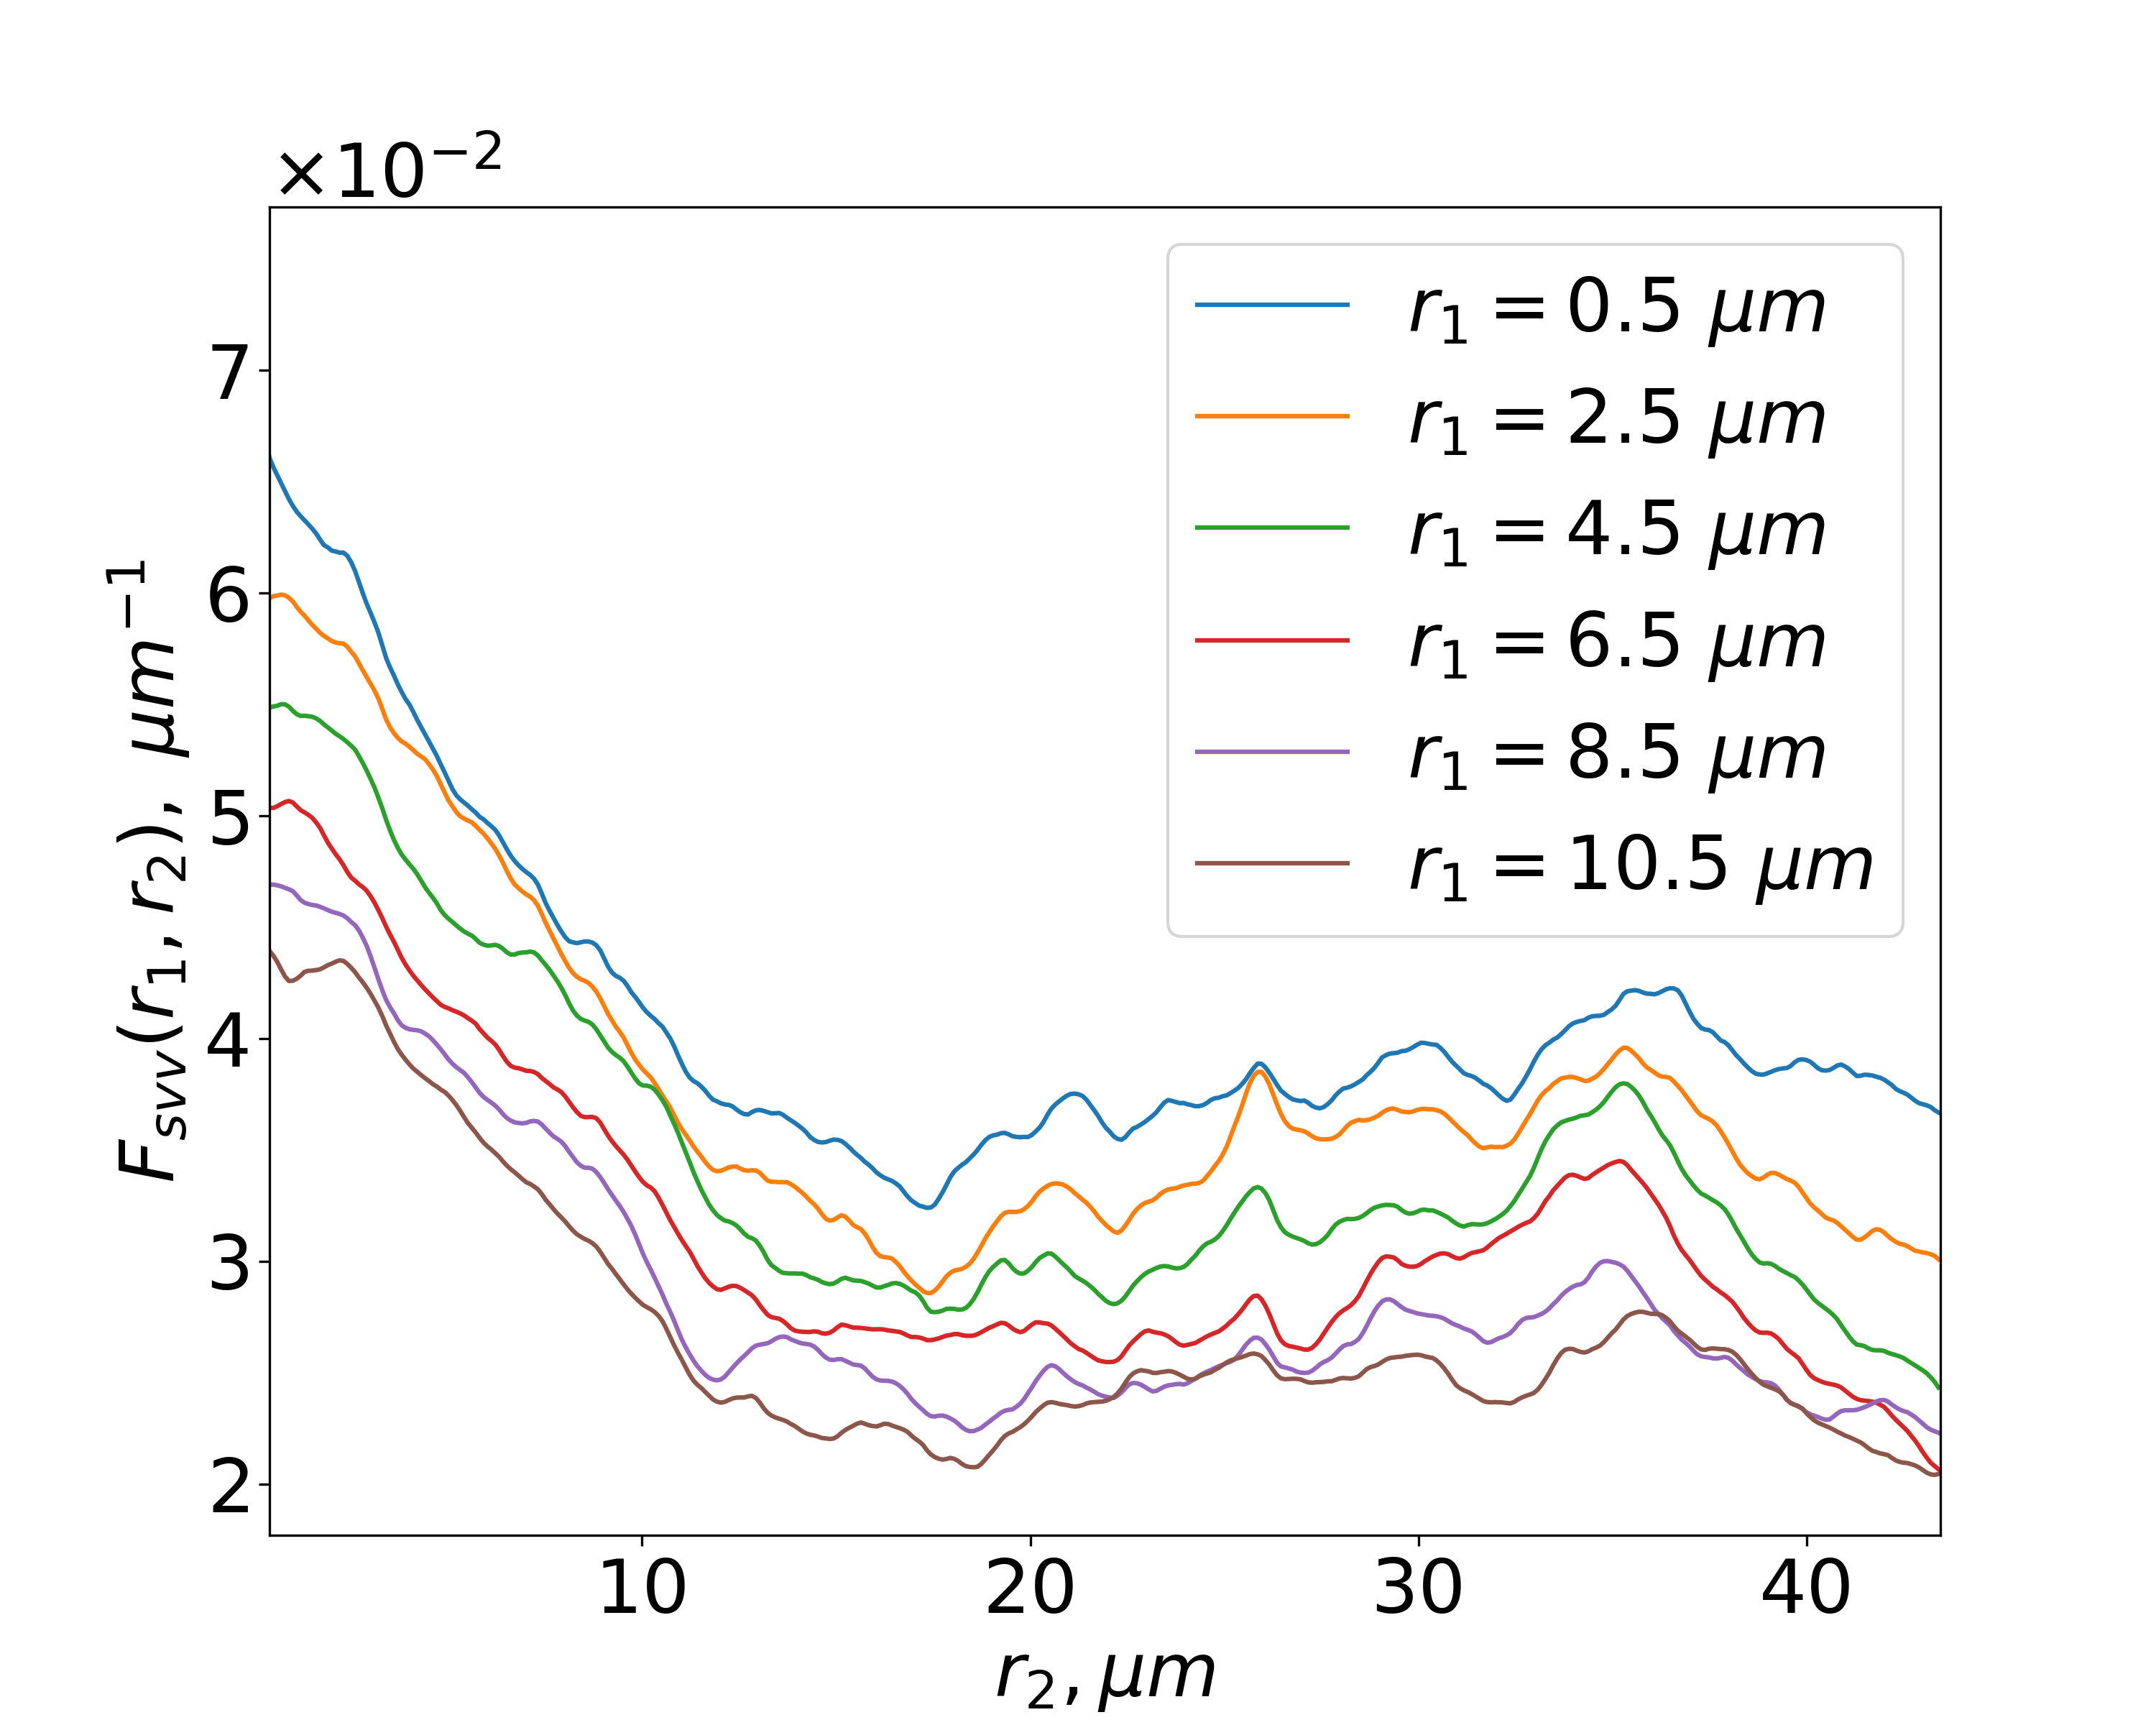
\includegraphics[width=0.45\linewidth]{images/sandstone1.png-surfvoid2.png}
  \vskip\baselineskip
  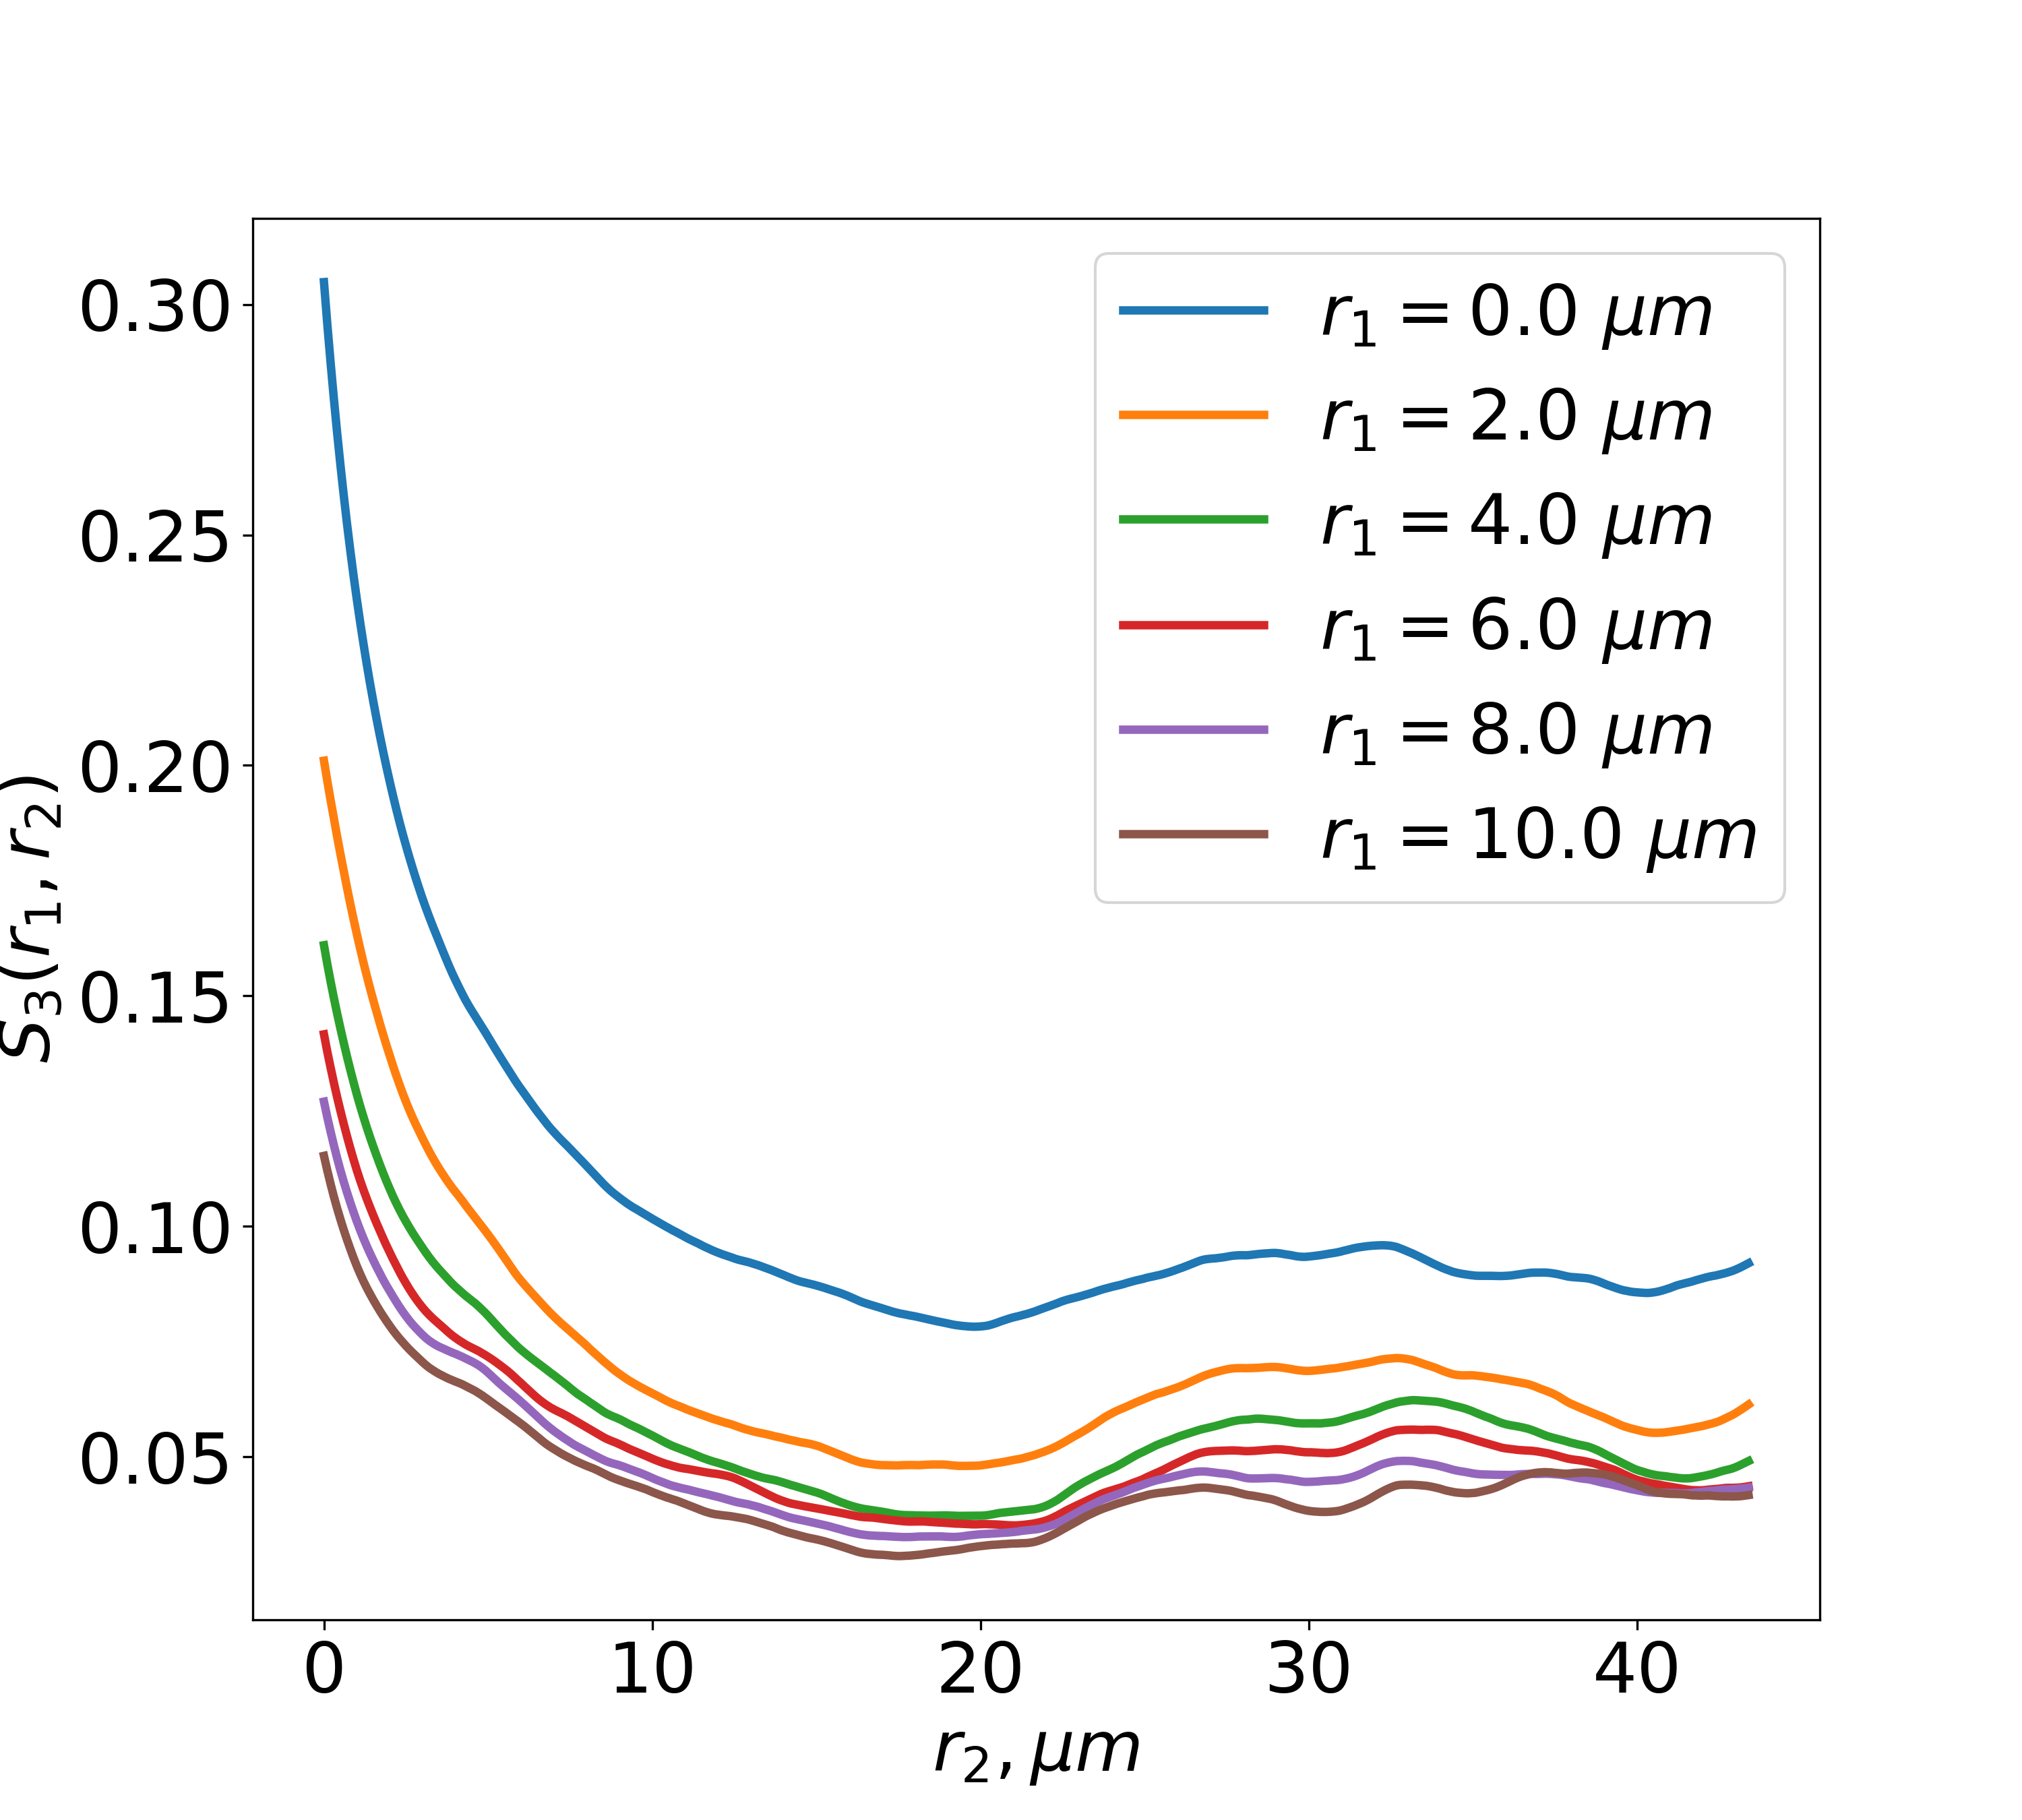
\includegraphics[width=0.45\linewidth]{images/sandstone1.png-s3.png}
  \hfill
  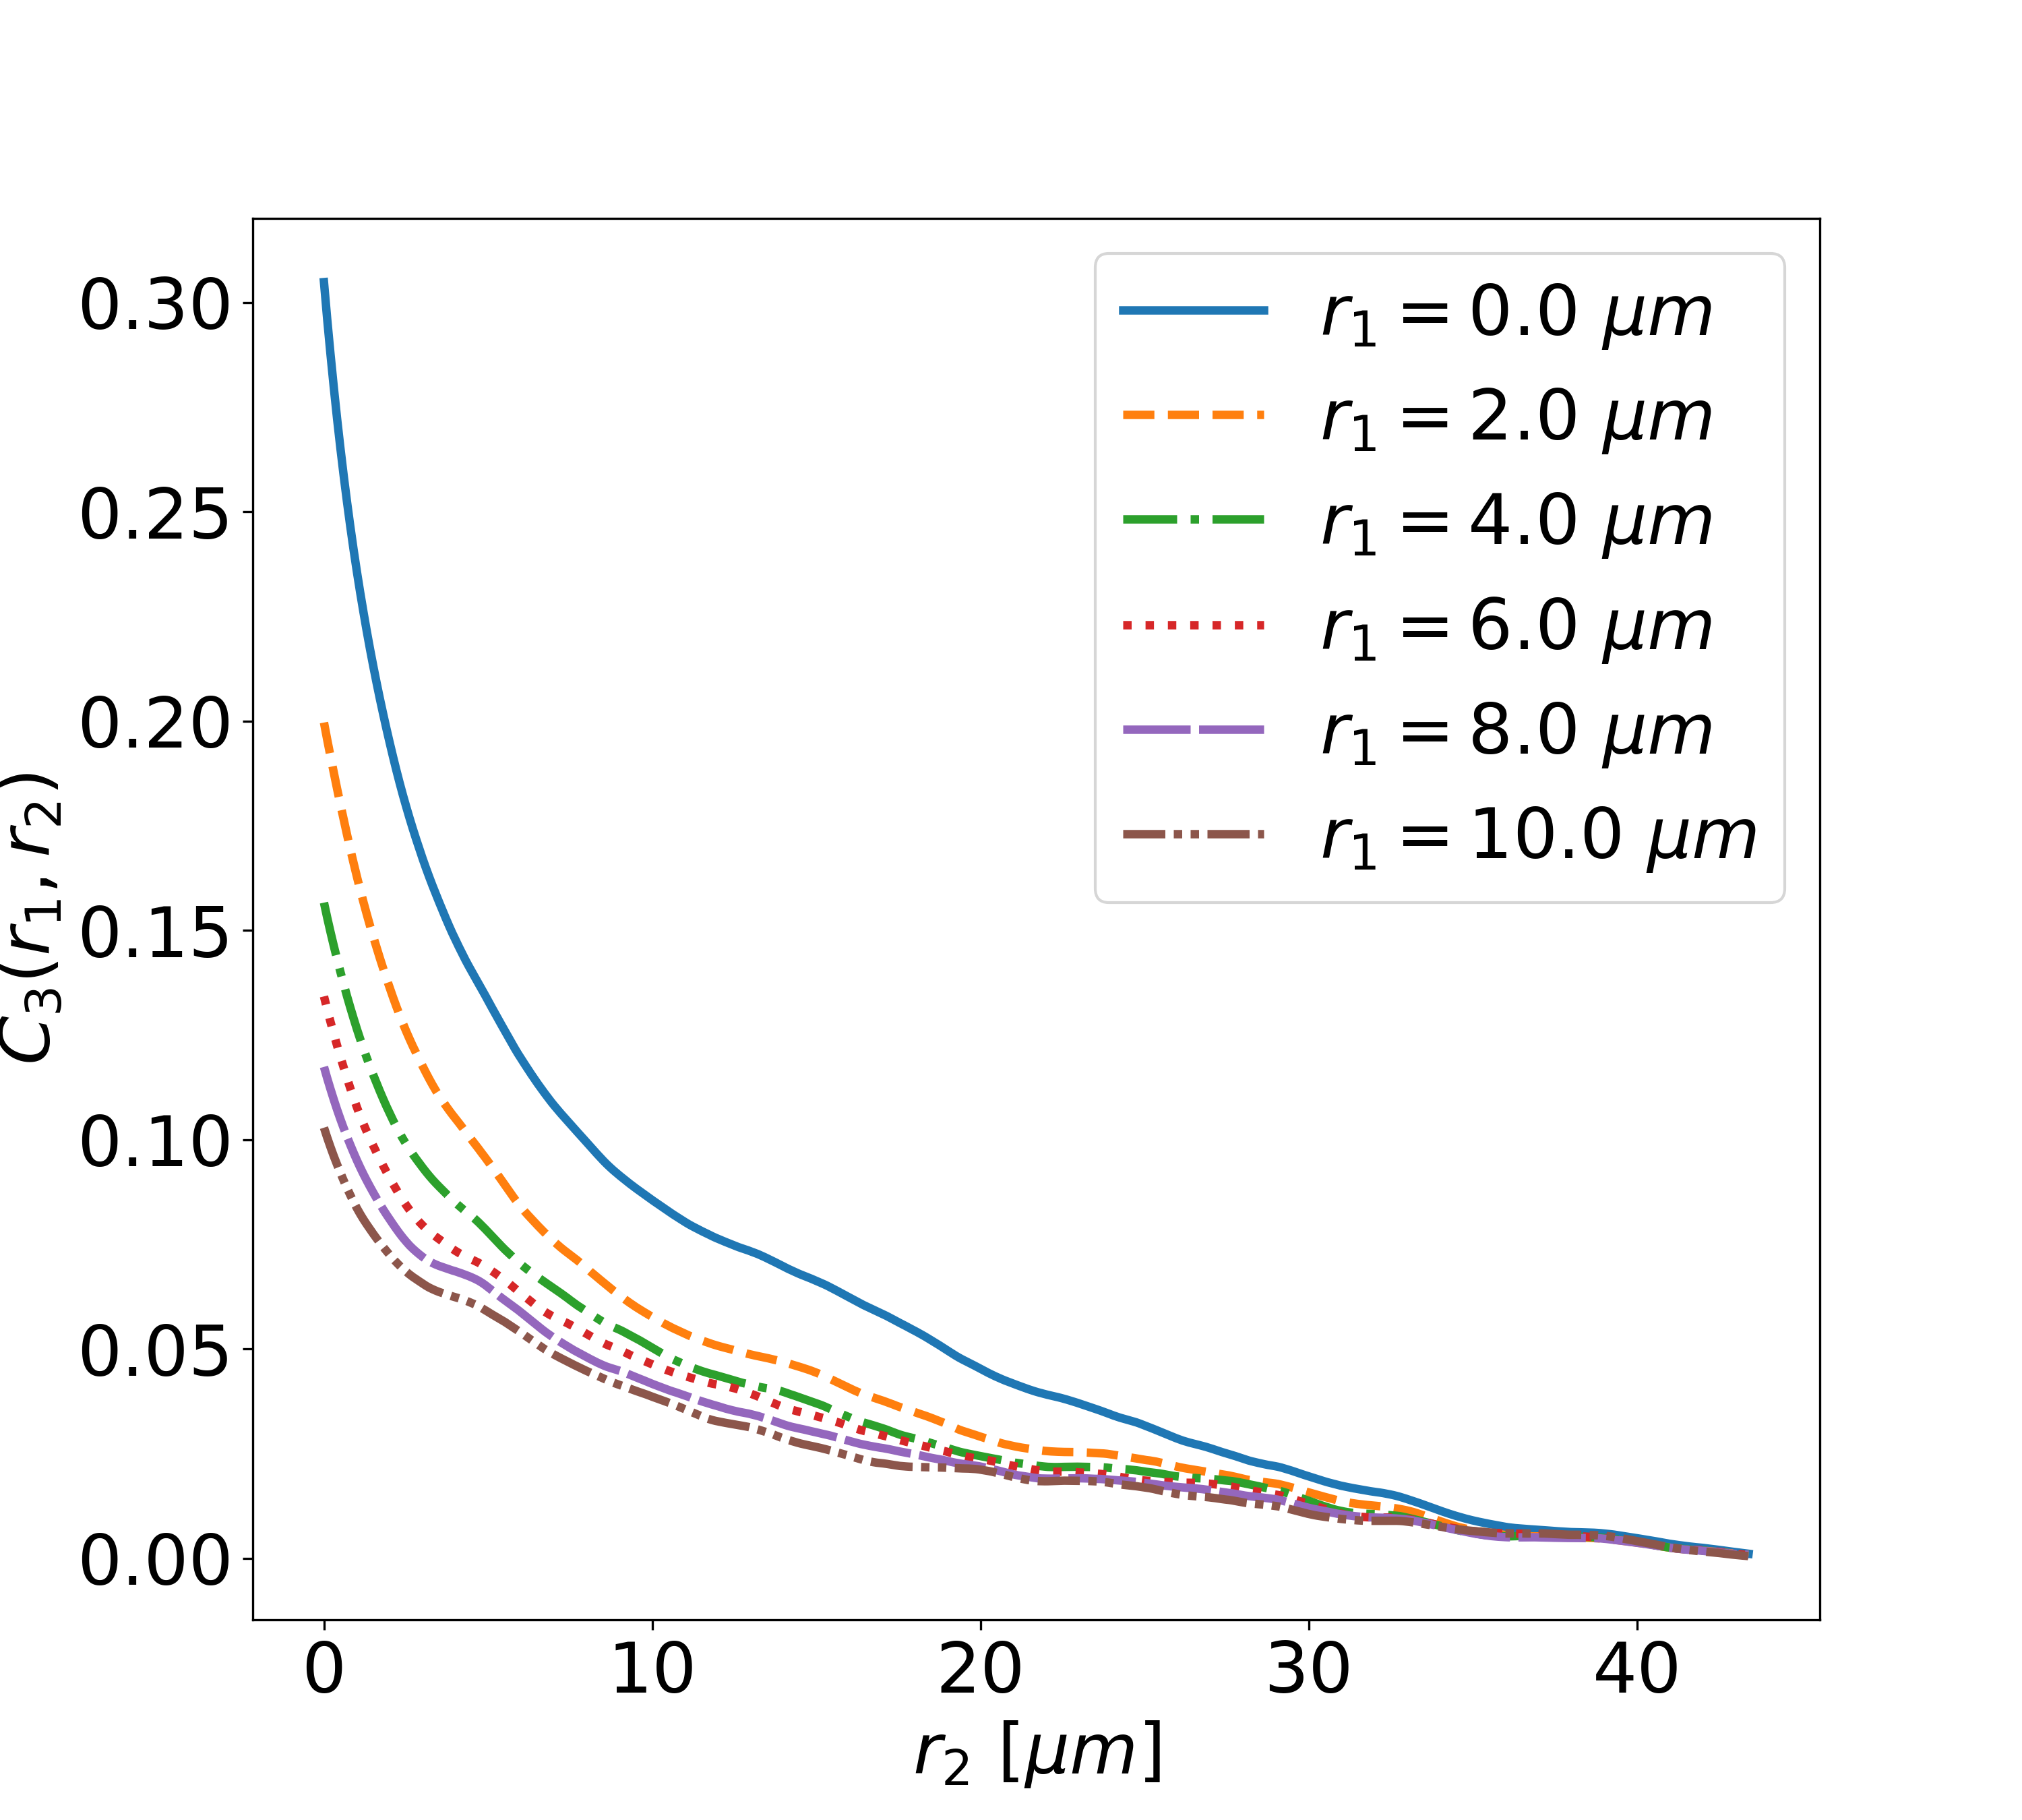
\includegraphics[width=0.45\linewidth]{images/sandstone1.png-c3.png}
  \caption[]{Correlation functions for sandstone sample
    (\cref{fig:sample-sandstone}).}
  \label{fig:sample-sandstone-cf}
\end{figure}

\begin{figure*}[tp]
  \centering
  \subfigure[Shale]{
    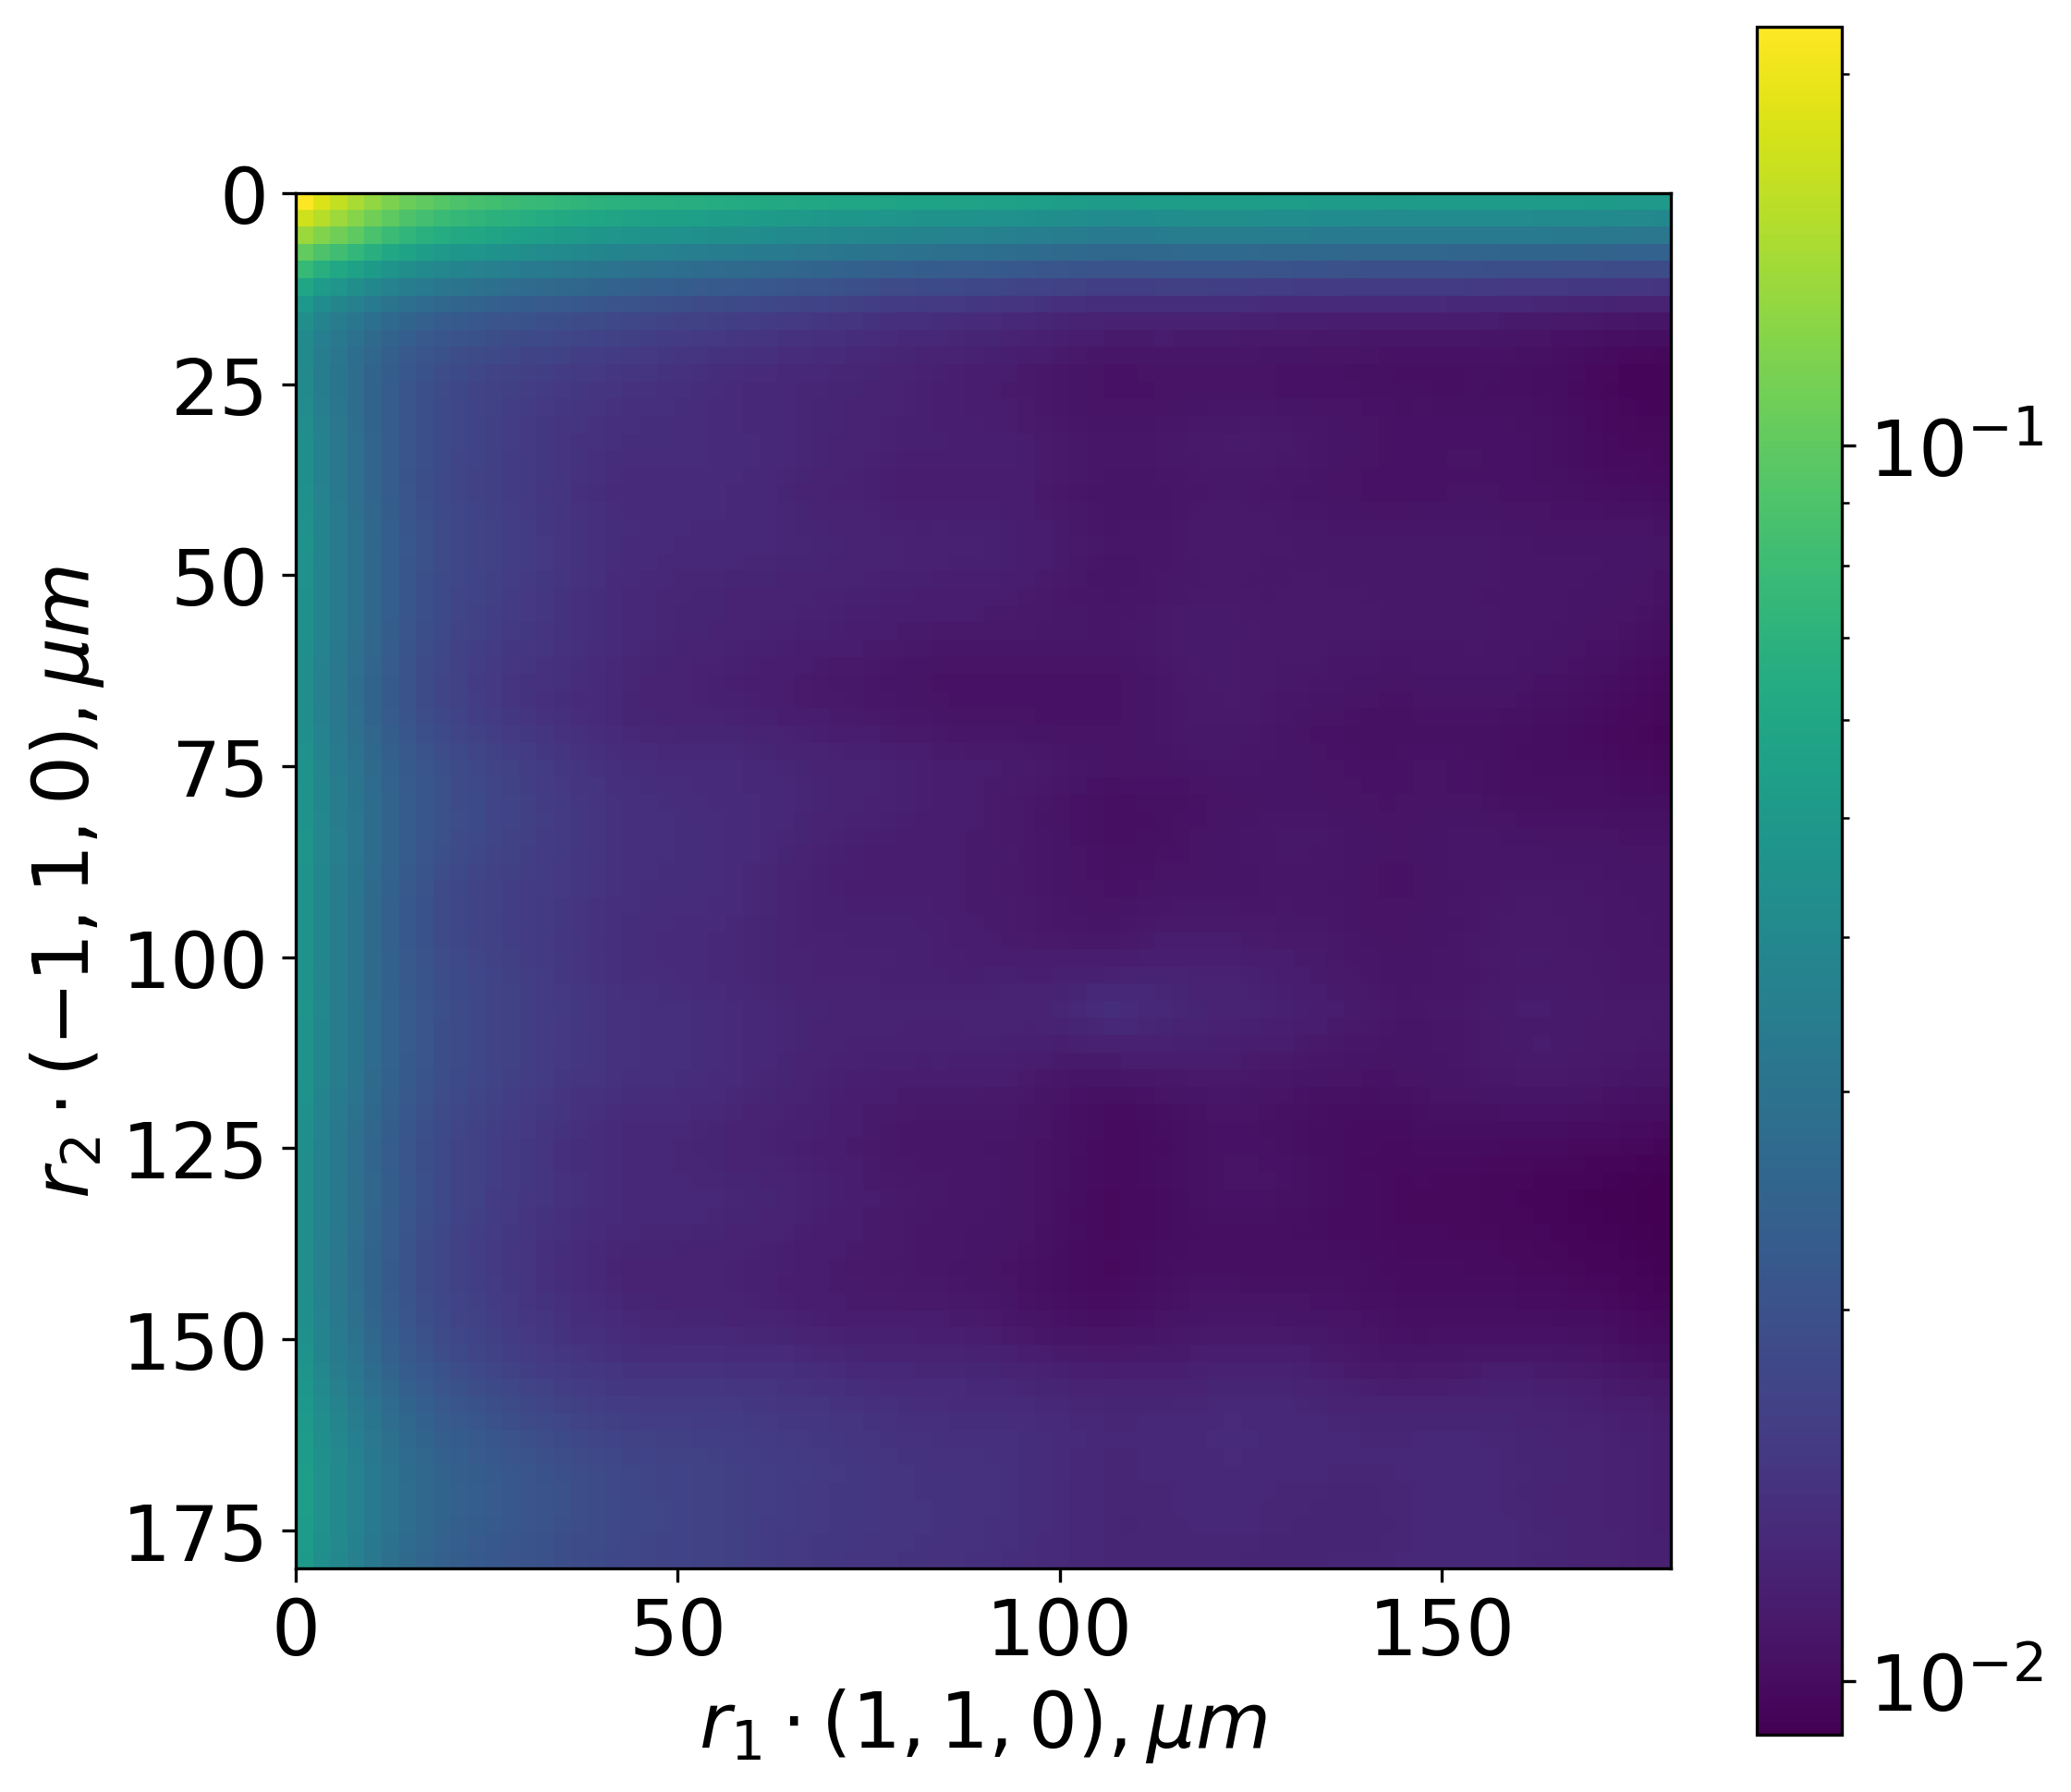
\includegraphics[width=0.45\linewidth]{images/shale-s3.png}
    \label{fig:shale-s3}}
  \hfill
  \subfigure[Soil]{
    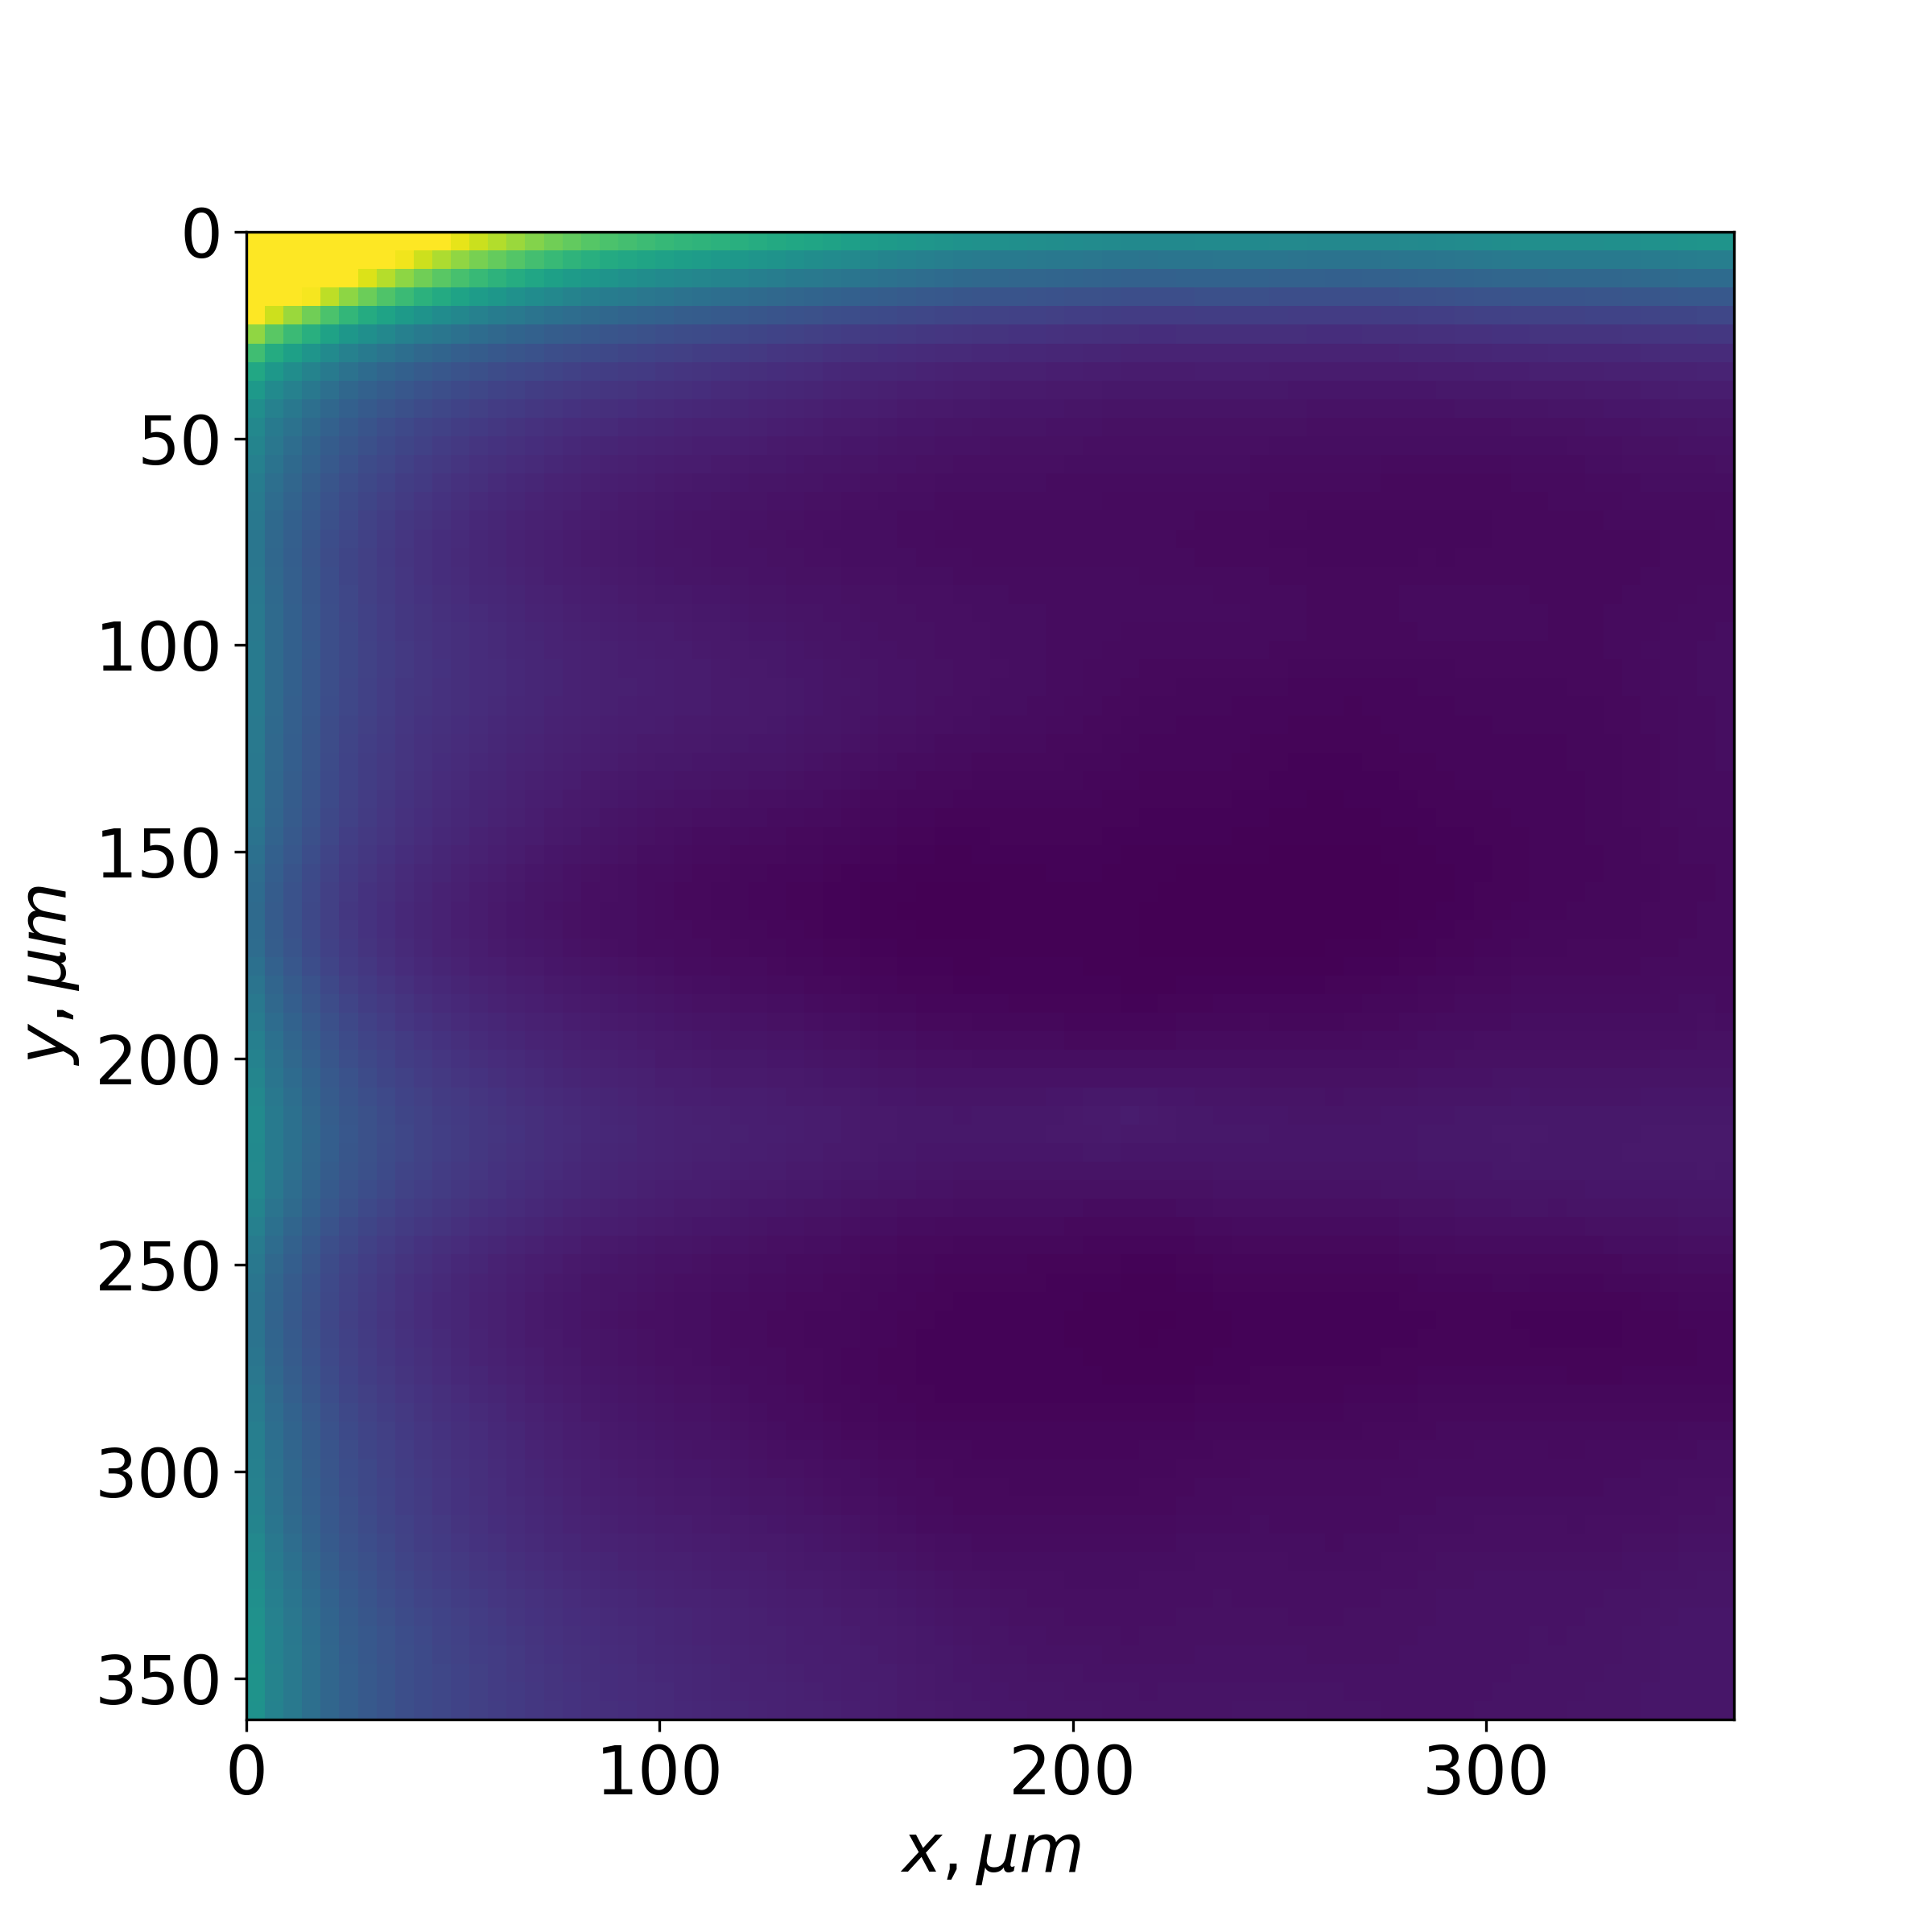
\includegraphics[width=0.45\linewidth]{images/soil-s3.png}
    \label{fig:soil-s3}}
  \hfill
  \caption[]{Heatmaps of $S_3$ function for highly anisotropic samples of shale
    and soil. $S_3$ function was clamped to the range $[0, 0.1]$ to make
    anisotropicity more visible. It can be observed that the samples have
    cavities elongated along the vector $(1, 1, 0)$.}
  \label{fig:heatmaps}
\end{figure*}

\section{Discussion}
In this paper we have provided two approaches to compute three-point correlation
function:
\begin{enumerate}
\item Computation in frequency domain using Fourier transform. This approach has
  computational complexity $O(n^2 \log n)$ and computes the whole correlation
  map. Unfortunately, it requires $O(n^2)$ additional memory and therefore can
  be used only with small inputs. Moreover, the whole Fourier image of the input
  is needed even if we need only a small part of the correlation map.
\item Computation in spatial domain. This approach is implemented by us in
  CorrelationFunctions.jl package. This approach calculates the full map with
  complexity $O(n^3)$ but uses only $O(n)$ additional memory for shifted
  versions of the input. For our purposes the whole map is not needed and
  therefore the amount of calculations can be significantly reduced.
\end{enumerate}
It's tempting to create an algorithm which unites advantages of both approaches
(fast speed of the first and low memory consumption of the second) which
computes some desired slices of correlation map. It is known that Fourier
transform is the only linear transform which allows computation of convolution
in linear time. It is still an open question if there are linear transforms which
allow computation of convolution faster than a naïve approach
\cite{stone2008uniqueness,stone1998convolution}.

\textcolor{red}{Where to put this?}
We have made a comparison of our algorithm with two algorithms, one of which
proposed by Malmir~et~al \cite{malmir2018} and another proposed by Smith and
Torquato \cite{SMITH1988176}. The first algorithms generates a triangle with
fixed sides $r_1$ and $r_2$ and an angle $\theta$ between them and places it in
the medium firstly making a random translation and a rotation around a random
vector by a random angle. By making a large number of trials the algorithm gets
a value of a three-point correlation function at the point
$(r_1, r_2, \theta)$. The second algorithm takes a precalculated triangle
$(r_1, r_2, \theta)$ from a web-like pattern and places it in the medium without
rotation, only applying a random translation. This way the algorithm preserves
orientation of triangles stored in the pattern.

Our algorithm fixes $\theta = \frac{pi}{2}$ and does not perform random
rotations or trial triangles. It is sensitive to anisotropicity of the medium
when it is stretched along one of the axes as shown in \cref{fig:aniso}. The
main advantage of our algorithm is its parallelizability and ease of
implementation. An equivalent operation for rotation of test triangles is a
rotation of the whole input image which we have implemented in our
CorrelationFunctions.jl package. By applying a rotation to the input first we
made a rest of the algorithm cache-friendly by avoiding random memory access.
\begin{figure}[tp]
  \centering
  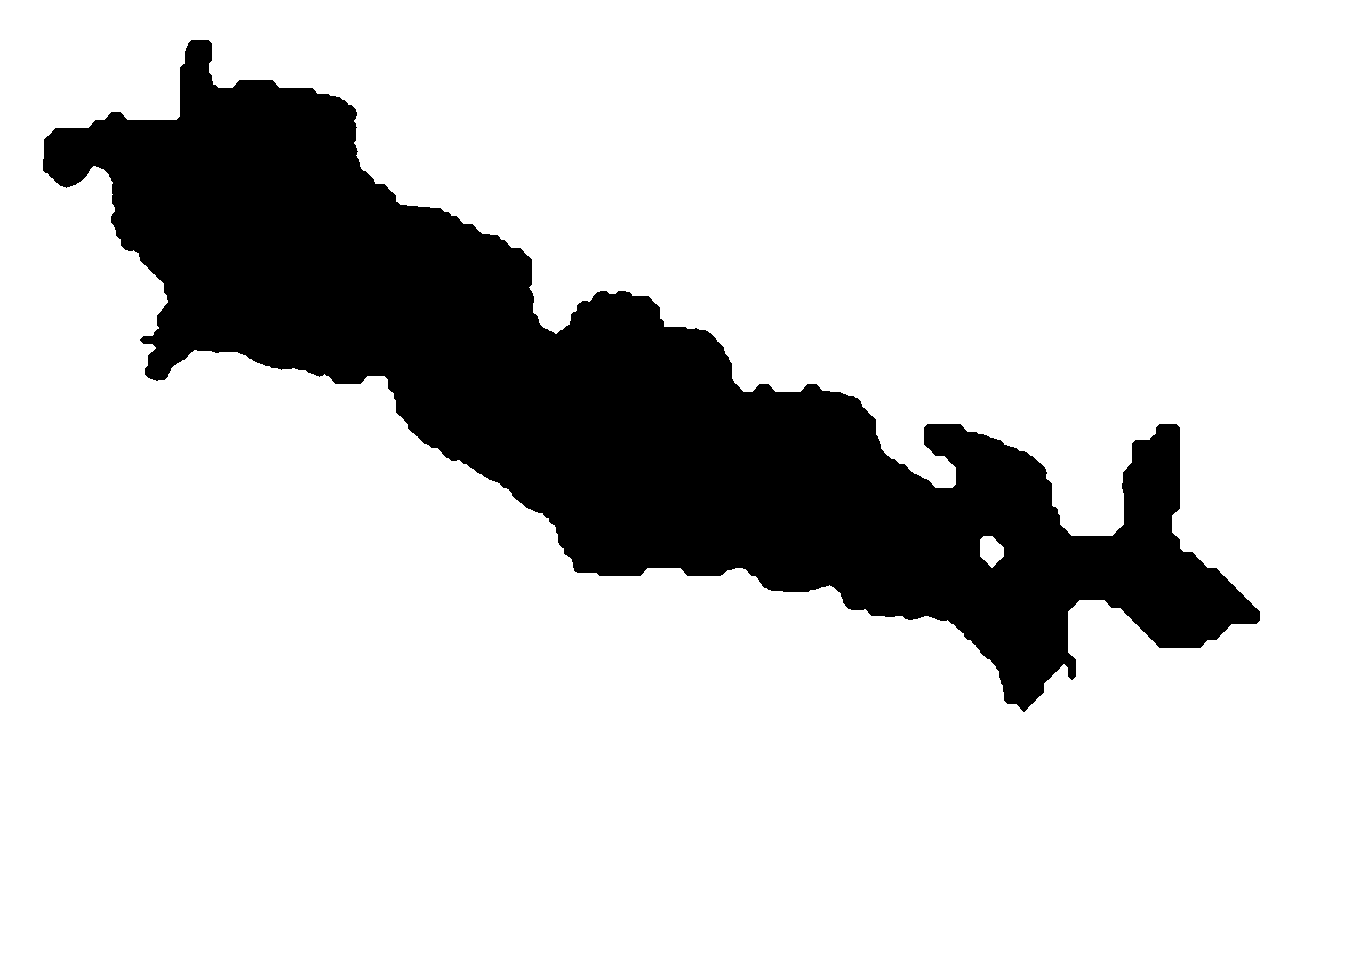
\includegraphics[width=0.4\linewidth, frame]{images/aniso.png}
  \vskip\baselineskip
  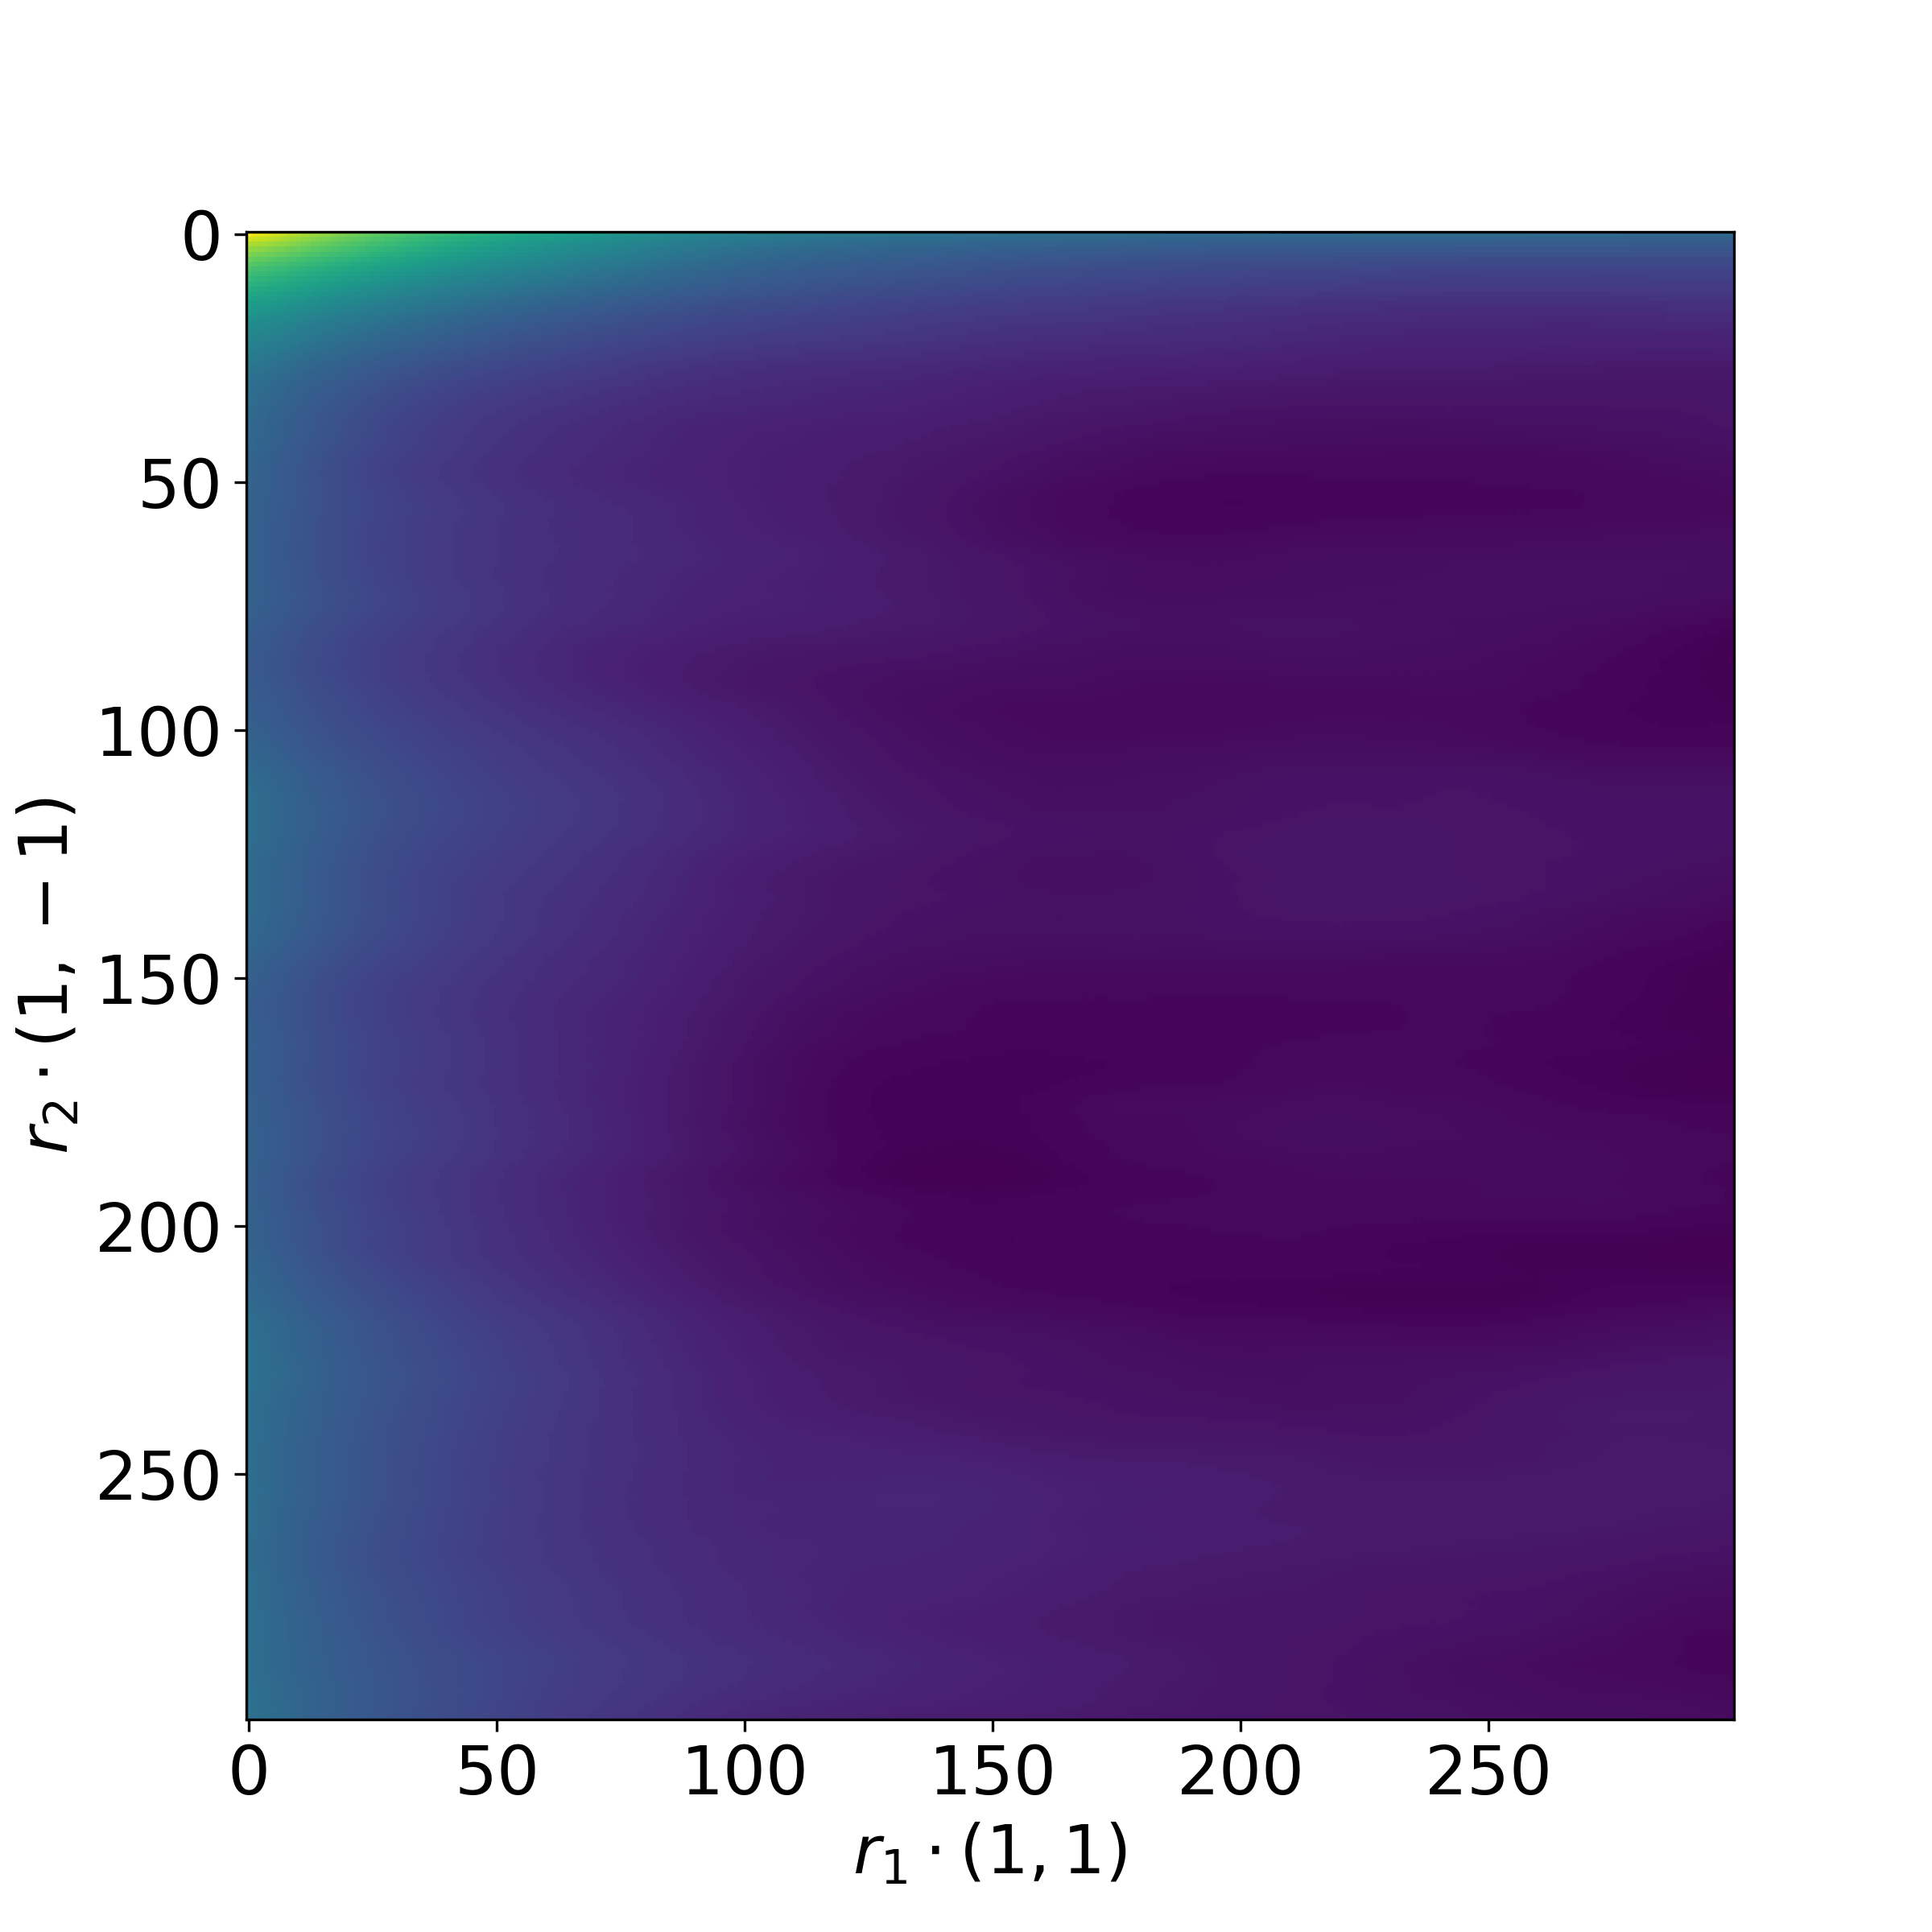
\includegraphics[width=0.45\linewidth]{images/aniso-s3.png}
  \hfill
  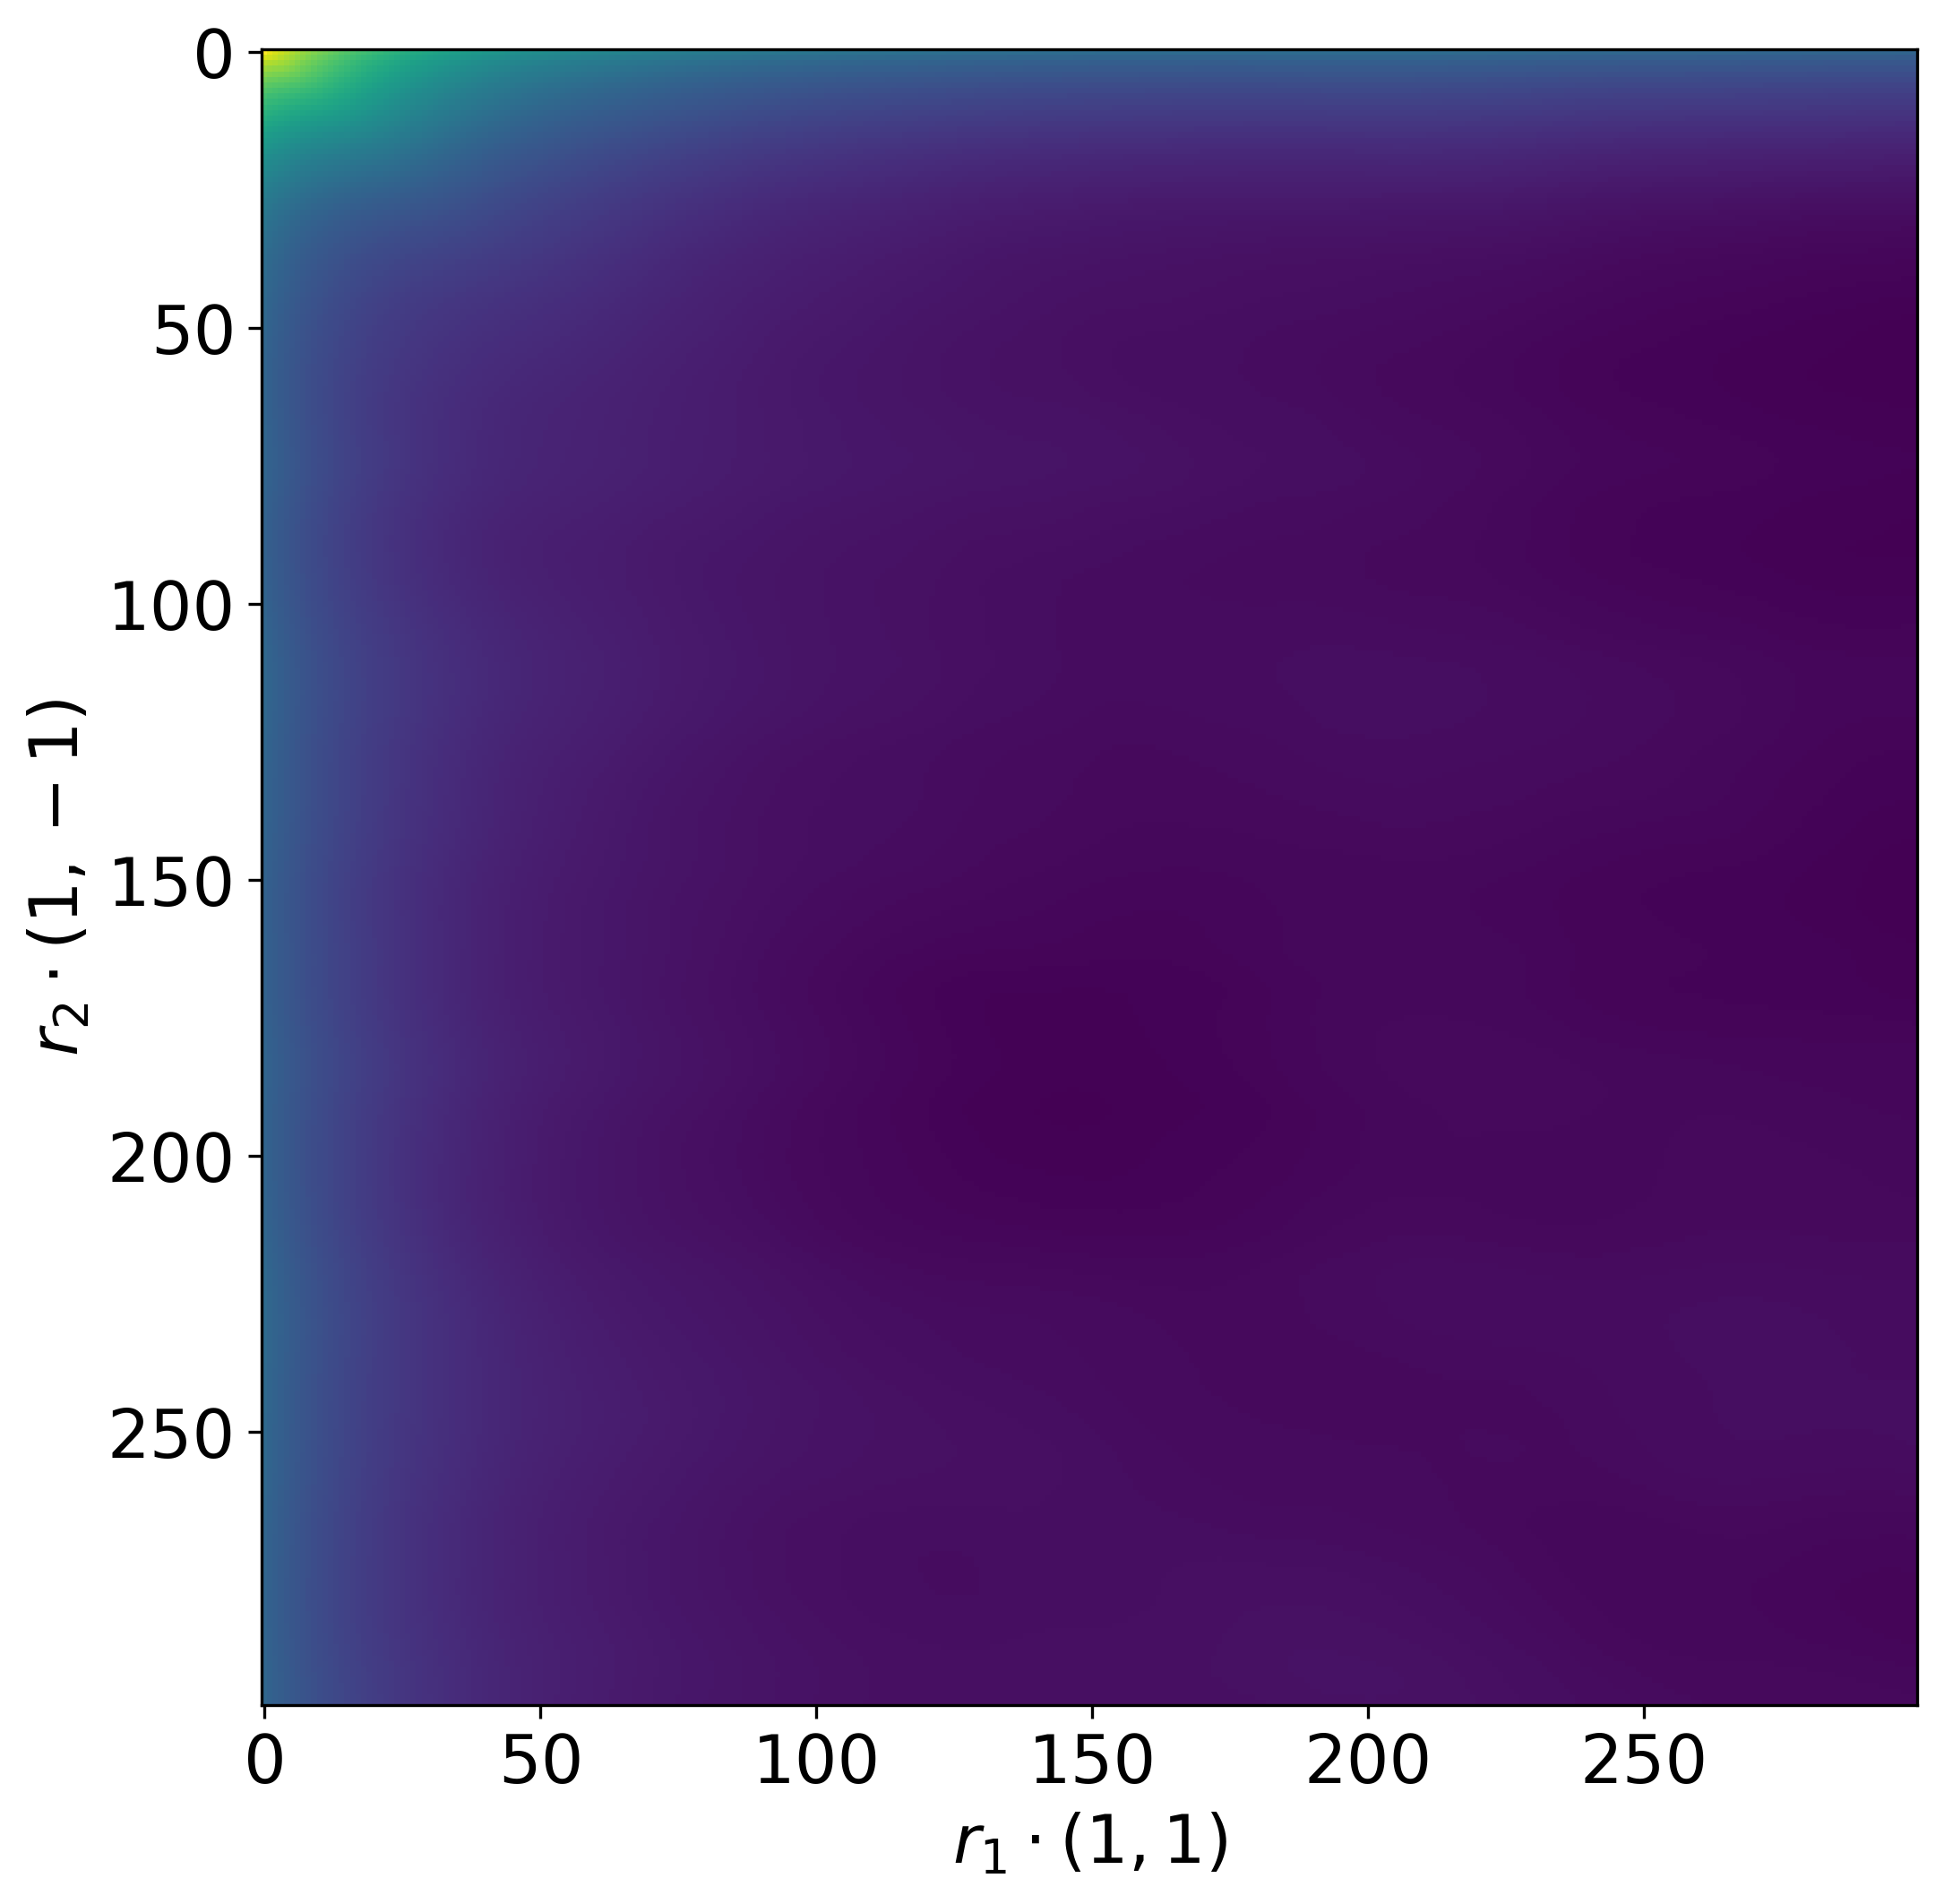
\includegraphics[width=0.45\linewidth]{images/aniso-s3-avg.png}
  \caption[]{$S_3$ function for anisotropic media (on the left) elongated along
    the vector $(1, 1)$. Anisotropicity of the medium can be seen on a heatmap
    of $S_3$ function (in the middle). An average of 120 $S_3$ evaluations of
    the medium rotated by a random angle is on the right.}
  \label{fig:aniso}
\end{figure}

\appendix
\section{Computation of number of trials for non-periodic mode}
\label{sec:number-of-trials}
If the displacement vectors $x_1, x_2: x_1 \perp x_2$ are parallel to two
distinct unit vectors $i=(1,0,0)$, $j=(0,1,0)$ or $k=(0,0,1)$ then the number of
trials for the input array having dimensions $D = (D_x, D_y, D_z)$ is the
following:
\begin{equation}
  \begin{aligned}
    & Norm(A, x_1, x_2) = \prod_k D'_k \\
    & D' = D - x_1 - x_2
  \end{aligned}
\end{equation}

\section{Edge detection filter}
\label{sec:filter}
For edge detection we use a kernel with the width 7 with coefficients inversely
proportional to distance to kernel's central element. The central element has
such value, so all elements of the kernel sum to zero:
\begin{equation}
  E_k = S \left\{
  \begin{array}{ll}
    -\sum\limits_{\substack{l \\ l \ne 0}} E_l & \quad k = 0 \\
    1 / \rho(k, 0) & \quad \text{otherwise}
  \end{array}
  \right.
\end{equation}
For 3D case $S=172.96$ and for 2D case $S=30.46$.

\bibliography{paper}
\end{document}
